%%!TEX encoding = UTF-8 Unicode

% According to UA rules, font size should range from 10 to 12pt.
\documentclass[11pt,a4paper,openright,twoside,onecolumn]{memoir}

\listfiles
\fixpdflayout

\usepackage[utf8]{inputenc}

% Computer Modern Typewritter (For bold ttfamily in listings)
\usepackage{lmodern}
% OR... Bera Mono
%\usepackage[scaled]{beramono} % TTT Font
%\usepackage{anyfontsize} % As the name says...

\usepackage[T1]{fontenc}

% For Overleaf support
\usepackage{ifthen}
\def\useoverleaf{0}  % change to non-zero (for instance, 1) to enable it

\makeatletter
\newcommand{\makecoverfile}[0]{%
  \immediate\write18{latexmk -pdf cover.tex}%
}
\makeatother

%For PDF merging
\usepackage{pdfpages}

%SET DPI to 300
\pdfpxdimen=\dimexpr 1in/300\relax

\usepackage{morewrites} % Allow the use of a larger number of packages

%For English and Portuguese languages
%Portuguese will be the default.
%Use \setdefaultlanguage to change it
\usepackage[english]{babel}

% Uncomment to use a custom date format
%\usepackage{datetime}
%\newdateformat{thesisdate}{\monthname[\THEMONTH] \THEYEAR} % Month Year

\usepackage{microtype} % Make pdf look better


% Uncomment to enable floats on facing pages
%\usepackage{dpfloat}

%Side by side figures
% Eg. Fig 1a, Fig 1b
\usepackage[hang,small,bf]{caption}
%\let\tion\undefined
%\let\subfloat\undefined
\usepackage{subcaption}

%\RequirePackage{textcase}

% Dropped Caps
%\usepackage{lettrine}


% Configure Hyperlink color
%\usepackage[breaklinks=true,colorlinks=false,linkcolor=blue]{hyperref}
% Or use the default
\usepackage{hyperref}
\newcommand{\repo}[1]{\tablefootnote{\url{#1}}}
\newcommand{\link}[1]{\footnote{\url{#1}}}

%Optional: Redefine section names
%\def\sectionautorefname{Section}
%\def\chapterautorefname{Chapter}
%\def\figureautorefname{Figure}
%\def\listingautorefname{Listing}
%\def\tableautorefname{Table}
\usepackage{longtable}

%For PDF Comments
\usepackage{comment}
\ifthenelse{\equal{\useoverleaf}{0}}
{\usepackage{pdfcomment}}%
{}
\usepackage{bookmark} % New Bookmarks

%For Multiple columns in Glossary
%\usepackage{multicol}
\usepackage[nonumberlist,acronym]{glossaries}
\renewcommand{\glossarysection}[2][]{}  % So it doesn't print glossary package titles
\makeglossaries

%Math symbols
\usepackage{amsmath}
\usepackage{amssymb}

%Text symbols
\usepackage{pifont}
\newcommand{\cmark}{\ding{51}}
\newcommand{\xmark}{\ding{55}}

%Graphics
\usepackage{graphicx}

%Colors
\usepackage{xcolor}

%Euro symbol
\usepackage{eurosym}

% Code boxes
\ifthenelse{\equal{\useoverleaf}{0}}
{\usepackage[outputdir=build]{minted}}
{\usepackage{minted}}%

\renewcommand\listingscaption{Código}
\fvset{fontsize=\footnotesize} % Make Code blocks smaller than text
\usepackage{csquotes}

%Biber using IEEE style for proper UTF-8 support
\usepackage[backend=biber,style=ieee, sorting=none]{biblatex}
\bibliography{bib/references.bib, bib/03-exposition.bib}

%Use acronyms
\usepackage[printonlyused]{acronym} % For acronyms

% For indenting the first paragraph after section start
\usepackage{indentfirst}

% Enable chart support through pgf and tikz
\usepackage[version=0.96]{pgf}
\usepackage{tikz}
\usepackage{pgf-umlsd}
\usetikzlibrary{arrows,shadows,trees,shapes,decorations,automata,backgrounds,petri,mindmap} % for pgf-umlsd

%For Electric Circuits
%\usepackage[detect-weight=true, binary-units=true]{siunitx}
%\sisetup{load-configurations = binary}

% Set Voltage direction accordingly
% Option : oldvoltagedirection,nooldvoltagedirection,RPvoltages,EFvoltages
% More information at: https://mirrors.ibiblio.org/CTAN/graphics/pgf/contrib/circuitikz/doc/circuitikzmanual.pdf
%By default this template is using the Old Voltage Direction
%\usepackage[oldvoltagedirection,american,cuteinductors,smartlabels]{circuitikz}
%
%\usetikzlibrary{calc}
%\ctikzset{bipoles/thickness=1}
%\ctikzset{bipoles/length=0.8cm}
%\ctikzset{bipoles/diode/height=.375}
%\ctikzset{bipoles/diode/width=.3}
%\ctikzset{tripoles/thyristor/height=.8}
%\ctikzset{tripoles/thyristor/width=1}
%\ctikzset{bipoles/vsourceam/height/.initial=.7}
%\ctikzset{bipoles/vsourceam/width/.initial=.7}
%\tikzstyle{every node}=[font=\small]
%\tikzstyle{every path}=[line width=0.8pt,line cap=round,line join=round]

% For inline TT text (e.g. code snippets)
\usepackage{verbatim}
\usepackage{listings}

 %Frames around figures and allow force placement
\usepackage{float}

\usepackage{tablefootnote}
\usepackage{multirow}

%Configure Float style
%\floatstyle{boxed}
%\restylefloat{table}
%\restylefloat{figure}
%\restylefloat{lstlisting}

%Keep floats inside section!
%\usepackage[section]{placeins}
%\let \oldsubsubsection \subsubsection
%\renewcommand{\subsubsection}[2][]{
%  \FloatBarrier
%  \oldsubsubsection#1{#2}
%}
%\let \oldsubsection \subsection
%\renewcommand{\subsection}[2][]{
%  \FloatBarrier
%  \oldsubsection#1{#2}
%}
%\let \oldsection \section
%\renewcommand{\section}[2][]{
%  \FloatBarrier
%  \oldsection#1{#2}
%}
%\let \oldchapter \chapter
%\renewcommand{\chapter}[2][]{
%  \FloatBarrier
%  \oldchapter#1{#2}
%}


%%%% Use the built-in division styling
\headstyles{memman}

%%% ToC down to subsections
\settocdepth{subsection}

%%% Numbering down to subsections as well
\setsecnumdepth{subsection}

%%%% extra index for first lines
\makeindex[lines]

%Margins for University of Aveiro Thesis
\setlrmarginsandblock{3cm}{2.5cm}{*}
\setulmarginsandblock{3cm}{3cm}{*}
\checkandfixthelayout

%Or custom spacing
%\addtolength{\parskip}{0.5\baselineskip}
\linespread{1.5}

\begin{document}
%\ifthenelse{\equal{\useoverleaf}{0}}{}{\makecoverfile{}}%
%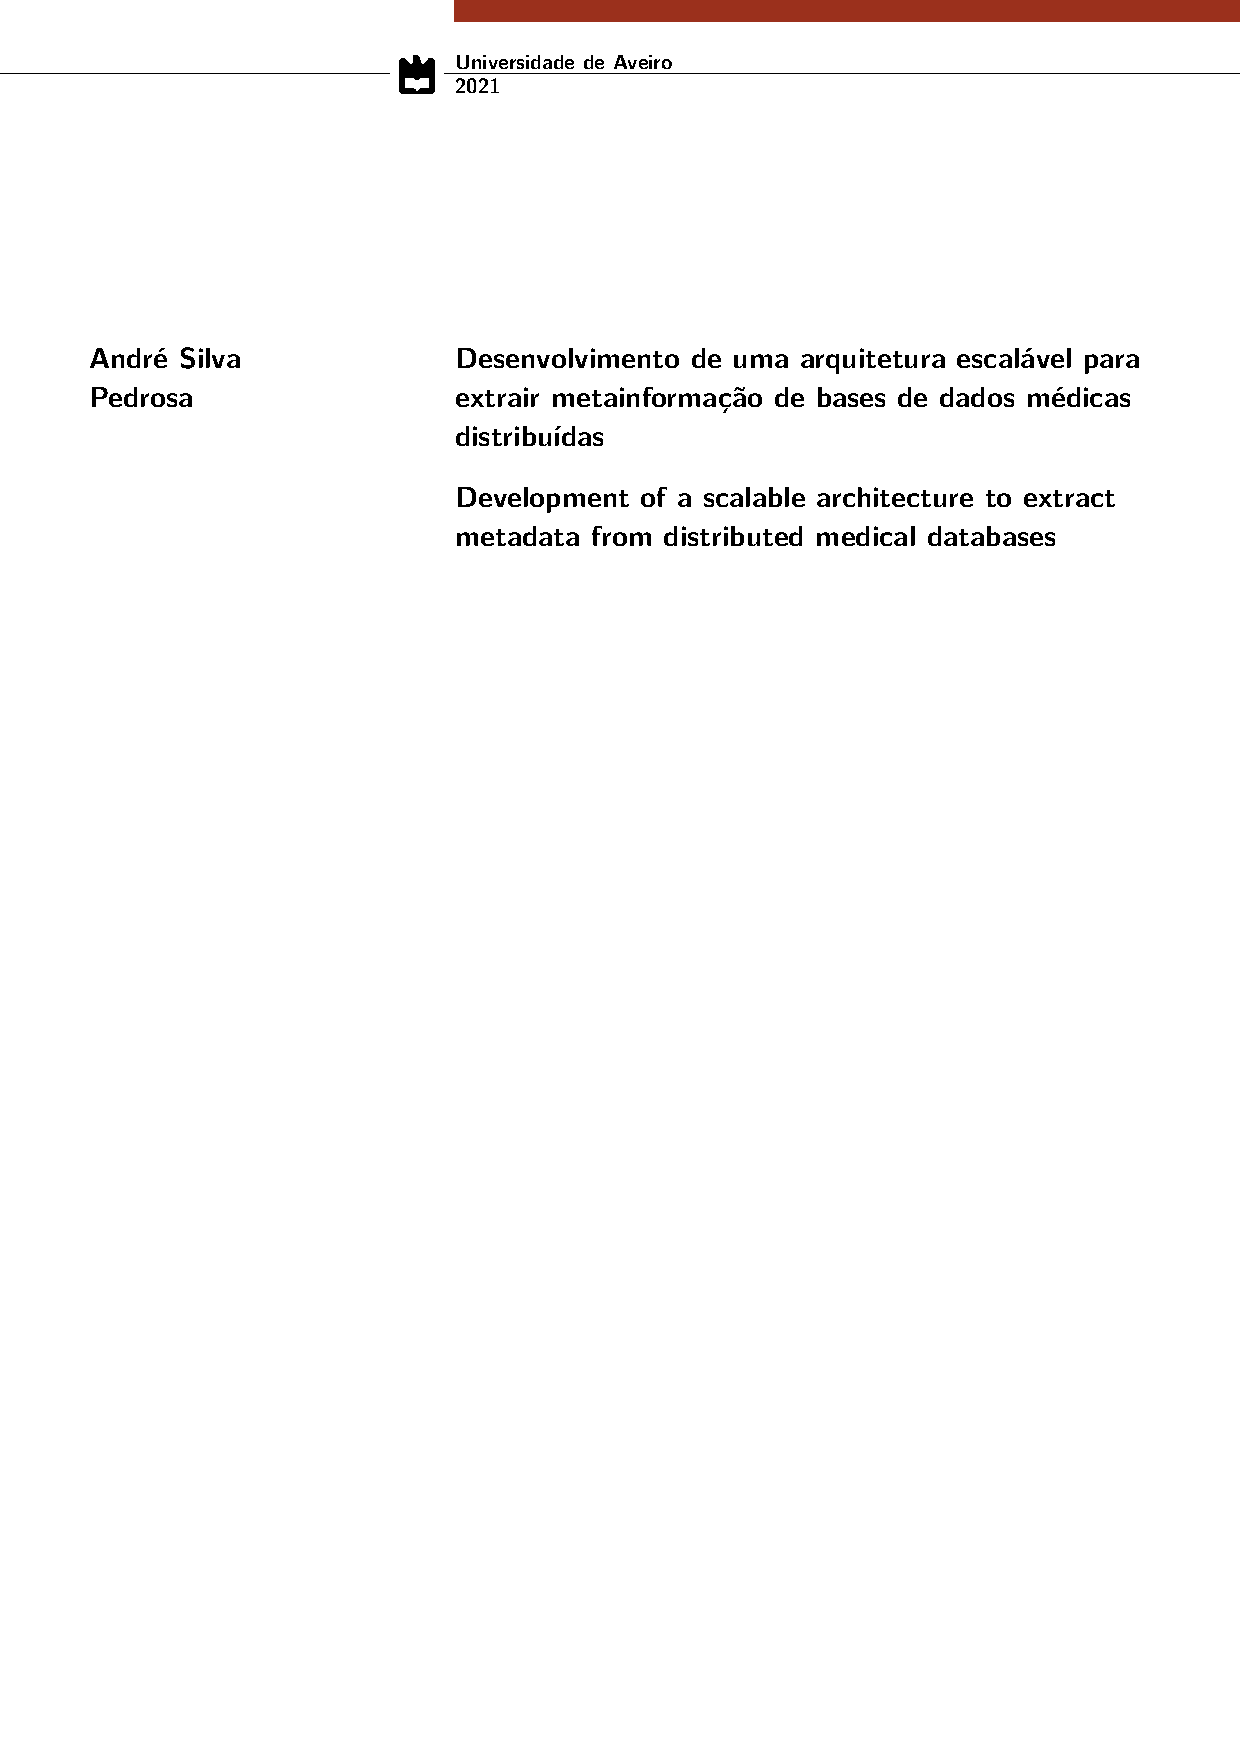
\includepdf[pages=-]{cover.pdf}

%
%Front matter

%Custom Chapter style named thesis
\makechapterstyle{thesis}{% Based on ell
  \chapterstyle{default}
  \renewcommand*{\chapnumfont}{\normalfont\sffamily}
  \renewcommand*{\chaptitlefont}{\normalfont\Huge\sffamily}
  \settowidth{\chapindent}{\chapnumfont 111}
  \renewcommand*{\chapterheadstart}{\begingroup
    \vspace*{\beforechapskip}%
    \begin{adjustwidth}{}{-\chapindent}%
    \hrulefill
    \smash{\rule{0.4pt}{15mm}}
    \end{adjustwidth}\endgroup}
  \renewcommand*{\printchaptername}{}
  \renewcommand*{\chapternamenum}{}
  \renewcommand*{\printchapternum}{%
    \begin{adjustwidth}{}{-\chapindent}
    \hfill
    \raisebox{10mm}[0pt][0pt]{\fontsize{30}{25}\selectfont\chapnumfont \thechapter}%
                              \hspace*{1em}
    \end{adjustwidth}\vspace*{-3.0\onelineskip}}
  \renewcommand*{\printchaptertitle}[1]{%
    \vskip\onelineskip
    \raggedleft {\chaptitlefont ##1}\par\nobreak\vskip 4\onelineskip}}


%Select chapter style from existing or select custom
%\chapterstyle{thesis} % Others: dowding, demo2, dash, chappell, brotherton, bianchi, ger, madsen, tatcher, veelo,indexes)
% thesis can also be used as defined previously
%

%If you feel adventurous you can also define all aspects of your theme
%Use either this input or the chapterstyle before
%% Rules
\newcommand{\thinRule}{\rule{\textwidth}{0.25pt}}

% Customize heading appearances
% Define styles
\newcommand{\partSize}{\Huge}
\newcommand{\partStyle}{\lsstyle\scshape}
\newcommand{\chapterSize}{\Huge}
\newcommand{\chapterStyle}{\lsstyle\scshape}
\newcommand{\chapterAfter}{}
\newcommand{\sectionSize}{\Large}
\newcommand{\sectionStyle}{\scshape\MakeTextLowercase}
\newcommand{\subsectionSize}{\large}
\newcommand{\subsectionStyle}{\scshape\MakeTextLowercase}
\newcommand{\subsubsectionSize}{\large}
\newcommand{\subsubsectionStyle}{\scshape\MakeTextLowercase}
\newlength{\partNumSizePt}
\setlength{\partNumSizePt}{60pt}
\newlength{\chapterNumSizePt}
\setlength{\chapterNumSizePt}{60pt}
\newcommand{\partNumSize}{%
  \fontsize{\partNumSizePt}{1.2\partNumSizePt}\selectfont%
}
\newcommand{\partNumStyle}{\partChapterNumColor}
\newcommand{\chapterNumSize}{%
  \fontsize{\chapterNumSizePt}{1.2\chapterNumSizePt}\selectfont%
}
\newcommand{\chapterNumStyle}{\partChapterNumColor}

% Customize parts
\renewcommand{\partnamefont}{\partSize\partStyle}
\renewcommand{\partnumfont}{\partNumSize\partNumStyle}
\renewcommand{\printpartname}{}
\renewcommand{\printparttitle}[1]{%
  \normalfont\normalcolor\partnamefont #1
}

% Customize chapters
\makeatletter
\setlength{\beforechapskip}{30pt}
\renewcommand*{\chapterheadstart}{\vspace*{\beforechapskip}}
\setlength{\afterchapskip}{3ex}
\setlength{\midchapskip}{3ex}
\renewcommand*{\chapnamefont}{%
  \Large\flushright\chapterStyle\partChapterNumColor%
}
\renewcommand*{\chapnumfont}{\chapterNumSize\chapterNumStyle}
\renewcommand*{\chaptitlefont}{%
  \normalfont\flushleft\normalcolor\chapterSize\chapterStyle%
}
\renewcommand*{\printchaptername}{%
  \chapnamefont\MakeTextLowercase{\@chapapp}%
}
\renewcommand*{\chapternamenum}{\quad}
\renewcommand*{\printchapternum}{%
%  \chapnumfont\textls[-75]{\classicstylenums{\thechapter}}%
 \chapnumfont\textls[-75]{\thechapter}%

}
\renewcommand*{\printchaptertitle}[1]{%
  \chaptitlefont #1
  \chapterAfter
}
\makeatother
% Customize sections and subsections
\setsecnumformat{\csname my#1\endcsname\quad}
\setsecheadstyle{\sectionSize\sectionStyle}
\newcommand{\mysection}{{\thesection}}
\setlength{\beforesecskip}{3em}


\setsubsecheadstyle{\subsectionSize\subsectionStyle}
\newcommand{\mysubsection}{{\normalfont\subsectionSize\thesubsection}}
\setlength{\beforesubsecskip}{3em}

\setsubsubsecheadstyle{\subsubsectionSize\subsubsectionStyle}
\newcommand{\mysubsubsection}{{\normalfont\subsubsectionSize\thesubsubsection}}
\setlength{\beforesubsubsecskip}{2em}

% Customize "Table of ..." appearance
% Customize headings
\newcommand{\renewPrintXTitle}[1]{%
  \renewcommand{#1}[1]{%
    \printchaptertitle{##1}%
  }%
}
\renewPrintXTitle{\printtoctitle}
\renewPrintXTitle{\printlottitle}
\renewPrintXTitle{\printloftitle}

% Customize ToC headings
\renewcommand{\cftpartfont}{\partChapterNumColor\partStyle}
\renewcommand{\cftchapterfont}{\chapterStyle}
\renewcommand{\cftsectionfont}{}
\renewcommand{\cftsubsectionfont}{}
\renewcommand{\cftfigurefont}{}
\renewcommand{\cfttablefont}{}
\newcommand{\cftlstlistingfont}{}

% Increase number width
\newlength{\cftNumWidthIncrease}
\setlength{\cftNumWidthIncrease}{0.25em}
\addtolength{\cftpartnumwidth}{\cftNumWidthIncrease}
\addtolength{\cftchapternumwidth}{\cftNumWidthIncrease}
\addtolength{\cftsectionindent}{\cftNumWidthIncrease}
\addtolength{\cftsubsectionindent}{\cftNumWidthIncrease}
% No leader dots
%\renewcommand*{\cftpartdotsep}{\cftnodots}
%\renewcommand*{\cftchapterdotsep}{\cftnodots}
%\renewcommand*{\cftsectiondotsep}{\cftnodots}
%\renewcommand*{\cftsubsectiondotsep}{\cftnodots}
%\renewcommand*{\cftfiguredotsep}{\cftnodots}
%\renewcommand*{\cfttabledotsep}{\cftnodots}
%\newcommand*{\cftlstlistingdotsep}{\cftnodots}
% Set page numbers immediately after entry text
\newcommand{\tocEntryPageSep}{\hspace{1em}}
\renewcommand{\cftpartleader}{\cftdotfill{\cftdotsep}}
%\renewcommand{\cftpartafterpnum}{\cftparfillskip}
%\renewcommand{\cftchapterleader}{\tocEntryPageSep}
\renewcommand{\cftchapterleader}{\cftdotfill{\cftdotsep}}
%\renewcommand{\cftchapterafterpnum}{\cftparfillskip}
\renewcommand{\cftsectionleader}{\cftdotfill{\cftdotsep}}
%\renewcommand{\cftsectionafterpnum}{\cftparfillskip}
\renewcommand{\cftsubsectionleader}{\cftdotfill{\cftdotsep}}
%\renewcommand{\cftsubsectionafterpnum}{\cftparfillskip}
\renewcommand{\cftfigureleader}{\cftdotfill{\cftdotsep}}
%\renewcommand{\cftfigureafterpnum}{\cftparfillskip}
\renewcommand{\cfttableleader}{\cftdotfill{\cftdotsep}}
%\renewcommand{\cfttableafterpnum}{\cftparfillskip}
\newcommand{\cftlstlistingleader}{\cftdotfill{\cftdotsep}}
%\newcommand{\cftlstlistingafterpnum}{\cftparfillskip}
% Customize page numbers
\newcommand{\tocPageStyle}{\tocPageColor}
\renewcommand{\cftpartpagefont}{\tocPageStyle}
\renewcommand{\cftchapterpagefont}{\tocPageStyle}
\renewcommand{\cftsectionpagefont}{\tocPageStyle}
\renewcommand{\cftsubsectionpagefont}{\tocPageStyle}
\renewcommand{\cftfigurepagefont}{\tocPageStyle}
\renewcommand{\cfttablepagefont}{\tocPageStyle}
\newcommand{\cftlstlistingpagefont}{\tocPageStyle}

% Abstract
% Remove indents around abstract text
\setlength{\absleftindent}{0pt}
\setlength{\absrightindent}{0pt}
% Change font size to conform with the rest of the document text
\renewcommand{\abstracttextfont}{\normalsize}

% Customize headers and footers including page numbers
\newcommand{\hfTextSize}{\footnotesize}
\newcommand{\headTextStyle}{\lsstyle\scshape\MakeTextLowercase}
\nouppercaseheads
\makeevenhead{headings}%
             {\hfTextSize\thepage}%
             {}%
             {\hfTextSize\headTextStyle\leftmark}
\makeevenhead{plain}%
             {\hfTextSize\thepage}%
             {}%
             {\hfTextSize\headTextStyle\leftmark}
\makeoddhead{headings}%
            {\hfTextSize\headTextStyle\rightmark}%
            {}%
            {\hfTextSize\thepage}
\makeoddhead{plain}%
            {\hfTextSize\headTextStyle\rightmark}%
            {}%
            {\hfTextSize\thepage}


% Customize captions
\newcommand{\captionSize}{\small}
\newcommand{\captionStyle}{\scshape}
\newcommand{\captionWidthRatio}{0.9}

\captionnamefont{\captionSize\captionStyle}
\captiontitlefont{\captionSize}
\captiondelim{ -- }
\captiontitlefinal{}
\changecaptionwidth
%\captionwidth{\captionWidthRatio\textwidth}

% Define colors
%\newcommand{\titleColor}{\color[rgb]{0.616, 0.0627, 0.176}}
\newcommand{\titleColor}{\color[rgb]{0,0,0}}

\newcommand{\partChapterNumColor}{\titleColor}
\newcommand{\dropCapColor}{\titleColor}
%\newcommand{\tocPageColor}{\color[rgb]{0.0980, 0.329, 0.651}}

\newcommand{\tocPageColor}{\color[rgb]{0, 0,0}}
\definecolor{shade0}{rgb}{1.0 , 1.0 , 1.0 }
\definecolor{shade1}{rgb}{0.9 , 0.9 , 0.9 }
\definecolor{shade2}{rgb}{0.8 , 0.8 , 0.8 }
\definecolor{shade3}{rgb}{0.65, 0.65, 0.65}
\definecolor{shade4}{rgb}{0.45, 0.45, 0.45}
\definecolor{shade5}{rgb}{0.0 , 0.0 , 0.0 }



\chapterstyle{veelo}
%Exclude sub figures from List of Figures
%\captionsetup[subfloat]{list=no}


% Texts
\newenvironment{introduction}
{%
  \begin{minipage}{\textwidth}%
   \itshape%
}
{%
  \end{minipage}%
  \par\addvspace{2\baselineskip plus 0.2\baselineskip minus 0.2\baselineskip}%
}


%Select Page style
\pagestyle{plain}

\frontmatter

\tightlists
\midsloppy
\raggedbottom

\setcounter{tocdepth}{2} %subsections are added to the TOC
\setcounter{secnumdepth}{4} %subsubsections are numbered


\cleardoublepage

%Table of contents
{\small\tableofcontents}
\cleardoublepage

%List of figures
%{\small\listoffigures}


%List of tables
%%\cleardoublepage
%%{\small\listoftables}

%Print Glossary
{\small \newacronym{ehden}{EHDEN}{European Health Data and Evidence Network}
\newacronym{ohdsi}{OHDSI}{Observational Health Data Sciences and Informatics}
\newacronym{eu}{EU}{European Union}
\newacronym{cdm}{CDM}{Common Data Model}
\newacronym{omop}{OMOP}{Observational Medical Outcomes Partnership}
\newacronym{fair}{FAIR}{Findability, Accessibility, Interoperability, and Reusability}
\newacronym{api}{API}{Application Programmable Interface}
\newacronym{redcap}{REDCap}{Research Electronic Data Capture}
\newacronym{gaain}{GAAIN}{Global Alzheimer's Association Interactive Network}
\newacronym{dpc}{DPC}{Data Partner Clients}
\newacronym{bbmri-eric}{BBMRI-ERIC}{Biobanking and BioMolecular Resources Research Infrastructure-European Research
Infrastructure Consortium}
\newacronym{rd}{RD}{Research and Development}
\newacronym{achilles}{ACHILLES}{Automated Characterization of Health Information at Large-scale Longitudinal Evidence Systems}
\newacronym{emif}{EMIF}{European Medical Information Framework}
\newacronym{pds}{PDS}{Project Data Sphere}
\newacronym{nada}{NADA}{National Data Archive}
\newacronym{json}{JSON}{JavaScript Object Notation}
\newacronym{dats}{DATS}{DatA Tag Suite}
\newacronym{ehr}{EHR}{Electronic Health Record}
\newacronym{cdw}{CDW}{Clinical Data Warehouse}
\newacronym{crud}{CRUD}{Create, Read, Update and Delete}
\newacronym{xss}{XSS}{Cross-Site Scripting}
\newacronym{html}{HTML}{HyperText Markup Language}
\newacronym{orm}{ORM}{Object–Relational Mapping}
\newacronym{sql}{SQL}{Structured Query Language}
\newacronym{http}{HTTP}{HyperText Transfer Protocol}
\newacronym{ide}{IDE}{Integrated Development Environment}
\newacronym{cdn}{CDN}{Content Delivery Network}
\newacronym{npm}{NPM}{Node Package Manager}
\newacronym{rest}{REST}{Representational State Transfer}
\newacronym{csv}{CSV}{Comma-separated values}
\newacronym{rdbms}{RDBMS}{Relational Database Management System}
\newacronym{amqp}{AMQP}{Advanced Message Queuing Protocol}
\newacronym{jms}{JMS}{Java Message Service}
}


%
%Main document starts here
%
\mainmatter



% Start of Thesis text ----------------------------------------------------------
%Line spacing: 1.5 pt
\OnehalfSpacing

%\chapter{Introduction}
\label{chapter:introduction}

Oftentimes medical researchers do studies associated with diseases, such as determining the impact of a certain drug or find variables that are characteristic of certain diseases.
To perform such studies and have reliable results, a great amount of data is required.
To obtain that data, these researchers have to contact medical data owners to have access to relevant data that can help improve their analysis and/or findings.

With this procedure emerges several problems for the researcher such as he has to find
institutions willing to share data and the process of contacting the data providers can
be cumbersome.
To aid in this whole process, several data hubs have been developed with the purpose of
making the process of data discovery easier.
One important aspect of such data hubs is that they present to the researcher meta
data, which is aggregations or summaries of the original data.
Metadata has the advantage that one doesn't have to deal with the anonymization process
of medical records, since only summaries of the initial data are retrieved
~\cite{egenvar, montra}.
With this dependency on the original data, emerges an important problem of data hubs
which is, metadata can easily be outdated after a small time window.
This could not raise a big problem, if the records were updated regularly, however this
rarely happens, mainly because either the update process is difficult or because
metadata has to be manually extracted and uploaded to the data hub.
A problem that still might arise from such platforms, is those different datasets very
often have different representation for the same concept or the data is organized in a
different layout.
The research is then hampered since either different approaches have to be taken to
analyze each dataset.

The \gls{ehden}~\cite{ehden} project has affiliations with several institutions, data sources and data custodians across the \gls{eu}, which the main goal is to, within a federated network~\cite{ehden-datapartners}, harmonize their data to the \gls{omop} \gls{cdm}, which was developed by \gls{ohdsi}, a multi-stakeholder, interdisciplinary and collaborative organization that brings out the value of health data through large-scale analytics~\cite{ohdsi-site}.
With a \gls{cdm}, the problem of having different representations for the same data
across distinct data sources is solved.
Researchers can now develop a single analysis method and then apply it to all gathered
datasets and these methods can be optimized for this specific data model, which allows
large-scale analytics.
Furthermore, also improves collaborative research~\cite{ohdsi-site}.
Still, within the scope of the \gls{ehden} project, the project has a database catalog~\cite{ehden-portal},
built with the MONTRA framework~\cite{montra}, where data owners fill metadata about
their data source manually, which brings the outdated problem already mentioned before.
Additionally, whenever new metadata fields are introduced, the data owners of all data
sources have to go manually update their metadata form.

\section{Objectives}
The purpose of this dissertation is to create a system that can automate the update process of metadata stored in online platforms, that aids in the procedure of finding the correct data set for a specific study.
Such a system must be able to extract metadata from the databases, for that, an agent software will be installed along with each databases' local system.
Additionally, as new software components might be developed, it is a great opportunity to try new technologies.

With that, the following goals were established:
\begin{itemize}
    \item have a platform capable of holding and displaying metadata in an intuitive and user-friendly way;
    \item develop or find a tool that extracts metadata from a database;
    \item design a system capable of sending data to an application, to keep their data up-to-date;
    \item make use of new technologies with growing popularity.
\end{itemize}

\section{Outline}
This dissertation is organized into five more chapters, which are described below.

Chapter \ref{chapter:background} intends to provide a state-of-the-art characterization associated with the work of the dissertation.
Regarding the several goals established, several solutions and approaches were studied.

In chapter \ref{chapter:metadata-visualization} a software framework used to develop platforms to store and visualize metadata is described.
Has this framework had some design flaws, the chapter also details all the improvements performed.

Chapter \ref{chapter:extraction-update} describes the entire development process around the tool to extract metadata and the metadata management system that automates the update process of metadata.
It starts by detailing all the requirements associated with such components, then describes both the architecture and implementation of both the extraction tool and the metadata management system.

The Chapter \ref{chapter:evalution} is used to show the integration of all the components developed in the previous chapters.

The last chapter, \ref{chapter:conclusion}, presents the main achievements with the work, main challenges found and future work.

%\chapter{Background}
\label{chapter:background}

From a medical standpoint, to perform their studies, researches need to contact data
owners to have access to relevant data that can help improve their analysis and/or
findings that can be applied to real cases.
With this procedure emerges several problems for the researcher such as he has to find
institutions willing to share data and the process of contacting the data providers can
be cumbersome.
To aid in this whole process, several data hubs have been developed with the purpose of
making the process of data discovery easier.
One important aspect of such data hubs is that they present to the researcher meta
data, which is aggregations or summaries of the original data.
Metadata has the advantage that one doesn't have to deal with the anonymization process
of medical records, since only summaries of the initial data are retrieved
\cite{egenvar, montra}.
With this dependency on the original data, emerges an important problem of data hubs
which is, metadata can easily be outdated after a small time window.
This could not raise a big problem, if the records were updated regularly, however this
rarely happens, mainly because either the update process is difficult or because
metadata has to be manually extracted and uploaded to the data hub.
A problem that still might arise from such platforms, is those different datasets very
often have different representation for the same concept or the data is organized in a
different layout.
The research is then hampered since either different approaches have to be taken to
analyze each dataset.

The \gls{ehden} project has affiliations with several institutions, data sources and
data custodians across the \gls{eu}, which the main goal is to, within a federated
network, harmonize their data to the \gls{omop} \gls{cdm}\cite{ehden-datapartners}.
With a \gls{cdm}, the problem of having different representations for the same data
across distinct data sources is solved.
Researchers can now develop a single analysis method and then apply it to all gathered
datasets and these methods can be optimized for this specific data model, which allows
large-scale analytics.
Furthermore, also improves collaborative research \cite{ohdsi-site}.
Still, within the scope of the \gls{ehden} project, the project has a database catalog,
built with the Montra framework \cite{montra}, where data owners fill metadata about
their data source manually, which brings the outdated problem already mentioned before.
Additionally, whenever new metadata fields are introduced, the data owners of all data
sources have to go manually update their metadata form.

To build a valuable data hub is then important to take into account how to:
\begin{itemize}
    \item extract metadata from a data source
    \item upload and update the metadata on the data hub
    \item automatize the two processes mentioned before
    \item receive and display the metadata on the data hub in a way that facilitates
        readability.
\end{itemize}

\section{Metadata visualization tools}
It will then be explored existing visualization platforms that enhance data discovery
by presenting summaries or metadata of records (data sources, datasets).

In some cases data can't be publicly available because it contains sensitive data or
simply the data owner might not want to share some portions of the data, for that the
tools analyzed should have privacy protection mechanisms, allowing to customize the
access and manipulation of data stored.

Furthermore, considering we want to improve and assist data discovery and reuse it is
important to have good data management to simplify such processes.
However, humans fail to achieve the necessary processing levels with present-day
scientific data.
It is then important that data is provided in such a way that machines can fetch,
understand, analyze and act on data.
For that the \gls{fair} Guiding Principles were established which contain a series of
considerations for data publishing to supports both human and machine operations such
as deposition, exploration, sharing and reuse \cite{fair}.

Finally, it is preferential for such a tool to be open source since the available
solution might need some changes to solve our specific problem, and also it makes it
possible to receive contributions from the community.

\subsection{Search Method}

Regarding this subject, there was already done a systematic review of several tools
that fit within the current search pool.
Its objective was to "identify projects and software solutions that promote patient
electronic health data discovery, as enablers for data reuse and advancement of
biomedical and translational research" \cite{systematic_review}.
From the final 20 systems, they captured their interoperability, what type of data they
were providing and their after effect related to scientific results and improvements to
better healthcare.
To perform their search they only used PubMed
\footnote{https://pubmed.ncbi.nlm.nih.gov/} considering it indexes a substantially
amount of health-care related work and provides a public \gls{api} which allows
automation of the retrieval process.
The programmatic retrieval was done using the Biopython
framework\footnote{https://biopython.org/} where all search queries were limited to the
time windows between January 2014 to September 2018.

A softer version of the previous systematic review was done now within November 2018
and December 2020.
Also, instead of doing a query to PubMed and then find related publications, the
process taken here was to skip the first step and find related publications of the
final 20 selected on the systematic review and then try to find some software solutions
of interest.

\subsection{Findings}

From the systematic review mentioned before, only software solutions were considered
and projects were excluded.

\begin{tabular}{ | c | c | c | c | c | }
\hline 
Tool Name & Open Source & \makecell{Warehouse \\ vs \\ Owner's site}  & Data & FAIR\\
\hline
REDCap \cite{redcap} & No & Warehouse & -- & -- \\
\hline
Vanderbilt \cite{vanderbilt} & -- & Warehouse & -- & -- \\
\hline
Data Sphere \cite{datasphere} & -- & Warehouse & -- & -- \\
\hline
BBMRI-ERIC \cite{bbmrieric} & -- & Warehouse & -- & -- \\
\hline
Brain-CODE \cite{braincode} & Yes & Warehouse & -- & -- \\
\hline
B-CAN \cite{bcan} & -- & Warehouse & -- & -- \\
\hline
RD-Connect \cite{rdconnect} & -- & Warehouse & -- & Yes \\
%\hline
%CoMetaR \cite{cometar} & -- & Warehouse & -- & -- \\
\hline
\makecell{Global Alzheimer's \\Association Interactive\\ Network} \cite{gaain} & -- & Warehouse & -- & -- \\
\hline
Cafe Variome \cite{cafevariome} & No & Both & -- & -- \\
\hline
MONTRA \cite{montra} & Yes & Warehouse & -- & -- \\
\hline
Harvest \cite{harvest} & Yes & Warehouse & -- & -- \\
\hline
eGenVar \cite{egenvar} & -- & Warehouse & -- & -- \\
\hline
PopMedNet \cite{popmednet} & -- & Warehouse & -- & -- \\
\hline
Cataloguing toolkit by Maelstrom \cite{maelstrom} & Yes & Warehouse & -- & -- \\
\hline
DataMed \cite{datamed} & Yes & -- & -- & -- \\
\hline
EHR4CR \cite{ehr4cr} & -- & -- & -- & -- \\
\hline
YummyData \cite{yummydata} & Yes & Warehouse & -- & Yes \\
\hline
BioSharing \cite{biosharing} & -- & -- & -- & -- \\
\hline
Open PHACTS \cite{phacts} & -- & -- & -- & -- \\
\hline
\end{tabular}

\section{Fingerprinting Tools}

OMOP CDM
OHDSI TOOLS 

ACHILLES

https://github.com/EHDEN/CatalogueExport

\section{Network of Fingerprinting agents}

\chapter{Metadata Visualization}
\label{chapter:metadata-visualization}
\graphicspath{{figs/03-visualization/}}

Among the presented tools in chapter \ref{chapter:background}, MONTRA was our go-to mainly because of its data source-centric approach.
Also, no real data is shown here, only metadata is handled within the platform.
Yet, it still allows imposing access permissions at several levels.

This chapter will detail the crucial concepts of the MONTRA framework and its internal data model, followed by the description of the refactoring process that was done to the platform, with improvements and its flaws fixed.

\section{MONTRA}
% O que é o montra e o seu estado atual
% explicar de maneira mais aprefundada a paltaforma, realçando partes que devem ser alteradas ou que não estão corretas

Originally, the MONTRA framework was developed by the Bioinformatics team of the Institute of Electronics and Informatics Engineering of Aveiro associated with the \gls{emif} project with the goal to develop a common patient health information framework with emphasis on the research topics of Obesity and its metabolic complications and Markers for the development of Alzheimer's disease and other dementias.
The code is publicly available on github\footnote{https://github.com/bioinformatics-ua/montra}, whereby Django 1.4, a high-level Python Web framework\cite{django}, was used as a framework to develop the entire system.
This framework allows to develop complete web applications, in a faster and easier way.
It contains a model layer that allows specifying database tables through python classes called models, following a \gls{orm} approach, allowing to perform database queries through python code instead of \gls{sql} queries.
Django can then check if there are new models or if existing ones have changed. Such changes are then expressed through database migration files which will apply them to the database tables.
Next, the developer can set custom URL patterns so specific requests are handled by a specific function of the view layer, where the business logic will be implemented.
Finally, Django contains a template layer that allows building dynamic \gls{html} pages without requiring to have a separate javascript framework to do such.
The developer builds the main static structure of the page and then uses a special syntax that describes how Django should display the data received from the view layer.
Django also has an important form feature that allows to easily create a set of pages that allow performing the usual \gls{crud} operation over the database model.

MONTRA's development started at the beginning of 2013 and ended in the middle of 2018.
After this, at the end of 2018, the framework was adopted by the \gls{ehden} project, to develop a portal to allow discovery and analysis of health data on their network of data sources.
Currently, the project is being developed in a private repository but intends to make it public after the code base is more robust and well documented.

\subsection{Communities}

In the first versions of the framework, MONTRA allowed only one level of organization related to data sources, in which they could only be separated according to their skeleton that describe their original data, which will be more detailed in the next subsection.
Newer versions created the concept of a Community.
This allows having multiple networks of data sources on the same portal, where originally the only option was to have different installations of the framework.

These communities can be created in several ways:

\begin{enumerate}
    \item the admin can create it through Django's admin console;
    \item a user can request a community to be created through a form and then the admin will receive an admin with such request;
    \item the MONTRA installation can be deployed in a single community mode where only one community exists, which is created on the first setup, giving the idea that there is no community concept on the platform.
\end{enumerate}

They also can have different access levels:

\begin{itemize}
    \item Open: Does not require membership. Any user can access the data sources of this community;
    \item Public: Does not require a membership however, the user needs to accept a set of terms and conditions before being able to access the data sources;
    \item Moderated: A user has to request the community managers for approval;
    \item Invitation: Users can only access and see the community by invite and subsequent approval.
\end{itemize}

\subsection*{Plugins}
The concept of Community also allows customization at that level, affecting only sections within that given community.
One example of such customization is plugins, a way to extend the functionalities of the framework without having to deal with the base code.
These plugins can either be full web applications, with different functionalities, that are linked to MONTRA through the community navigation menu or extensions that provide extra data services such as a dashboard about the data of a data source.

\subsection{Questionnaires}
% questions
% tipo de questoes

As the data from different data sources is highly heterogeneous, MONTRA ensures that the data inserted within a given community follow a common structure.
This structure is called a skeleton, which is represented in a form of a questionnaire with a set of questions, which can then be grouped in sections called Question Sets.
It represents a set of metadata that better describes the original data of data sources that need to remain private.
The skeleton schema can easily be defined through a spreadsheet, which will be more detailed on subsection \ref{subsection:excel}.

Next is presented the available question types which can be used to build a questionnaire for a community

\begin{longtable}[c]{|c|c|}
\hline
\textbf{Type}                     & \textbf{Description}                                        \\ \hline
\endhead
choice                            & Single choice (radio box)                                   \\ \hline
choice-freeform                   & Single choice with an open text fields                      \\ \hline
choice-multiple                   & Multiple choice (checkbox)                                  \\ \hline
choice-multiple-freeform          & Multiple choice with and open text fields                   \\ \hline
choice-multiple-freeform-options  & Multiple choice with and open text fields                   \\ \hline
choice-tabular                    & Creates a table with single, multiple choices or text by row      \\ \hline
choice-yesno                      & Single choice with yea and no choices                       \\ \hline
choice-yesnodontknow              & Single choice with yes, no and do not know choices          \\ \hline
comment                           & Used to separate groups of questions                        \\ \hline
custom                            & Mirrors another question by its type                        \\ \hline
datepicker                        & Field with date picker widget                               \\ \hline
email                             & Text input with email validation                            \\ \hline
%location                          & Set of select elements to choose a location                 \\ \hline
numeric                           & Numeric input                                               \\ \hline
open                              & Text field with no validation                               \\ \hline
open-button                       & Text input with backend validation                          \\ \hline
open-location                     & Text input with autocomplete sugestions                     \\ \hline
open-multiple                     & Allows to record an history of a value overtime             \\ \hline
open-multiple-composition         & Allows to record an history of several values overtime      \\ \hline
open-textfield                    & Same as open but a textarea html tag is used                \\ \hline
open-upload-image                 & Image upload                                                \\ \hline
open-validated                    & Text input with a regex validation                          \\ \hline
publication                       & A custom widget that allows to attach a set of publications \\ \hline
%range                             & Allows to define a range of numeric values                  \\ \hline
sameas                            & Mirrors another question by its number                      \\ \hline
timeperiod                        & Numeric input + select to choose numeric unit               \\ \hline
url                               & Text input with url validation                              \\ \hline
\caption{All available question types that can be used to build a questionnaire.}
\label{tab:original-question-types}\\
\end{longtable}

\subsection{Fingerprints}
\label{sec:fingerprints}
% Views
% validação feita toda do lado do cliente, existindo a possiblidade de ataques xss
% a validação builtin do django não está a ser usada

A fingerprint is a name given to the set of answers to the questionnaire.
In other words, it is the metadata that betters describes the original data source.
Data owners can start to answer the questions to build the profile of their data sources once there are communities on the platform and, these have at least a questionnaire associated.

On the list presented in figure \ref{fig:listings}, we can notice that the only fingerprint present is marked as draft.
This is a state of the fingerprint which prevents from non-ready or non-approved fingerprints will not show to the regular community users.
With this, for such users the list showed above would be empty.
Fingerprints can be published depending on the chosen settings for the community.
After the data source owners request to publish a fingerprint the framework allows to either automatically accept or require a community manger to accept it.

\begin{figure}[H]
    \center
    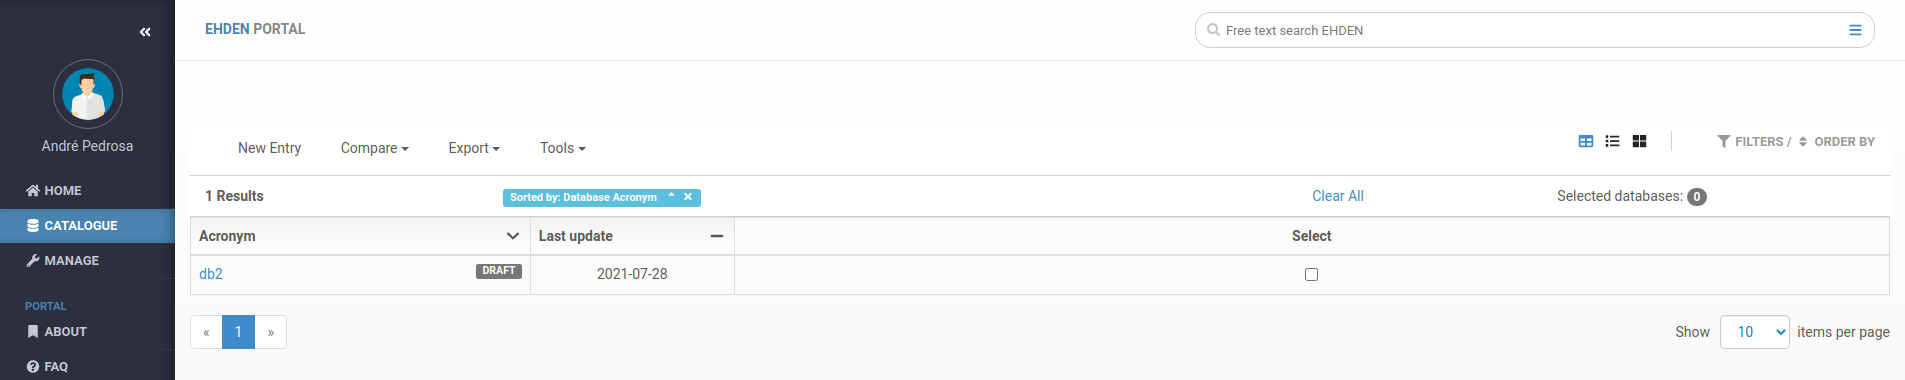
\includegraphics[width=\textwidth]{listings}
    \caption{The user interface displayed after selecting a community, which shows the list of the fingerprints of the chosen community.}
    \label{fig:listings}
\end{figure}

\subsection*{Views}

In figure \ref{fig:fingerprint-new} it is presented the user interface where a data owner can answer the questions of a questionnaire.
Each question of the questionnaire is placed under a container that can be collapsed, as is shown for question \textit{Instituition name}.
However, if multiple questions are grouped, the collapsable container will affect all questions of the group.

\begin{figure}[H]
    \center
    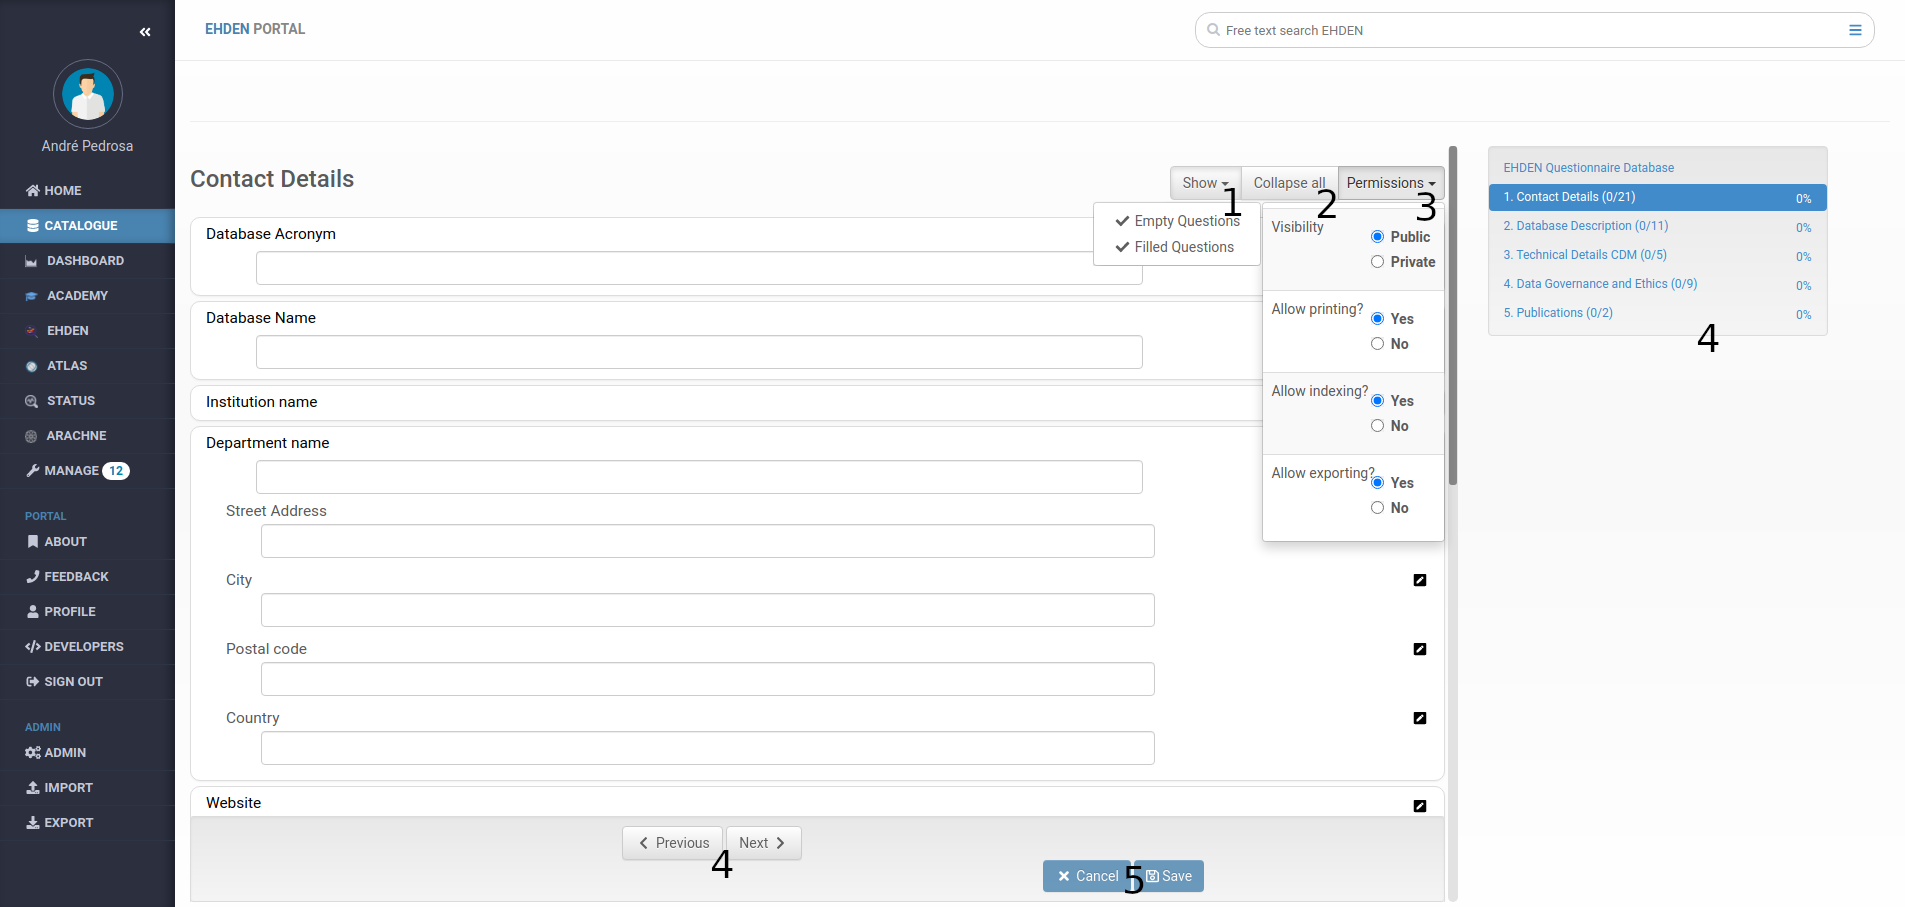
\includegraphics[width=\textwidth]{fingerprint-new}
    \caption{User interface to create a fingerprint.}
    \label{fig:fingerprint-new}
\end{figure}

Besides the input widget where the data owner can insert its answers, the user also has some additional control buttons:

\begin{enumerate}
    \item Allows to Hide or Show Questions that have been answered or that are empty. Besides being an interesting feature is important to note that on the last version it does not work, as clicking on the presented options will result in no visual effect;
    \item Allows to collapse or expand all questions or question groups containers;
    \item Allows the data owners to set permissions at the question set level;
        \begin{itemize}
            \item Visibility: Let plugins have access to answers data;
            \item Allow printing: On the fingerprints list page, showed in figure \ref{fig:listings}, there is a dropdown with tools, being the only one the "Print" tool (figure \ref{fig:listings-tools}). However, this feature is not correctly implemented since it calls the browser's built-int printing function on the fingerprint list page, so no actual fingerprint data will be printed. This permission ends up being useless. Additionally, if a user calls the browser's print function (e.g. hitting Ctrl+P) when viewing the data of a fingerprint, the platform will not block the action;
                \begin{figure}[H]
                    \center
                    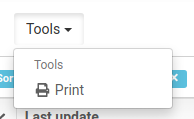
\includegraphics[width=.2\linewidth]{listings-tools}
                    \caption{Available tools on the fingerprint selection.}
                    \label{fig:listings-tools}
                \end{figure}
            \item Allow indexing: If the data owner allows indexing of the answers, which will allow for other users to find fingerprints based on the answers to a question of this specific question set;
            \item Allow exporting: If the answers to this question set can be included on the export file of a fingerprint.
        \end{itemize}
    \item Enable navigation along the question sets of the current questionnaire;
    \item Permits to save or cancel all the changes made to the current question set.
\end{enumerate}

Once the fingerprint is filled and published, a regular user can consult the metadata, which will be displayed by default in detailed view (figure \ref{fig:fingerprint-show-detailed}).
Similar to the create view, it is presented with some control buttons:

\begin{enumerate}
    \item Database level plugins associated with this community;
    \item Statistics of this fingerprint:
        \begin{itemize}
            \item Progress bar + Filled: How many questions of the questionnaire were answered;
            \item Hits: Number of times this fingerprint showed up on search queries;
            \item Unique Views: Number of users that visited this fingerprint.
        \end{itemize}
    \item Question set controls:
        \begin{itemize}
            \item Summary: Allows to switch to the summary view (Figure \ref{fig:fingerprint-show-summary});
            \item Collapse \& Show: The same role as mentioned for the create view.
        \end{itemize}
    \item Fingerprint control buttons:
        \begin{itemize}
            \item Subscribe: Receive notifications whenever changes are made to the fingerprint answers;
            \item Manage: Several fingerprint operations:
                \begin{itemize}
                    \item Edit: Enter the edit mode;
                    \item Share: Allows to add other users as owners of the fingerprint and also to create links that enable anonymous users to consult the fingerprint;
                    \item Export: Different forms of export. CSV, PDF, and MONTRA format to import on other installations of the MONTRA framework;
                    \item Delete: Remove the fingerprint from the community.
                \end{itemize}
        \end{itemize}
\end{enumerate}

\begin{figure}[H]
    \center
    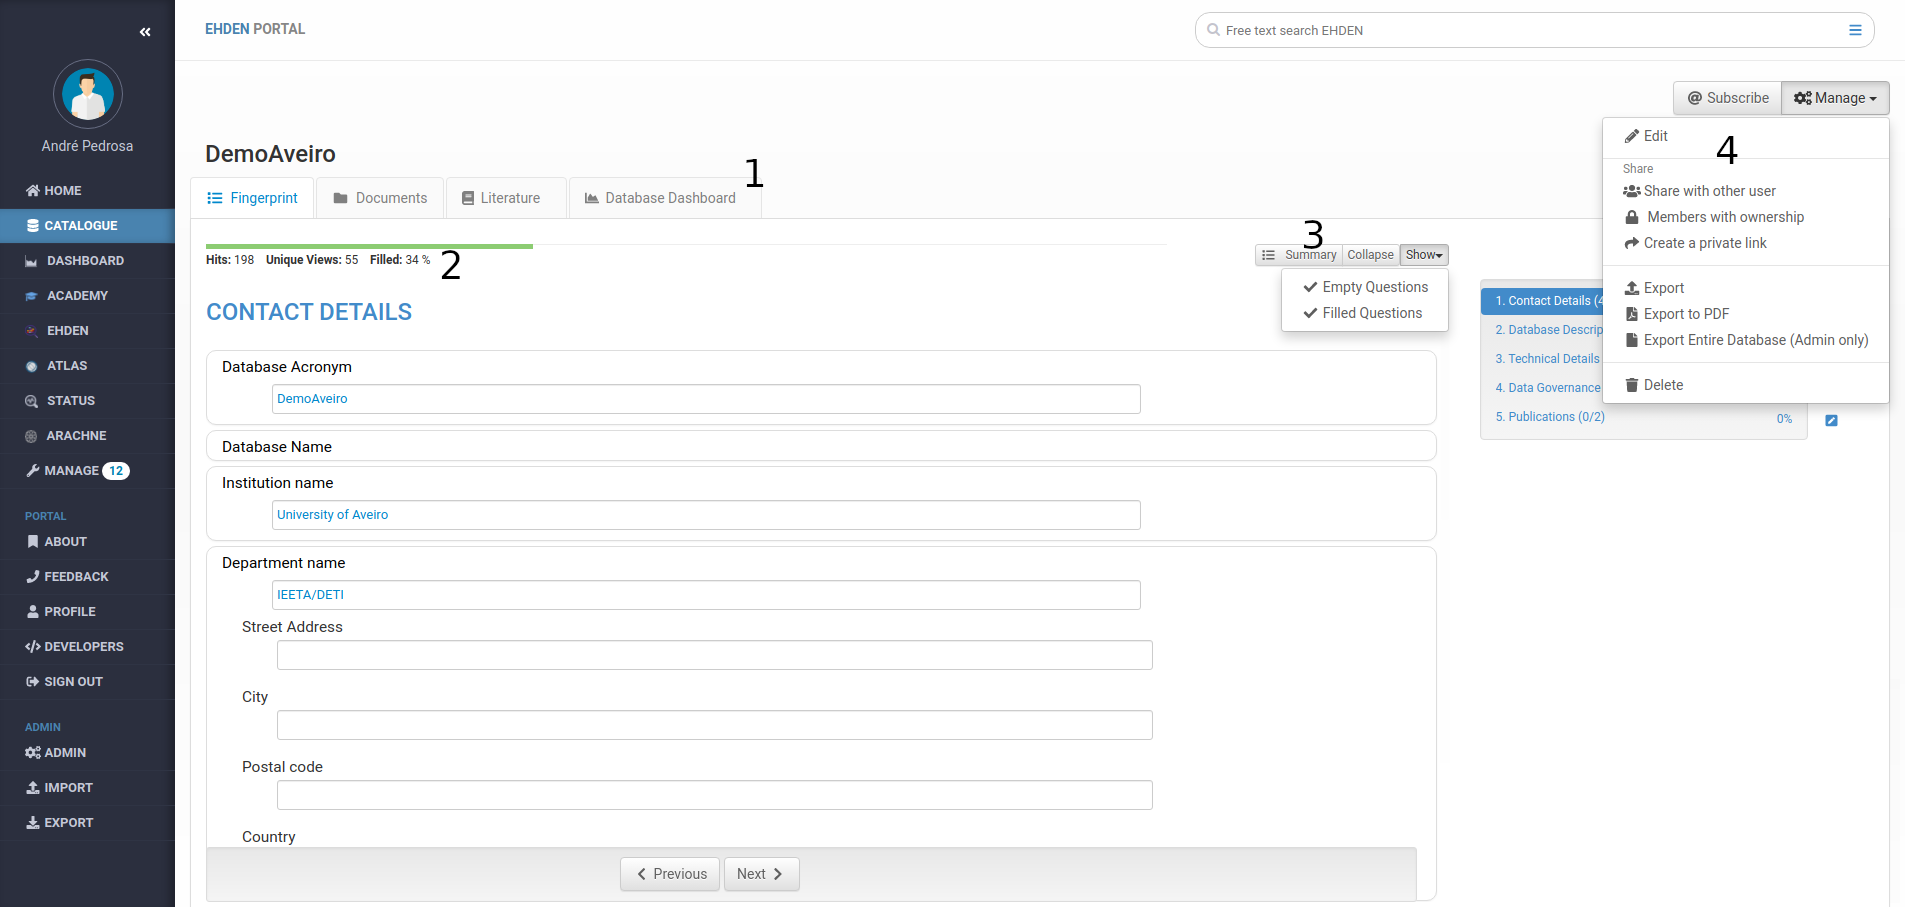
\includegraphics[width=\textwidth]{fingerprint-show-detailed}
    \caption{The detailed version of the interface to view and analyze fingerprints.}
    \label{fig:fingerprint-show-detailed}
\end{figure}

On the show view, if the user enters the summary view (Figure \ref{fig:fingerprint-show-summary}), the user is presented with a table with three columns where each row contains the question number, name and the answer given.
On this view, by hovering over an empty answer container the user can send a request to the database owner to answer the specific question.

\begin{figure}
    \center
    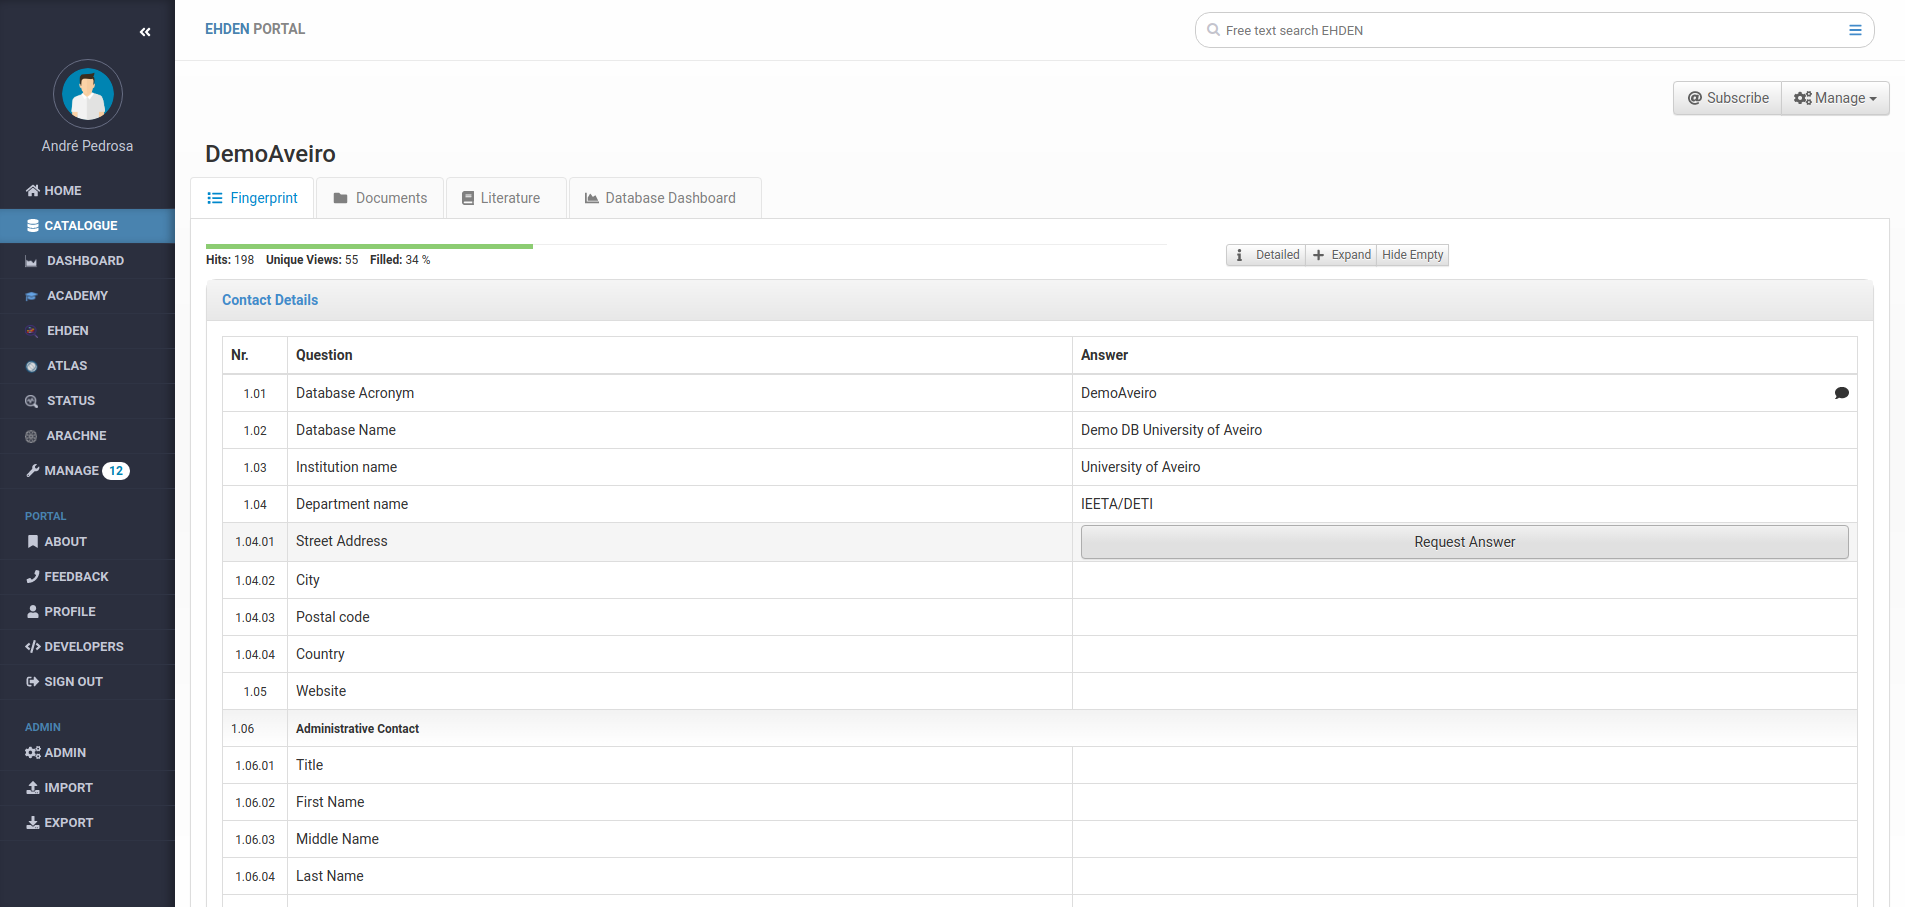
\includegraphics[width=\textwidth]{fingerprint-show-summary}
    \caption{The summary version of the interface to view and analyze fingerprints.}
    \label{fig:fingerprint-show-summary}
\end{figure}

The MONTRA framework also offers an ``Advanced Search'' feature, allowing to perform searches for fingerprints.
The overall interface used is identical to the ones presented above, where the user answers the questions of the specific questionnaire of the community.
The main difference to the other versions of the fingerprint view is that the only control buttons available are just the navigation ones, and all the questions do not have any validation.
Additionally, at the bottom of the page, it is provided to the user a way to customize the search query, allowing to create complex search criteria through a drag and drop interface, as is presented in figure \ref{fig:boolean-query}.

\begin{figure}[H]
    \center
    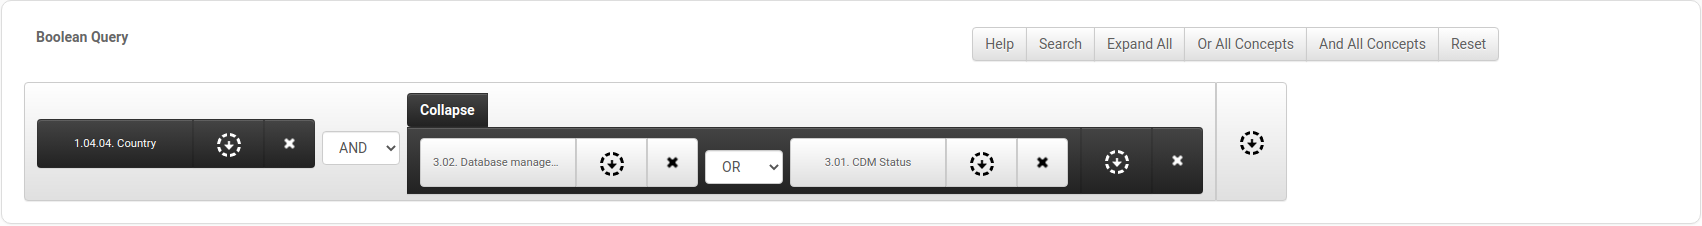
\includegraphics[width=\textwidth]{boolean-query}
    \caption{Interface to customize the search query.}
    \label{fig:boolean-query}
\end{figure}

% ---

Despite all these variations of the same view having a similar look, as some components appear on several variants, all views have a separate Django template, so there is some duplicated code across the different views.
If some changes are made to a shared component, such as the side question set menu bar, those changes have to be applied to all different templates.
This can be avoided since the Django template system allows to both include a shared component into other templates and also supports conditional rendering, for example, the permissions dropdown for a question set of a fingerprint should only be rendered when the user is editing or creating a fingerprint.

% ---

These different view versions provide a valid workflow to perform \gls{crud} operations over the metadata related to a data source, however, views that are used to insert or edit metadata of a fingerprint present several flaws related to how the inputs are validated and how they are presented to the user.

First, the validation of the user input is done on the client-side through javascript code that runs after a user submits a question set form.
Subsequently, the data is sent to the backend through \gls{api} calls.
However, if one would use the \gls{api} directly to update metadata of the fingerprint, the validation could be skipped and invalid data could be stored on the database.
In some cases there might exist some validation code on the server-side, however, this brings the necessity to maintain two separate code files.

Second, there is no escaping procedure done to the user's input when it is fetched from the database which allows that \gls{xss} attacks can be easily performed and put users that consult a compromised fingerprint at risk.
As an example, on figure \ref{fig:montra-xss-create} on the Database Name field, I added a \textit{script} tag with code that shows a popup and also a valid database name after.
Once a user opens the fingerprint to check the data, the code will execute, but the dummy name will render on the Database Name field, as seen in figure \ref{fig:montra-xss}.
This can be further exploited, where the user visiting the fingerprint will not notice that malicious code was executed.

\begin{figure}[H]
    \center
    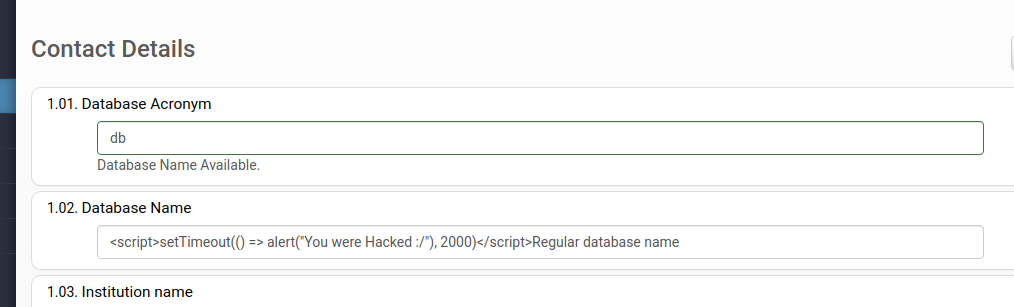
\includegraphics[width=0.75\textwidth]{montra-xss-create}
    \caption{Example of how an \gls{xss} attack could be done on MONTRA.}
    \label{fig:montra-xss-create}
\end{figure}

\begin{figure}[H]
    \center
    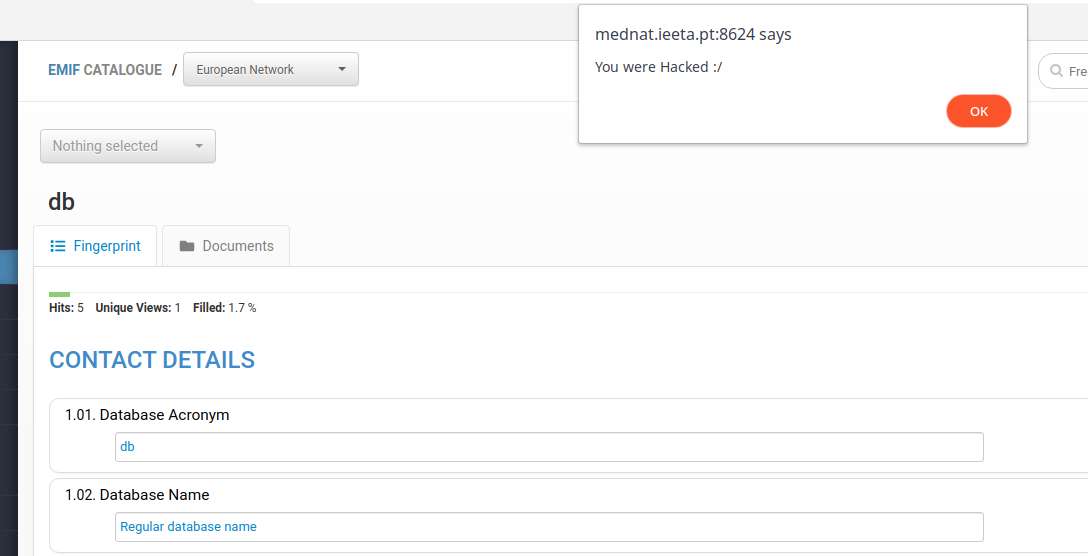
\includegraphics[width=0.75\textwidth]{montra-xss}
    \caption{Victim of a simple \gls{xss} attack.}
    \label{fig:montra-xss}
\end{figure}

All these problems exist because such views were developed from scratch without using the provided features that Django has out of the box for form validation and security.
For client-side validation, Django takes advantage of HTML5 form validation features~\cite{form-validation}.
This allows imposing restrictions and validations on the user's input without writing any additional javascript code.

To show these features I wrote a simple HTML file with a simple form that expects a number under 100 and an email.

\begin{verbatim}
<html>
  <body>
    <form>
      <label for"num">Number:</label>
      <input id="num" type="number" max="100">

      <label for"mail">Email:</label>
      <input id="mail" type="email">

      <button type="submit">Submit</button>
    </form>
  </body>
</html>
\end{verbatim}

If I try to submit the form with invalid values, error messages are presented as shown in figure \ref{fig:html-form-validation}.

\begin{figure}[H]
    \center
    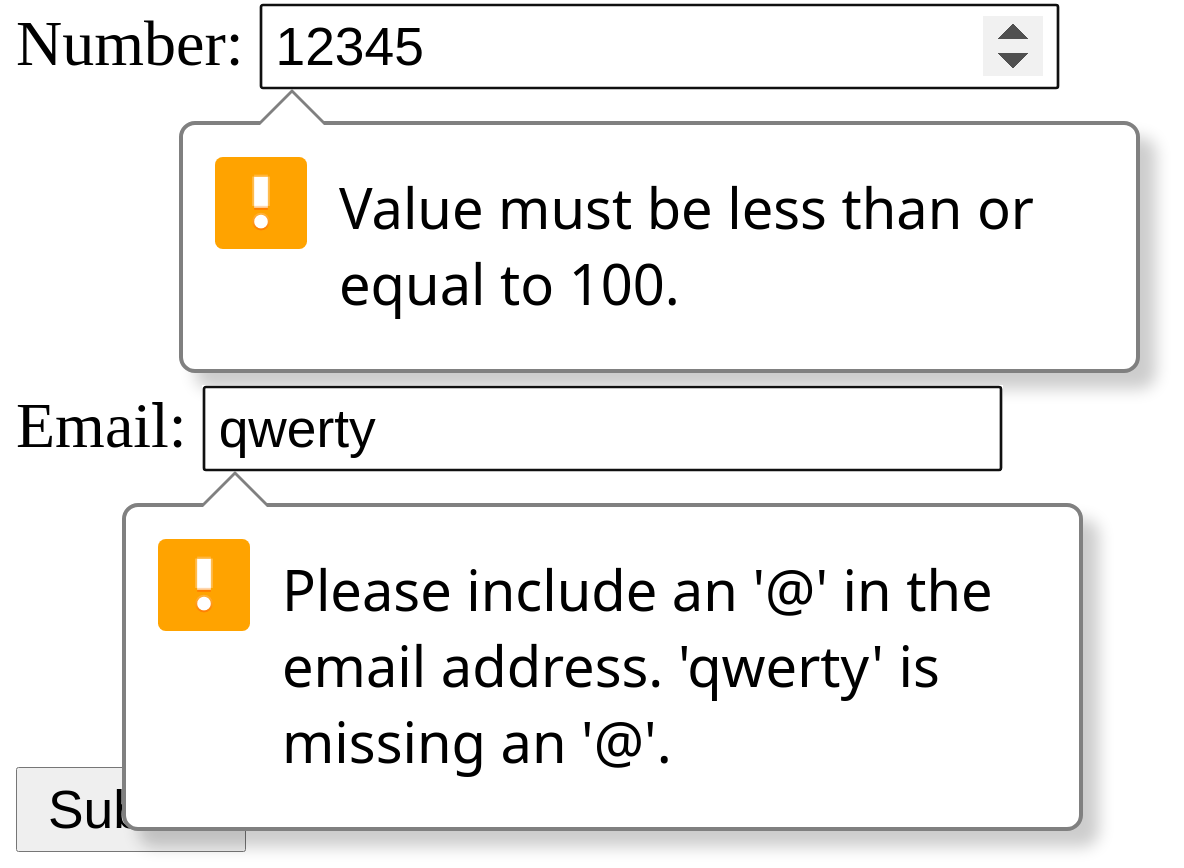
\includegraphics[width=.3\textwidth]{html-form-validation}
    \caption{Error messages that appear after submitting the form on a chromium based browser.}
    \label{fig:html-form-validation}
\end{figure}

Additionally, if the data is sent directly through an \gls{api} call to the backend, Django forms framework ensures invalid data is rejected.
With this, when building a form in Django the developer only needs to specify what fields are present and their type and restrictions and Django will validate all this before data is stored on the database.

Finally, \gls{xss} attacks are prevented because Django escapes the values that were previously provided by users when filling the input tags, e.g. the character ``<'' is transformed in ``\&lt;'', avoiding the browser to interpret user's input as \gls{html} code.

Another problem associated with the views of the MONTRA framework is how the management of javascript dependencies is done.
There is no consistency on how such dependencies are imported.
Some are imported directly on the template through \textit{script} tags making use of a \gls{cdn}, as others their entire source were added to the repository and are then referenced based on their location.
The first approach has the advantage that an upgrade is simply changing the URL attribute of the \textit{script} tag and also reduces bandwidth from the Django server handling the user requests.
The second approach increases the overall size of the repository, and the upgrade process will lead to more changes on the repository.
These processes, however, have the problem that easily unnecessary dependencies will still be present on the Django templates after being used on the application.
Currently, there are tools such as \gls{npm}\footnote{https://www.npmjs.com/} that help to manage these dependencies by defining, on a single file, the dependency and its version.
This software will then download the dependency and subsequent dependencies.

\subsection*{Programming Interface}
% how submissions of fingerprint works

It was mentioned several times that some checks are not enforced through the \gls{api}.
It will be detailed now what calls are performed by MONTRA's fingerprint views.

Note that there are two different \gls{api}s available here.
Fingerprint views use one specific set of \gls{api} requests that return answers in \gls{html} format, ready to present to the user, and others to send the user's data.
For a regular user to use, there are other set o \gls{api} endpoints that are more human friendly, which is documented and has a How to Use page, however, an advanced user can see what requests are made on the fingerprint views through browser's console and perform the requests themselves.

First, we will go over the \gls{api} used by the fingerprint views.
But before showing the available endpoints, let's go over how the fingerprint views are organized and how they show only the questions of a certain question set at a time.

Let use figure \ref{fig:fingerprint-hidden-question-sets} as example.
According to the right side menu, there are six question sets and currently the question set ``Contact Details'' is being presented.
In the middle of the page, we then see the content of the question set: questions, title, control buttons, and permissions.
Note that there is a scroll bar so the question set contains more questions.
Also the previous, next, cancel and save buttons are not tied to the question set.
The other question sets are also present on the page, however, are hidden.
Every question set has its container, so whenever the user clicks on the previous or next buttons or selects another question set on the question set side menu bar, the current question set container is hidden and the new is shown.
For questionnaires with a high number of question sets, rendering all available question sets could not be necessary.
For that, a question set is loaded only when accessed the first time and following accesses will not require a load.

\begin{figure}[H]
    \center
    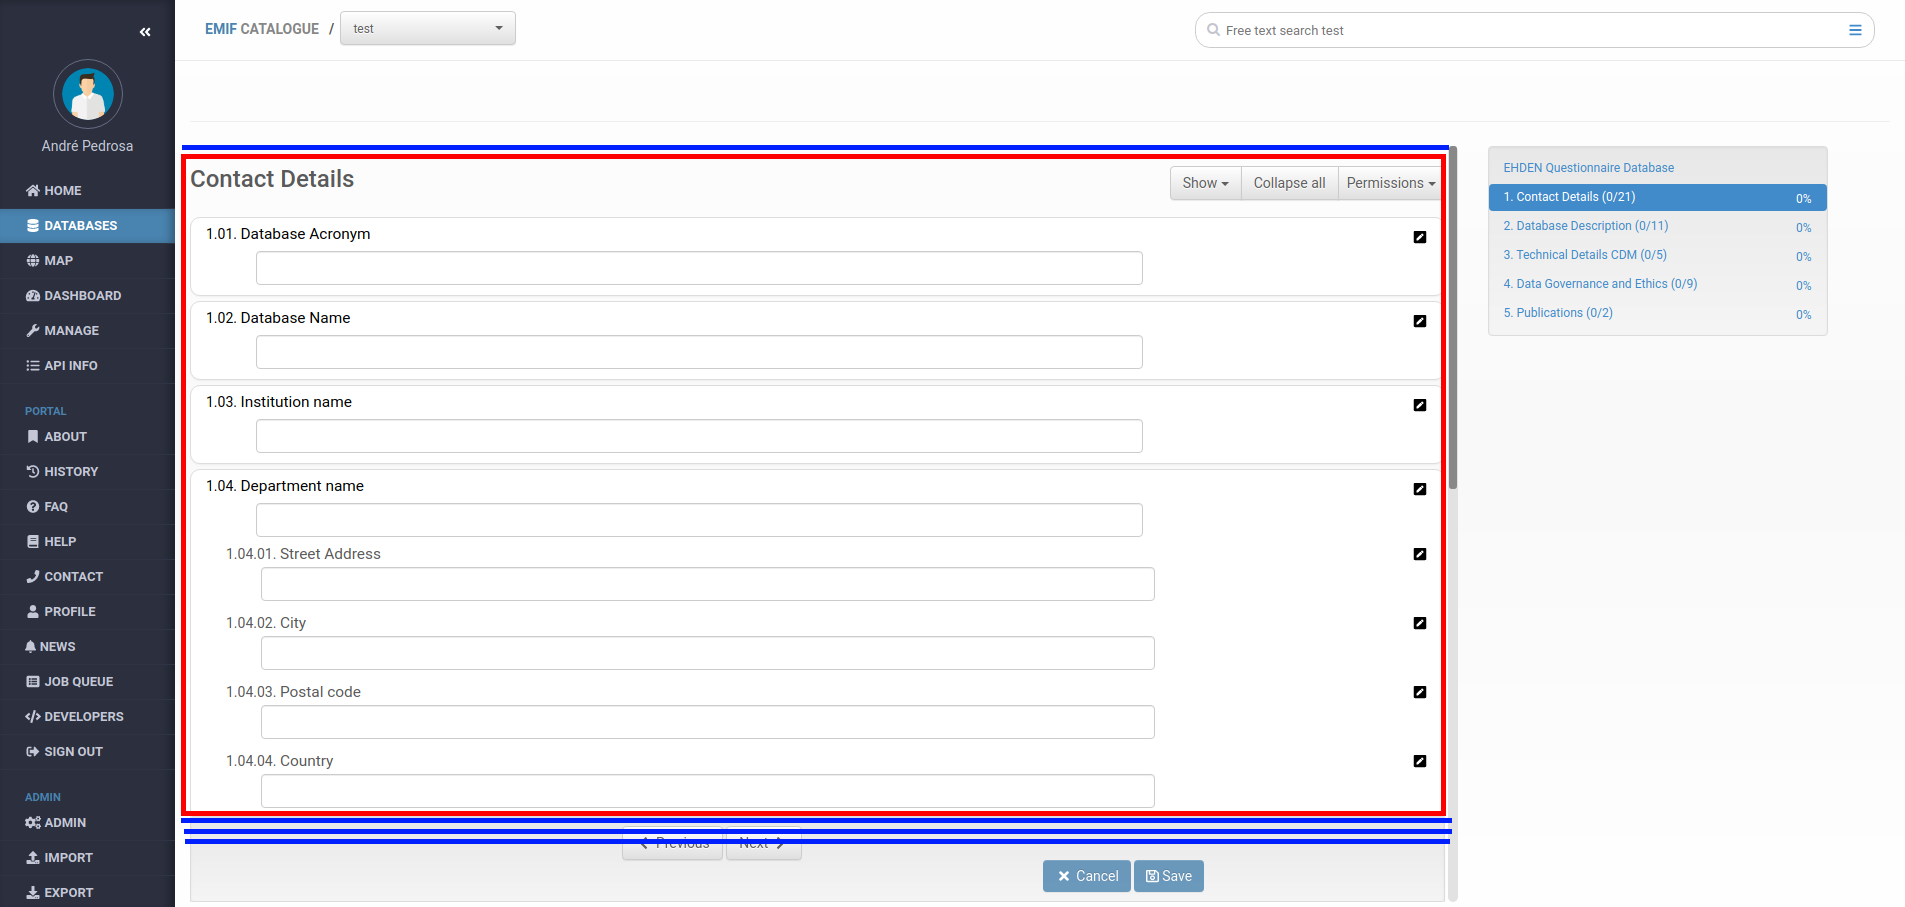
\includegraphics[width=\textwidth]{fingerprint-hidden-question-sets}
    \caption{Each question set has its container.
    Here the current container is presented within the red rectangle.
    The other existing question sets are represented through the blue lines, which currently are hidden.}
    \label{fig:fingerprint-hidden-question-sets}
\end{figure}

The fingerprint view can be used for four different use cases:
\begin{itemize}
    \item Create a new fingerprint: The questions are presented with clear and editable inputs;
    \item Edit an existing fingerprint: All questions are editable but the previously answered questions are filled;
    \item View the answers of a fingerprint: A read-only version of the fingerprint's answers;
    \item Search for fingerprints: Same as creating a new fingerprint, however, no validations are performed on the user's input.
\end{itemize}

For these use cases, the following endpoints are used:

\begin{itemize}
    \item Create:
\begin{lstlisting}[basicstyle=\tiny]
GET [base url]/c/[community slug]/addqs/[fingerprint hash]/[questionnaire id]/[question set id]/
POST [base url]/c/[community slug]/addPost/[questionnaire id]/[question set id]/[save id]
\end{lstlisting}
    \item Edit:
\begin{lstlisting}[basicstyle=\tiny]
GET [base url]/editqs/[fingerprint hash]/[questionnaire id]/[question set]/
POST [base url]/c/[community slug]/addPost/[questionnaire id]/[question set id]/[save id]
\end{lstlisting}
    \item View:
\begin{lstlisting}[basicstyle=\tiny]
GET [base url]/detailedqs/[fingerprint hash]/[questionnaire id]/[question set id]/
\end{lstlisting}
    \item Search:
\begin{lstlisting}[basicstyle=\tiny]
GET [base url]/c/[community slug]/searchqs/[questionnaire id]/[question set id]/
\end{lstlisting}
\end{itemize}

For both cases where new data is stored, besides the usual GET that is used to load the question set, there is also a POST request that saves the progress done to a specific question set.
The data for these requests are gathered natively by javascript once each question set container contains a \textit{form} tag englobing all the questions inputs.
This way there is no need to iterate over the questions of a question set and append each response to the request's data.
The \textit{save id} field of the endpoints tells to which question set the data is related to
However, there is already a \textit{question set} field which always has the value of 1, so one of these fields could be removed from the endpoint.

The GET request is then used to load the \gls{html} to present the questions of a question set.
Note that the returned data is just the \gls{html} data to be placed on the respective question set container and not the whole fingerprint page.

Moving now to the set of \gls{api} endpoints available to the users to both read and update answer data the following are available:

\begin{verbatim}
GET /api/fingerprints/[fingerprint hash]/answers/
GET /api/fingerprints/[fingerprint hash]/answers/[question slug]
PUT /api/fingerprints/[fingerprint hash]/answers/[question slug]
\end{verbatim}

The first two GETs are used to retrieve answers data, which is returned as the \gls{json} object presented next, the only difference being the first one returns an array of the mentioned object instead of just one.

\begin{verbatim}
{
  "question":"patients_count",
  "data":""
}
\end{verbatim}

With the PUT request, a fingerprint owner can update data of specific answers where a \gls{json} object should be sent in the body of the request with the field ``data''.

\begin{verbatim}
{
  "data": 10000
}
\end{verbatim}

Existing two different types of endpoints to retrieve answers data makes sense since the returned format is returned in a way that is easier to handle data by the target entity that will consume that endpoint.
If the fingerprint pages receive the data in \gls{html} format they can just put the \gls{html} in the determined container instead of having to build the entire container and insert the data on each input.
Accordingly, if data is returned in a \gls{json} format it can easily access the data and perform some data processing avoiding going transverse the \gls{html} and retrieve the data from each input.
However, having two different endpoints to update data does not make that much sense since current \gls{http} requests libraries offer an easy way to build a request in the required format as the one's browsers automatically build whenever a form is submitted.

\subsection*{Draft Status Changes}

We will also go over the \gls{api} endpoints that the front end code uses to request to change the fingerprint state from draft to published.
Associated with this feature, there are two endpoints available:

\begin{verbatim}
POST [base url]/api/pending/[fingerprint hash]
POST [base url]/api/draft/[fingerprint hash]
\end{verbatim}

The existence of two endpoints for the same purpose is because Communities have a setting that allows to auto-accept requests to publish a fingerprint.
For that, whenever the auto-accept setting is off, the first endpoint must be used, which will send a request to the community owners to publish the given fingerprint.
The second must be used otherwise.

The problem with this approach is that the code that decides what endpoint to use is on the client-side and there is no server-side check if the correct endpoint is being used.
If the auto-accept setting is off and the second endpoint is used, a user can publish his fingerprint without requiring the approval of the community owners.

\subsection{Import Questionnaires - Excel}
\label{subsection:excel}
% Como os vários conceitos anteriores são mapeados para o excel
% Question Sets
% Questions
% Choices
% ...

As mentioned before, to define a skeleton of the metadata that describes a data source for a given community, a spreadsheet file has to be submitted.
There is already a template with some instructions and columns where a community manager only has to fill the necessary rows to then get the wanted result.

The column defined in the template are the following:
\begin{itemize}
    \item Type: the type of the specific row. Here are allows 3 different values:
        \begin{itemize}
            \item QuestionSet: allows dividing the questionnaire into several sections;
            \item Question: a question specification;
            \item Category: allows to create a group of questions inside a question set.
        \end{itemize}
    \item Text/Question: label/name given to the item being defined;
    \item Level/Number: use as a level for questions and categories and number otherwise. As level allows to create groups of questions inside a question set. As number defines the number, and subsequently the order, of the question sets;
    \item Data type: used only for rows of type Question, specifying the question type;
    \item Value list: used to indicate extra information to build the question;
    \item Help text/Description: a small text that will be displayed along with the item being defined;
    \item Tooltip: Yes if the Help text/Description should be displayed as a tooltip or No otherwise;
    \item Slug: internal identifier;
    \item Dependencies: used to tell that a question or group of questions can only be answered if a specific choice of a choice-based question was selected;
    \item Stats, Comments Stats and Disposition: Columns that were used for old features but are still present on the spreadsheet;
    \item Include in Advanced Search: if the answers of the question can be used to search fingerprints.
\end{itemize}

\subsection*{Question Groups}
From the previous list, question groups were mentioned both when the type column has the Category value and on the Level part of the Level/Number column.
The former is used to add a title with no question associated, resulting in what is presented in figure \ref{fig:question-group-category}.

\begin{figure}[H]
    \center
    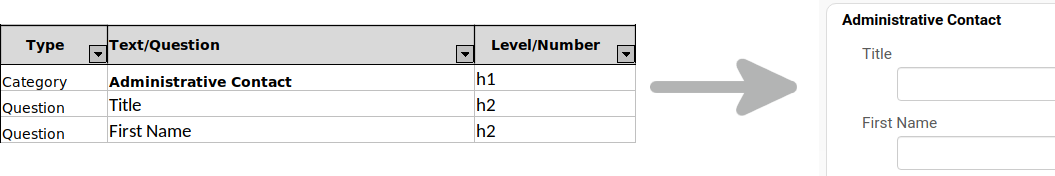
\includegraphics[width=\textwidth]{category}
    \caption{Create a group of questions with a title.}
    \label{fig:question-group-category}
\end{figure}

On the latter, the text of the question in the most upper level is used as the title of the questions group, resulting in an output similar to the one in figure \ref{fig:question-group-levels}.

\begin{figure}[H]
    \center
    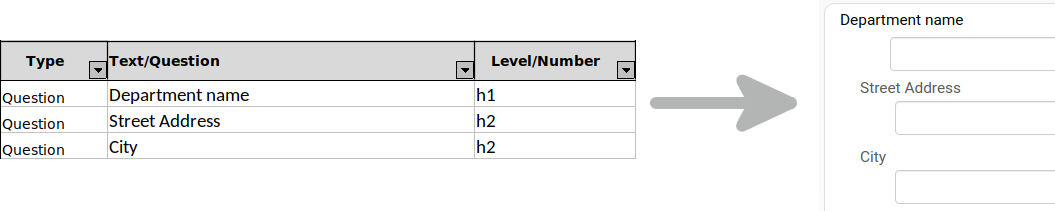
\includegraphics[width=\textwidth]{levels}
    \caption{Create a group of questions using a question's text as the title.}
    \label{fig:question-group-levels}
\end{figure}

It is important to highlight that the category way to create question groups is not independent of levels.
If both a category row and a question are on the most upper level, MONTRA will render two separate collapsable containers, where the first one will be empty, as is shown in figure \ref{fig:question-group-category-wrong-levels}.

\begin{figure}[H]
    \center
    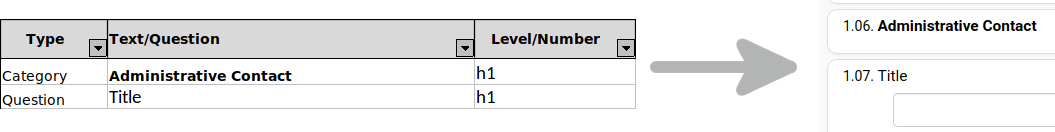
\includegraphics[width=\textwidth]{category-levels}
    \caption{Example to show that the category way to create question groups also depends on the values that are set on the level column.}
    \label{fig:question-group-category-wrong-levels}
\end{figure}

\subsection*{Value list}

To avoid having a spreadsheet with several columns that will not be used for all types of rows, the value list column expects some extra information required for some types of questions.

\subsubsection*{Choices}

For choice-based questions, the value list column is used to define the possible choices and to add an extra text field associated with a given choice.
Choices are separated by a ``|'' character and the extra text field can be set by appending ``\{...\}'' after the target choice's text.

\begin{figure}[H]
    \center
    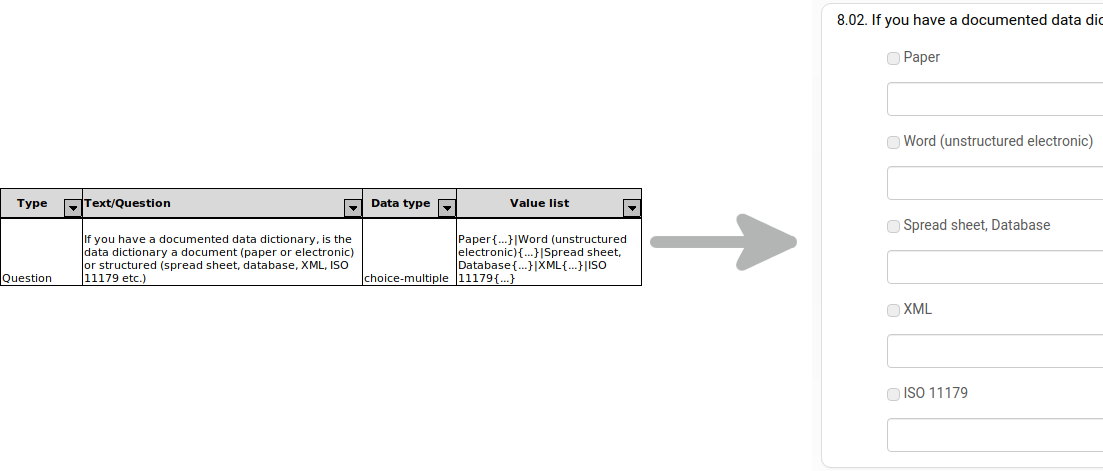
\includegraphics[width=\textwidth]{choice-freeforms}
    \caption{Multiple choice question with some extra text fields associated with the several choices.}
\end{figure}

Although the framework allows the extensibility to have an additional text field, these do not support other types of input and also have no validation.
Also, if the number of choices is high and the text is long, there starts to exist some clutter on the spreadsheet.
With this, the person creating the spreadsheet will have problems perform edits and check if there is something wrong or missing.

To facilitate the job of who is filling the spreadsheet, some question types are shortcuts.
For example, the choice-yesnodontknow is a question of type choice with three possible options: Yes, No, Do not Know.
Choice variants with freeform on the name, besides the usual choices, always have an additional text field, associated with the question instead of a choice.

\subsubsection*{Open Multiple Composition}

Open multiple questions allow showing a history of a given value.
For that the simple version of the question is represented in a table of two columns: Date and the value, so no input is expected on the value list column.
The composition version of the question type allows having several values, instead of just one.
In a way, the simpler version can be used as a shortcut question type, since it can be reproduced with the composition variant.

To render this question type, a third-party widget called Tabulator\footnote{http://tabulator.info/} is being used.
The configuration of such widget, expects an array of \gls{json} objects, each specifying some configuration of each column.
To configure the open multiple composition question type, the value list column expects these \gls{json} objects, where the date column is implicit.
The MONTRA framework will then put the provided objects on the configuration array that the Tabulator widgets expects, adding the configuration for the date column.

\begin{figure}[H]
    \center
    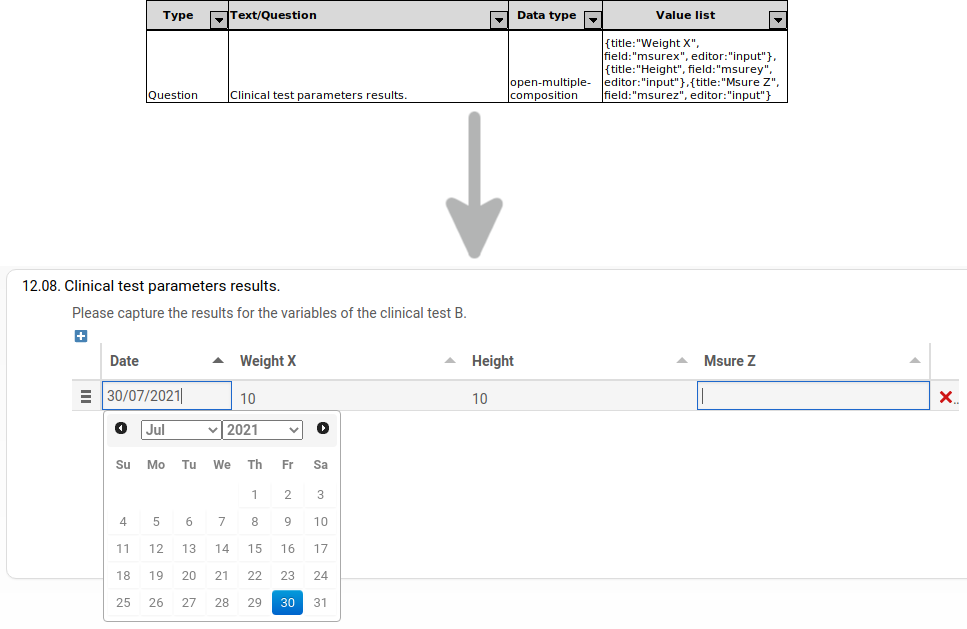
\includegraphics[width=\textwidth]{open-multiple}
    \caption{How an open-multiple-composition question type is specified on the spreadsheet and how it is rendered.}
    \label{fig:open-multiple}
\end{figure}

\subsubsection*{Choice Tabular}

This type of question allows reusing the same choices across several answering items.
There are three variations of this questions types, where the difference between them is what and how is the information connected between answering items and choices.
There are two versions where the user can select one (single choice) or more (multiple-choice) choices for each answering item.
The other version allows the user to write text for each choice within each answering item.
The question type is rendered as a table where in the columns are displayed the several choices and on the rows the different answering items are presented.
Additionally, there can be a ``More'' choice column, where the user can insert any text information for a specific answering item since is displayed with a textarea \gls{html} element.

The value list column of a choice tabular question type expects a three-component value.
Each component is separated by the characters ``\textbackslash\textbackslash''.
Within each component, items are separated by the ``|'' character.
The components are the following:

\begin{itemize}
    \item choices (columns);
    \item answering items (rows);
    \item type of the information: available values are choice, multiple-choice and text.
\end{itemize}

Once again, we encounter the clutter problem, as shown in the spreadsheet section of figure \ref{fig:choice-tabular}, which hampers readability and update of the value list field.

\begin{figure}[H]
    \center
    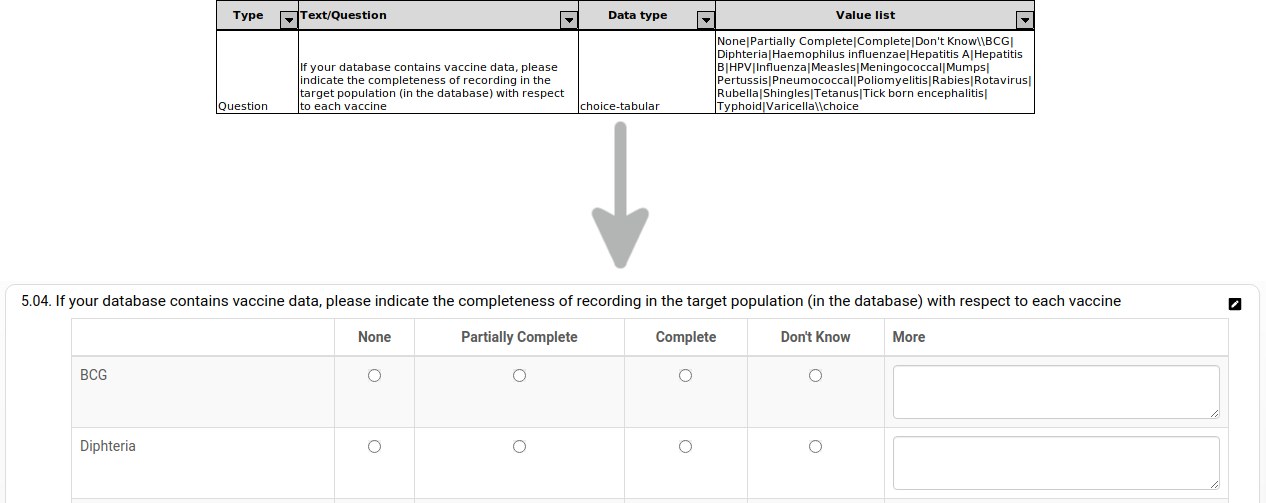
\includegraphics[width=\textwidth]{choice-tabular}
    \caption{How a tabular-choice question type is specified on the spreadsheet and how it is rendered.}
    \label{fig:choice-tabular}
\end{figure}

\subsection*{Dependencies}

In several form applications, it is common to find situations where if a certain choice is selected, then other questions will show up.
E.g. If a user answers ``Yes'' to the Question ``Have you visited Aveiro?'', then other questions such as ``Would you recommend it to a friend?'' would appear.

MONTRA supports this kind of dependencies, which should be defined on the Dependencies column of the questionnaire spreadsheet.

\begin{figure}[H]
    \center
    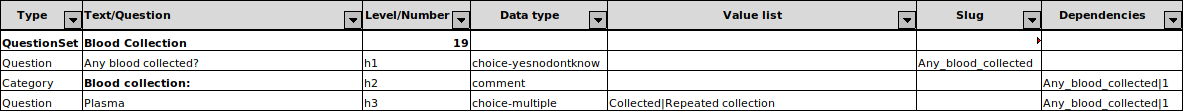
\includegraphics[width=\linewidth]{dependencies-excel}
    \caption{An example of both a question and a category that depend on the selected value for another question.}
    \label{fig:dependencies-excel}
\end{figure}

As shown in figure \ref{fig:dependencies-excel}, first you should indicate the slug of the question on which the specific question depends.
Then, separated by a ``|'' character, it must be specified which choice has to be selected for the dependency to be fulfilled, using its index, starting at 1.
On figure \ref{fig:dependencies-excel}, since a choice-yesnodontknow question type has three implicit choices, by having a dependency with the value ``Any\_blood\_collected|1'', both the \textit{Blood collection} category and the \textit{Plasma} question will only be displayed to the user once the choice \textit{Yes} of the \textit{Any Blood Collection?} question is selected.

\begin{figure}[H]
    \center
    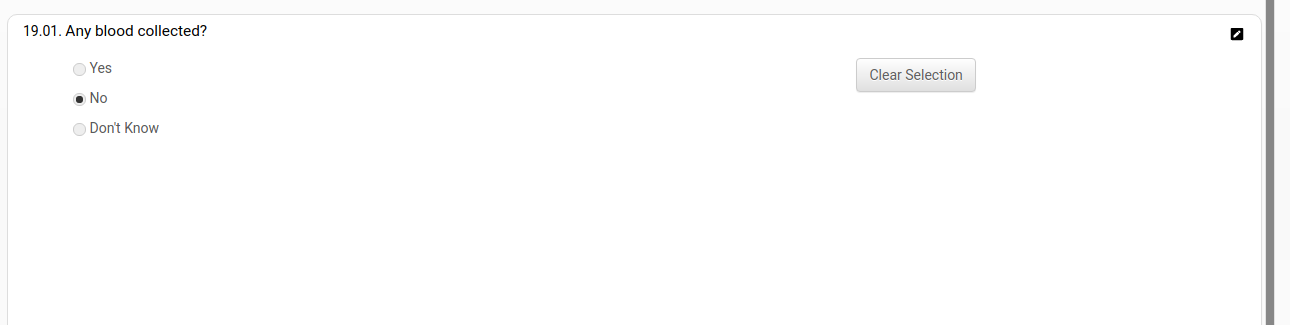
\includegraphics[width=0.75\linewidth]{dependencies-no}
    \caption{The questions with dependencies are not rendered if the specific choice is not selected.}
    \label{fig:dependencies-no}
\end{figure}

\begin{figure}[H]
    \center
    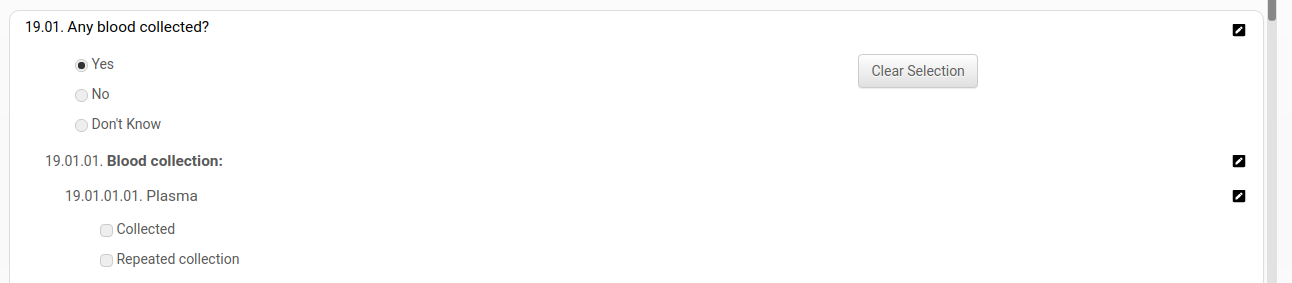
\includegraphics[width=0.75\linewidth]{dependencies-yes}
    \caption{Once the dependency of a specific question is meet it will be rendered.}
    \label{fig:dependencies-yes}
\end{figure}

Besides such restrictions are imposed on the user when he visits the web page, if the API was used directly, such dependencies would not be checked, which would lead to unnecessary data be stored on the database since it will not be displayed to the user.

\subsection{Data Models}
% Diagrama de classes
% Principal intuito de cada class
% answers (todos os tipos guardados em texto)

This section will present how the previous concepts are mapped to database models.
Taking advantage of Django's \gls{orm} feature, MONTRA's data models are defined as python classes that extend Django's base Model class.
These Model classes belong to different applications, which are associated with distinct aspects of the platform.

In figure \ref{fig:old-models} is presented the class diagram of the classes that are related to features and/or concepts that were mentioned in previous sections.
Classes with the same color belong to the same Django application, dividing them into specific purposes.

\begin{figure}[H]
    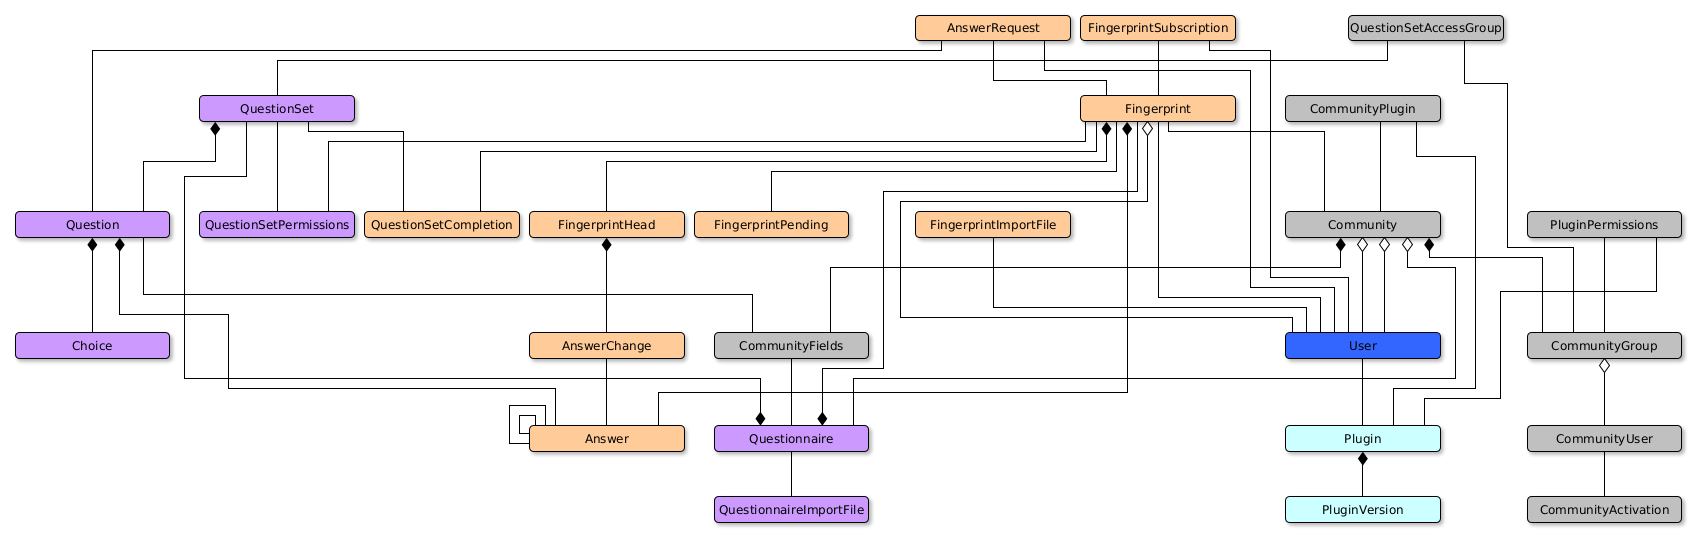
\includegraphics[width=\textwidth]{old-models}
    \caption{Class diagram of MONTRA's Model classes. Each color has a Django application associated. Gray: Community; Purple: Questionnaire; Orange: Fingerprint; Light Blue: Plugin; Blue: Django Auth. MONTRA's data model is much more complex, however, it is just presented the ones that impact the features and/or concepts mentioned previously.}
    \label{fig:old-models}
\end{figure}

\begin{itemize}
    \item Blue - Django's built-in authentication system\footnote{https://docs.djangoproject.com/en/1.11/ref/contrib/auth/};
    \item Orange - Fingerprint application: Answers to questionnaires questions and other models associated with features that were mentioned on the fingerprint views section, such as AnswerRequest and FingerprintSubscription.
        MONTRA also keeps a record of all the states of a given Fingerprint.
        For that, it uses the FingerprintHead model, which maps to a set of AnswerChanges;
    \item Purple - Questionnaire application: Questionnaires structure information such as question sets, questions, and choices, and import spreadsheets logs. Additionally, associated with each fingerprint, contains a model with the allowed permissions on each question set;
    \item Light Blue - Developer application: Allows adding customizations to different MONTRA's installations through plugins;
    \item Gray - Community application: Community's groups, users and access permissions, fields to be presented on the fingerprint list page for each questionnaire and plugins.
\end{itemize}

% ---

Going into more detail on some models we can see some poor design decisions.

Regarding fingerprint answers to a questionnaire, all the data is stored in the Answer model on the data field, which is a variable-length string field type.

\begin{figure}[H]
    \center
    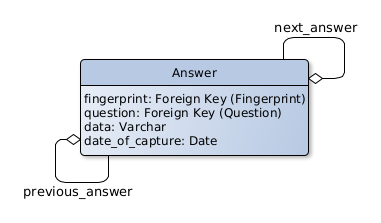
\includegraphics[width=.4\linewidth]{answer-model}
    \caption{Detailed information of the Answer model of the Fingerprint application.}
    \label{fig:answer-model}
\end{figure}

Although this approach is much simpler in terms of data models, it leads to two problems:
\begin{enumerate}
    \item this is not the most optimized way to store all the data types.
        Some question types expect numeric values and other date values, which could use built-in field types of a \gls{rdbms};
    \item for complex question types which the answer contains several fields, before and after storing such data in the database, some processing has to be made to convert the data to the necessary format.
        One example of this is multiple choice questions, where the value of the several selected choice is joined in a single string to then be stored on the database.
        Every time the answer needs to be displayed to a user, it is necessary to split that string by its separator.
        For this situation instead of storing the choice's value, the models of the questionnaire application could be used as a foreign key.
\end{enumerate}

Related to MONTRA itself, when a user provides no data to a specific question, an empty string will still be sent for that question on the submission of the answers to a question set, which will create unnecessary records on the database.

As mentioned previously, MONTRA records the history of submissions for a specific fingerprint.
Each submission has an associated FingerprintHead record, which its name might have been inspired by the HEAD concept of Git\footnote{https://git-scm.com/}, a version control system.
For every FingerprintHead there is a set of answers that suffer changes which are then recorded on the AnswerChange model.
In this model, we can get the answers data duplicated three times since it is already stored on the Answer model and can also be stored again as text in both \textit{old\_value} and \textit{new\_value}.

\begin{figure}[H]
    \center
    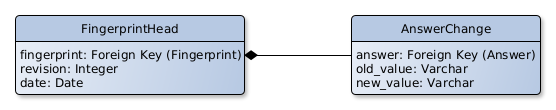
\includegraphics[width=.6\linewidth]{answer-changes-models}
    \caption{Models that store the changes to answers of fingerprint.}
    \label{fig:answer-changes-models}
\end{figure}

% ---

As mentioned previously, a fingerprint is not immediately available to all regular users, since it first enters on a draft state.
To transit to the published state, a request needs to be made to the community owner.
Such requests are stored on the FingerprintPending table, where the pending value will be \textit{true}.
Once a request is rejected or accepted, the value of the pending value is changed to \textit{false}.

\begin{figure}[H]
    \center
    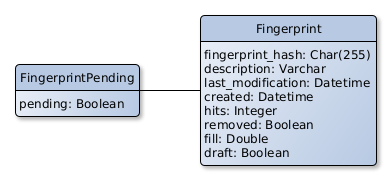
\includegraphics[width=.6\linewidth]{fingerprint-pending-models}
    \caption{The Model that stores the information telling if a fingerprint is waiting to be approved to be published.}
    \label{fig:fingerprint-pending-model}
\end{figure}

On the Fingerprint model, there is also a \textit{draft} value that indicates if the fingerprint is published or not.
Once a fingerprint is published, the value of the \textit{draft} will be true, and on the FingerprintPending table, the associated record will have the pending value at \textit{false}.
However, this value is not required to be stored on the database since after a fingerprint is published, the fingerprint will not be pending therefore, the associated FingerprintPending record could be deleted.

% ---

Whenever a questionnaire is imported, a QuestionnaireImportFile record is created containing the information of the uploaded file and the user that uploaded it.
Also contains a status field to give some feedback to the user.
Associated with every import will also be created a Questionnaire record.
It contains an in\_preview variable that is set to \textit{true} whenever a questionnaire is in the import process.
If it fails to import, only the QuestionnaireImportFile record will be kept, which the status will change to \textit{Failed} and an error message will also be attached to the import record.

\begin{figure}[H]
    \center
    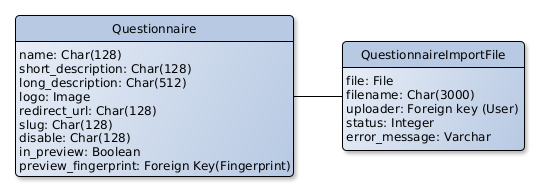
\includegraphics[width=.6\textwidth]{questionnaire-import-models}
    \caption{Questionnaire model and the model where questionnaire imports information is stored.}
    \label{fig:questionnaire-import-models}
\end{figure}

If the questionnaire is valid, the user will be redirected to a page where he can preview the result and can accept or reject it.
It is important to point out that for the preview process a new Fingerprint object is created so \gls{api} calls can be performed.

Strangely on the Questionnaire model, the disable column uses a character type column instead of a boolean one since it expects only the value of ``False'' and ``True''.
If there are some user input errors, it could lead to unexpected behavior or internal server error.

% ---

Associated with how the structure of a questionnaire is stored, there are only four models to do so: Questionnaire, QuestionSet, Question, and Choice.
All are associated with a specific concept of the questionnaire, although other concepts are not represented.
First, there's the category, used to create question groups within a question set.
It is represented as with a question record, where the ``category'' field of the question models has the value ``true''.
For more complex question types, that require extra configuration, such as choice tabular (name of the rows and column) and open multiple (name of the columns), such data is stored in a metadata field of the associated question model.
Question types that do not make use of these fields, will have an empty value, leading to some database space being wasted.

\begin{figure}[H]
    \center
    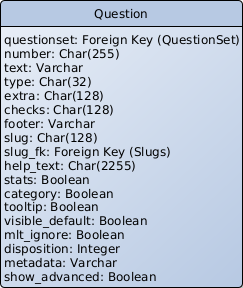
\includegraphics[width=.3\textwidth]{question-model}
    \caption{Question model and its extensive number of fields.}
    \label{fig:question-model}
\end{figure}

When the questionnaire's spreadsheet was explained, some fields were related to some old deprecated features.
The question model contains the same fields that map to the questionnaire's spreadsheet deprecated fields: stats, visible\_default, and disposition.
There is also a slug\_fk field that points to a Slugs model that replicates the question's slug and text, which is was used to yet another deprecated feature.

Finally, a question supports for the user to define additional checks which are defined on the ``checks'' field however, this feature is not exposed through the questionnaire's spreadsheet.

\section{Refactoring}
% o que necessita de, ou vai, ser alterado

Until now it was shown how the MONTRA framework was designed around databases, their metadata, and how that metadata can be shared among the platform users.
For regular users the framework provides a good user experience, however, for power users, that make use of \gls{api}s, might make some errors which the framework will not prevent, leading to inaccurate data to be stored and presented.
Also for developers, such flaws and bad design choices make the maintainability process of MONTRA instance a demanding and tedious process.

With this, there is a clear opportunity to perform a refactoring process over the framework to correct such problems and the issues that have been emphasized in this chapter.
The goal of this refactoring process is not to change the framework in a way to transform existing use cases, but to improve its internal structure to make the framework more stable, easier to maintain, and easier for an external tool to communicate with it, mainly to publish database data.

Next, we will propose several changes to be applied to the framework, beginning from the data models, regarding how fingerprint answers data is stored, how questionnaires structure is stored and some other fixes for some defects explained previously.
Such refactoring will imply changes on other components, one of them being the rendering of questionnaires and how input validation is done.
Finally, several clutter problems were mentioned when describing the spreadsheet to define a questionnaire structure, so the spreadsheet will also undergo a refactor.

\subsection{Data Models}
% explicar escolha de apenas reformular apenas a apartir de determinado nivel
% explicar os novos modelos e de que maneiras resolvem problemas que existiam
% trade offs tidos em conta
% diagrama de classes com diferenças

Since the MONTRA framework uses some outdated software and there are active installations, the refactoring process can not be simply designing new models and views, implementing them, and replacing old ones is not a viable option.
The approach taken was to first decide what components would go through a refactoring process and within each, until what level we would apply it.

Taking into account figure \ref{fig:old-models}, since both the Community and Developer (Plugins) Django applications target functionalities not so fingerprint-centric and are more related to features of the framework as a whole, we decided not to perform any changes on the models of these applications.
This leaves us with both the Fingerprint and Questionnaire applications.
Regarding the Fingerprint application, the fingerprint model is one of the main models of the framework, affecting several features of the framework, so we intend to perform minimal changes on it.
However, the remaining models associated with the answers of a fingerprint and submissions will have a new models design.
Respecting the Questionnaire application both the Questionnaire and QuestionSet models represent well-defined concepts and do not require any changes.
Yet, the remaining models, mainly the models storing the structure of the questions, their dependencies, choices, etc.\, will also have a new design.

In Figure \ref{fig:new-models} it is presented the new models in light green.
The decided approach to implement these models was to create a new Django application and create all these new models on that application.
This way, the migration process is an iterative process where the framework is always operational since the previous models still exist.
Then with the help of an \gls{ide}, we can search for usages of the old models and migrate each feature at the time.

\begin{figure}[H]
    \center
    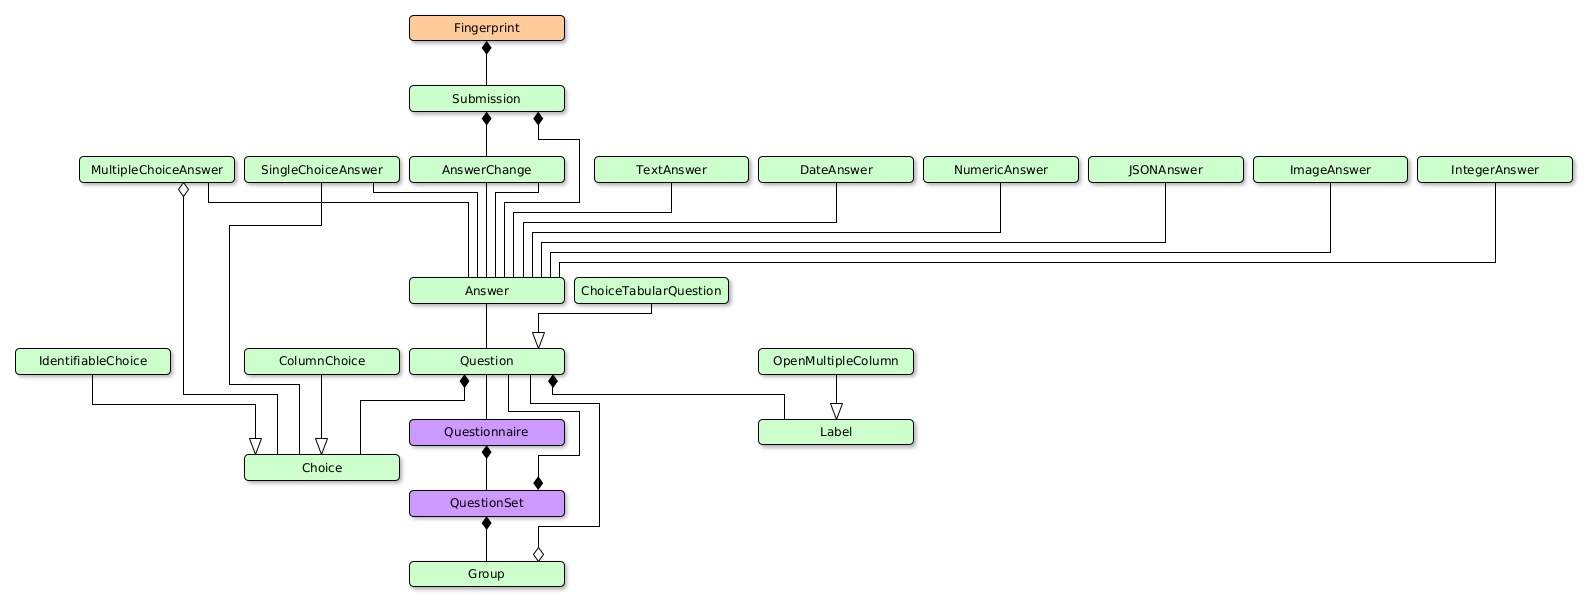
\includegraphics[width=\textwidth]{new-models}
    \caption{Model Diagram of the new models.}
    \label{fig:new-models}
\end{figure}

Let's start with the fingerprint-related changes.
Now there is a new Answer model that does not hold directly the content of answers, instead the content is stored on data-specific models such as IntegerAnswer and DateAnswer.
For choice-based questions, instead of storing the value of the selected choice(s), a single or multiple choice answer contains a foreign key(s) for the selected choices.
To establish the connection between the main Answer model and the data-specific model, the main model contains a \textit{type} field that indicates the data type of the answer.
Then the primary keys of the data-specific answer model are the same as the associated record of the Answer model, which allows fetching the data-specific answers of an Answer.
Is important to note that the number of different answer types is not the same as the number of question types.
Answers of different questions types can be stored in the same answer type models, for example, open text and email questions both can be stored as text in the database.
Previously fingerprint submissions were being represented with the model FingerprintHead, now we created a Submission model which contains the same relationships as before, a set of answers, a set of answer changes, all this associated with a fingerprint.
The AnswerChange model now does not contain the data of the previous and current answers, instead, it contains the foreign keys for the answer model.
In cases where the change was from or to an empty answer, either the previous answer or the next answer field are filled with the NULL value.

Moving now to the models related to the Questionnaire application, there is a new Question model mainly because the previous one had too many fields.
An example of these extra fields is the \textit{metadata}, which is used to store the information of the column of the open-multiple question type and the choices and answering items of a choice tabular question type.
This field was replaced by the addition of new models (Label) which will be explained in more detail in the next Excel subsection.
Another example was the category field, which indicated if a specific question record described a category in the questionnaire which was being used to create subgroups of questions.
With the new models, a new Group model was created which has a set of questions associated.
Previously this relationship did not exist, so MONTRA would create a group based only on the question's order and level.
Additionally, with the addition of this Group model, there is no need to have a level field on the question type, since nested levels are represented through Groups, which can have a parent group.
A group with no parent is represented in the root level of the questionnaire.
The remaining models (Label, Choice, and their descendants) will be explained in more depth in the next Excel subsection since they were created mainly because of how questions are represented in the new spreadsheet format.

Meanwhile, there are previously existing models that have undergone changes to fix some design flaws mentioned before.

\begin{itemize}
    \item QuestionnaireImportFile: To provide feedback to the user this model only contained an \textit{error\_message} field.
        However several times there are some errors with the questionnaire, but the framework can continue.
        In these situations, a warning could be sent to the user just so he is aware that a part of the spreadsheet has some errors and the result could not be his real end goal.
        Then the new model contains two new fields, \textit{errors}, replacing the old \textit{error\_message}, and \textit{warnings} fields, which are stored in \gls{json}, where the keys are the lines where the errors or warnings were found and the values are an array of messages associated with that line;
    \item Questionnaire: associated with the questionnaire model we mentioned that it had a specific fingerprint attached that was used to show a preview of the result of the questionnaire.
        This field is not required since the preview mode of a questionnaire is viewed on read-only, so no answers are associated with these preview fingerprints;
    \item QuestionSetPermissions: From this model, we removed the useless permission of ``Allow Printing'', considering it is impossible to restrict users from printing the page since a screen capture software can be used as a replacement for the browser's print function.
        Also, there was a record associated with each question set of every fingerprint, even if the values of each permission were the default ones.
        The new approach taken is to only create a record if any permission value is different from the default one.
        Otherwise, an object with the default values is returned;
    \item Fingerprint: It has a new ``submission\_token'' used for the new \gls{api} endpoints explained next.
\end{itemize}

\subsection{Views}

When the MONTRA framework was presented it was highlighted that the different variations of the fingerprint view (create, show, edit, search, preview) were all using a different Django template.
Once again, this brings the problem that one change will entail that the same change has to be applied on the remaining fingerprint view variations.
On the refactoring process, these views were adapted so all the different pages use a shared fingerprint template which then renders the necessary components according to the page where are being rendered.

The first step of this process is to put different components into separate templates, which will then allow the creation of different arrangements of such components according to the fingerprint view variation being displayed.
Note that even within these new separate components, some parts of them might be rendered differently according to the fingerprint view variation where they are being inserted into.
In figures \ref{fig:fingerprint-new} and \ref{fig:fingerprint-show-detailed} we can see that some components are present on both views.
The question set title, the questions, the question set menu, the fill progress bar, and the navigation buttons.
However, we can also see some components in figure \ref{fig:fingerprint-show-detailed} which are not present on the on figure \ref{fig:fingerprint-new} such as the fingerprint statistics (hits, unique views and fill percentage), there are no fingerprint-related buttons, which are now questionnaire-wide buttons.
Note that the name of the fingerprint (DemoAveiro), the several tabs (Fingerprint, Documents, etc.) and the subscribe and Manage buttons are specific to the show Page.
The new fingerprint template will only contain components to display within the Fingerprint tab.

In Figure \ref{fig:fingerprint-other-after-diagram} is presented a two-column layout for the create, edit, search and preview variations of the fingerprint view.
Although, some components are not displayed in certain variations, such as the Cancel and Save buttons.
The Cancel button is not displayed on the preview variation, and both Cancel and Save buttons are replaced by a Search button on the search button.
Additionally, different buttons appear on the question set buttons component according to the fingerprint view variation.

\begin{figure}[H]
    \center
    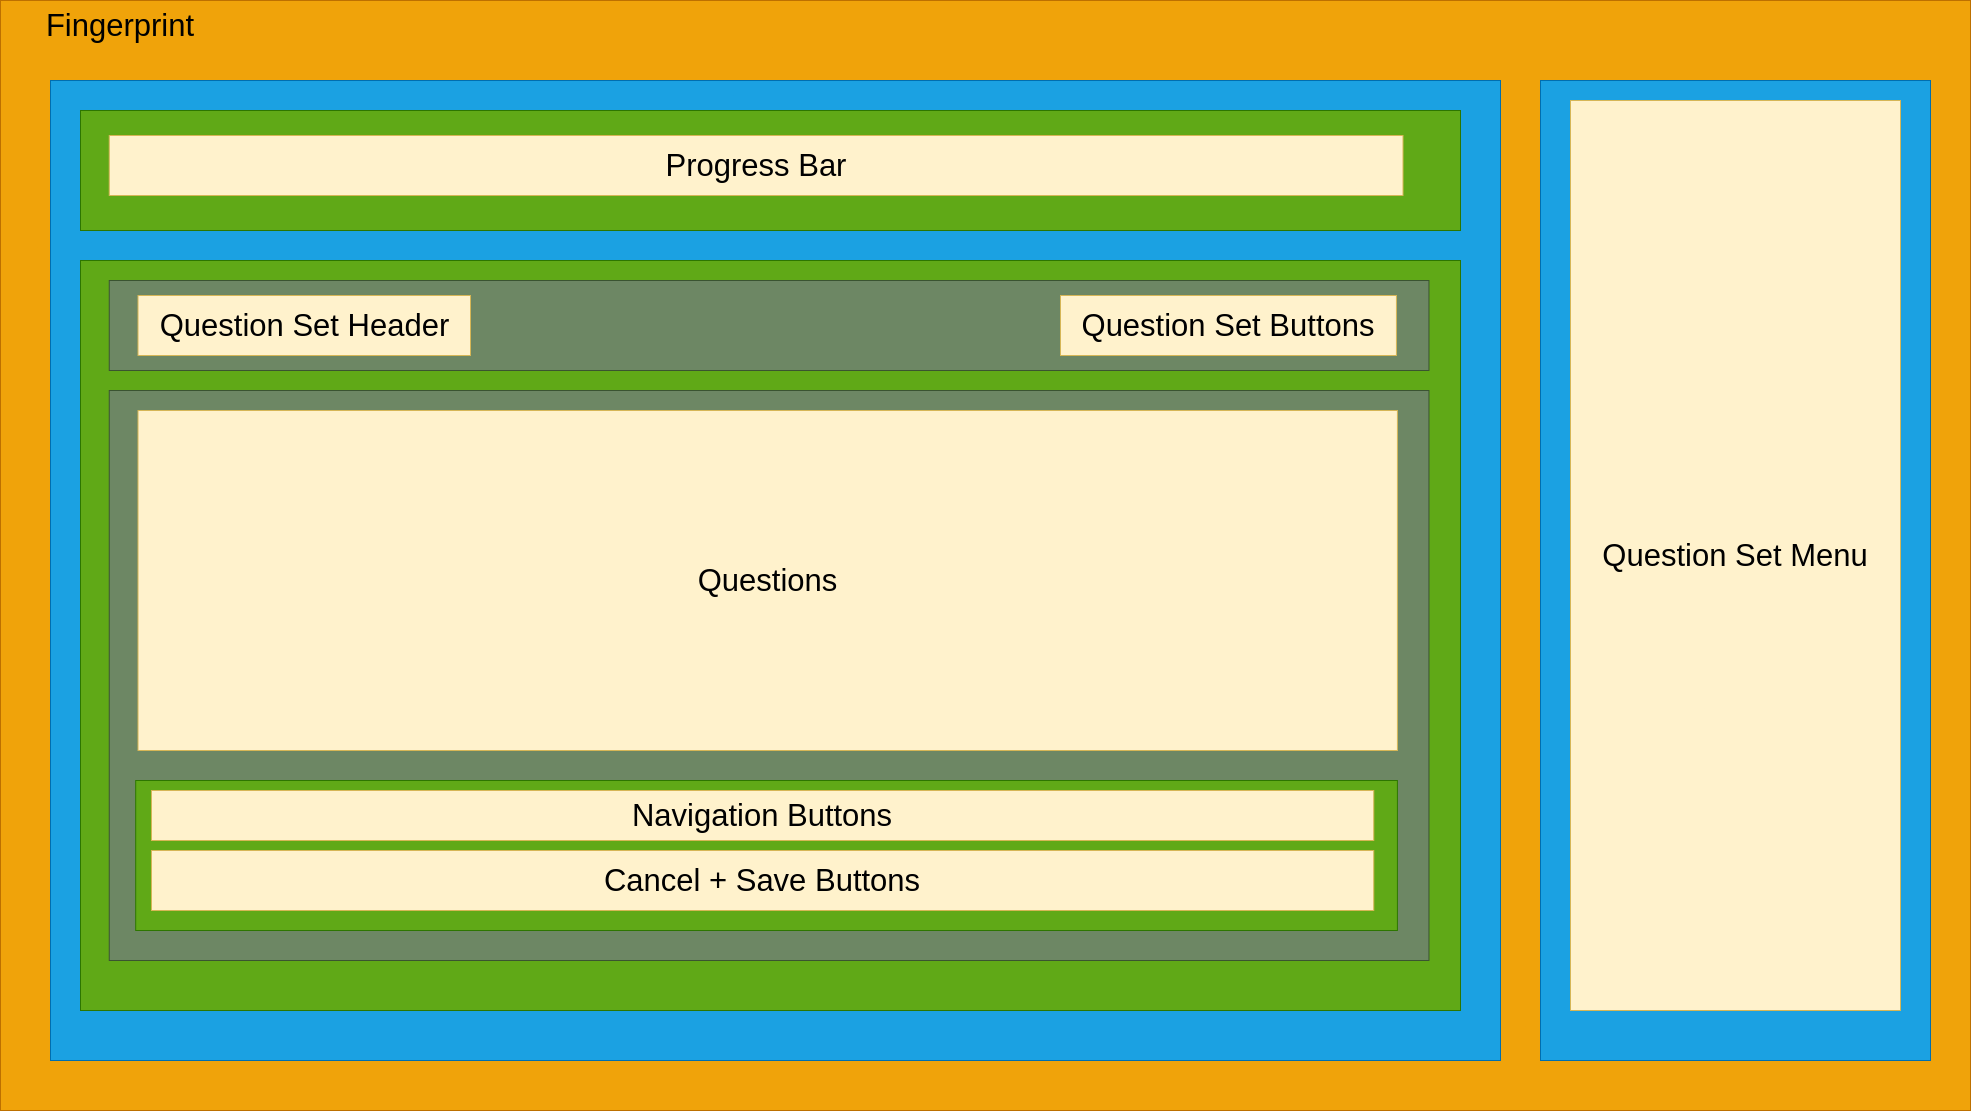
\includegraphics[width=\textwidth]{fingerprint-other-after-diagram}
    \caption{New fingerprint template for the create, edit, search and preview fingerprint views variations.}
    \label{fig:fingerprint-other-after-diagram}
\end{figure}

The show variation, as shown in figure \ref{fig:fingerprint-show-detailed-after-diagram}, uses a single column with two rows layout.
Previously the show variant had no Question set buttons, however, to keep consistency with the other variants, the Collapse and Show buttons were moved to the Question Set Buttons where they were being displayed on the other variants.
By default, the only button visible on the Questionnaire buttons is the Summary, which will hide the current detailed view and show an alternative summary layout, where answers are displayed in several tables, one for each question set.

\begin{figure}[H]
    \center
    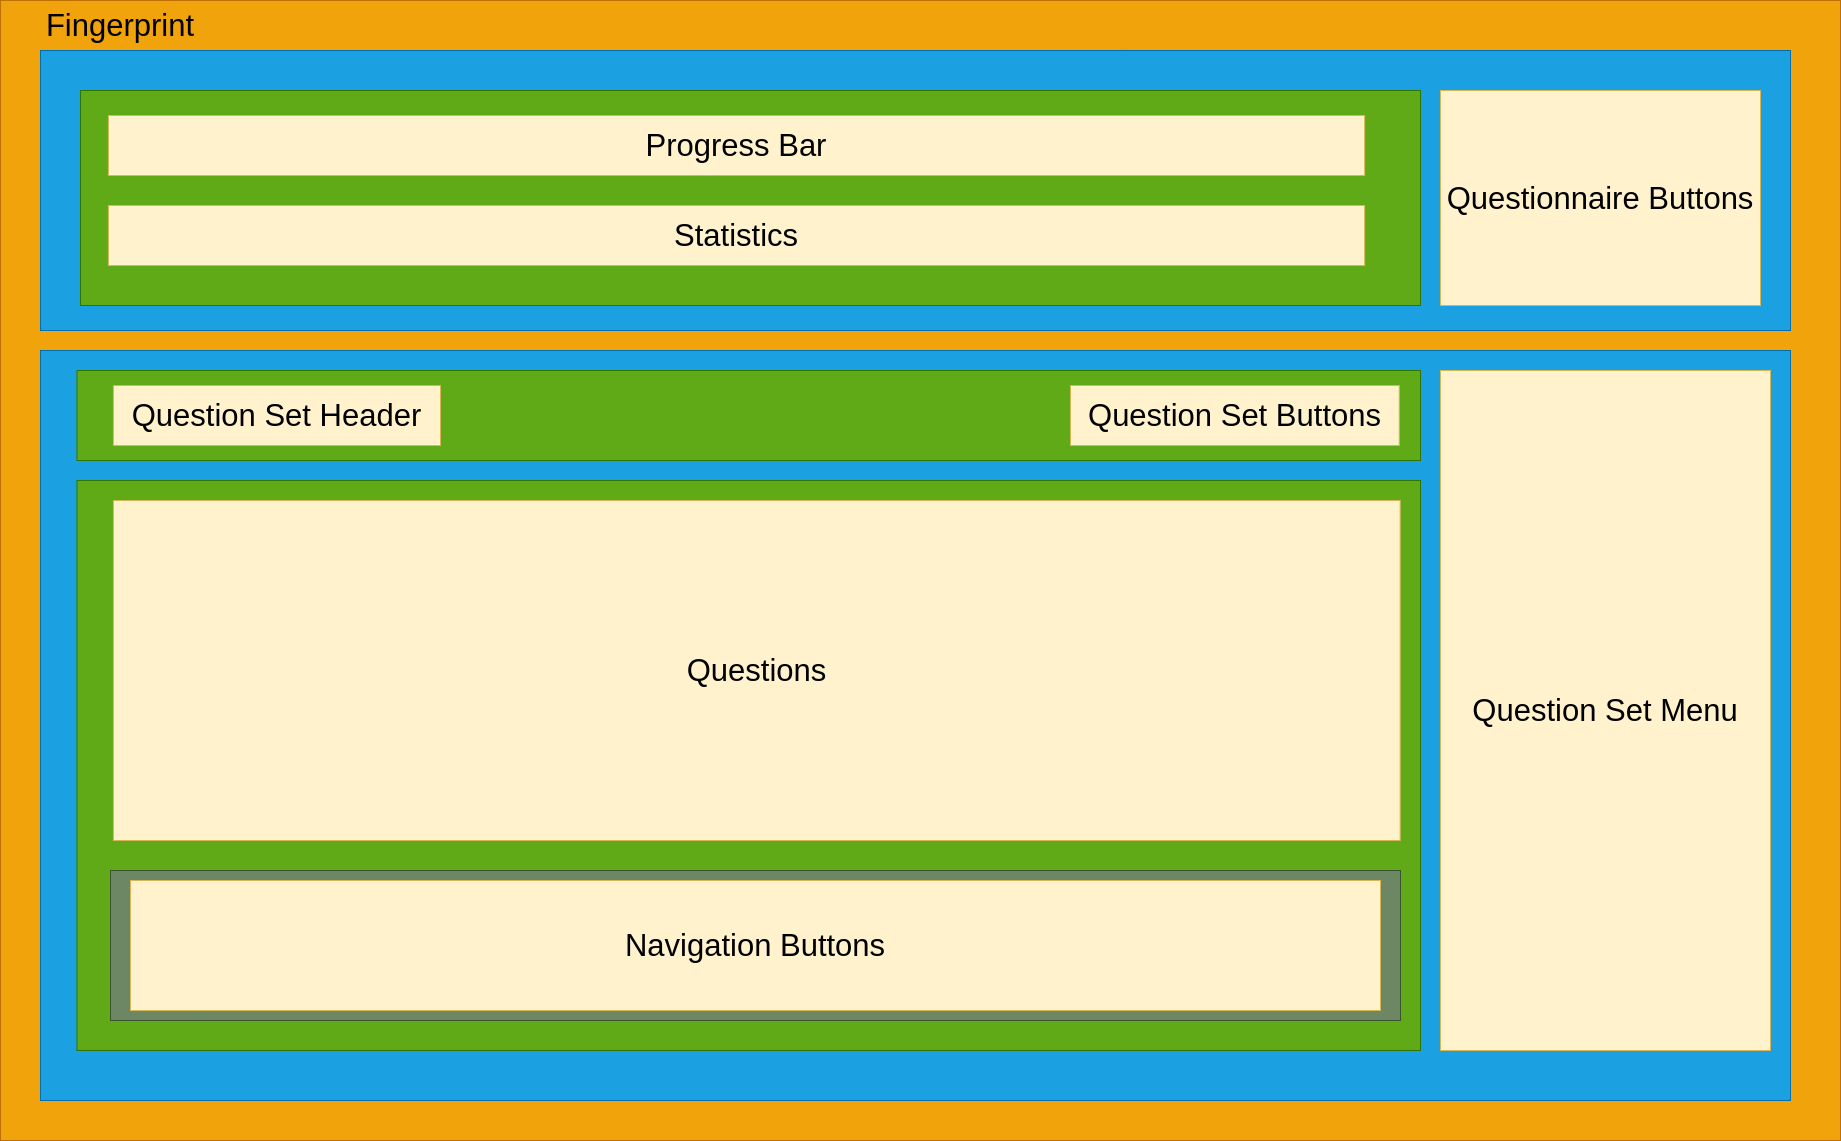
\includegraphics[width=\textwidth]{fingerprint-show-detailed-after-diagram}
    \caption{New fingerprint template layout for the detailed show fingerprint view variation.}
    \label{fig:fingerprint-show-detailed-after-diagram}
\end{figure}

As can be observed in figure \ref{fig:fingerprint-show-summary-after-diagram}, when the user switches to the summary view, by clicking on the Summary Questionnaire button, the detailed view container is hidden, and the summary view container is displayed.

\begin{figure}[H]
    \center
    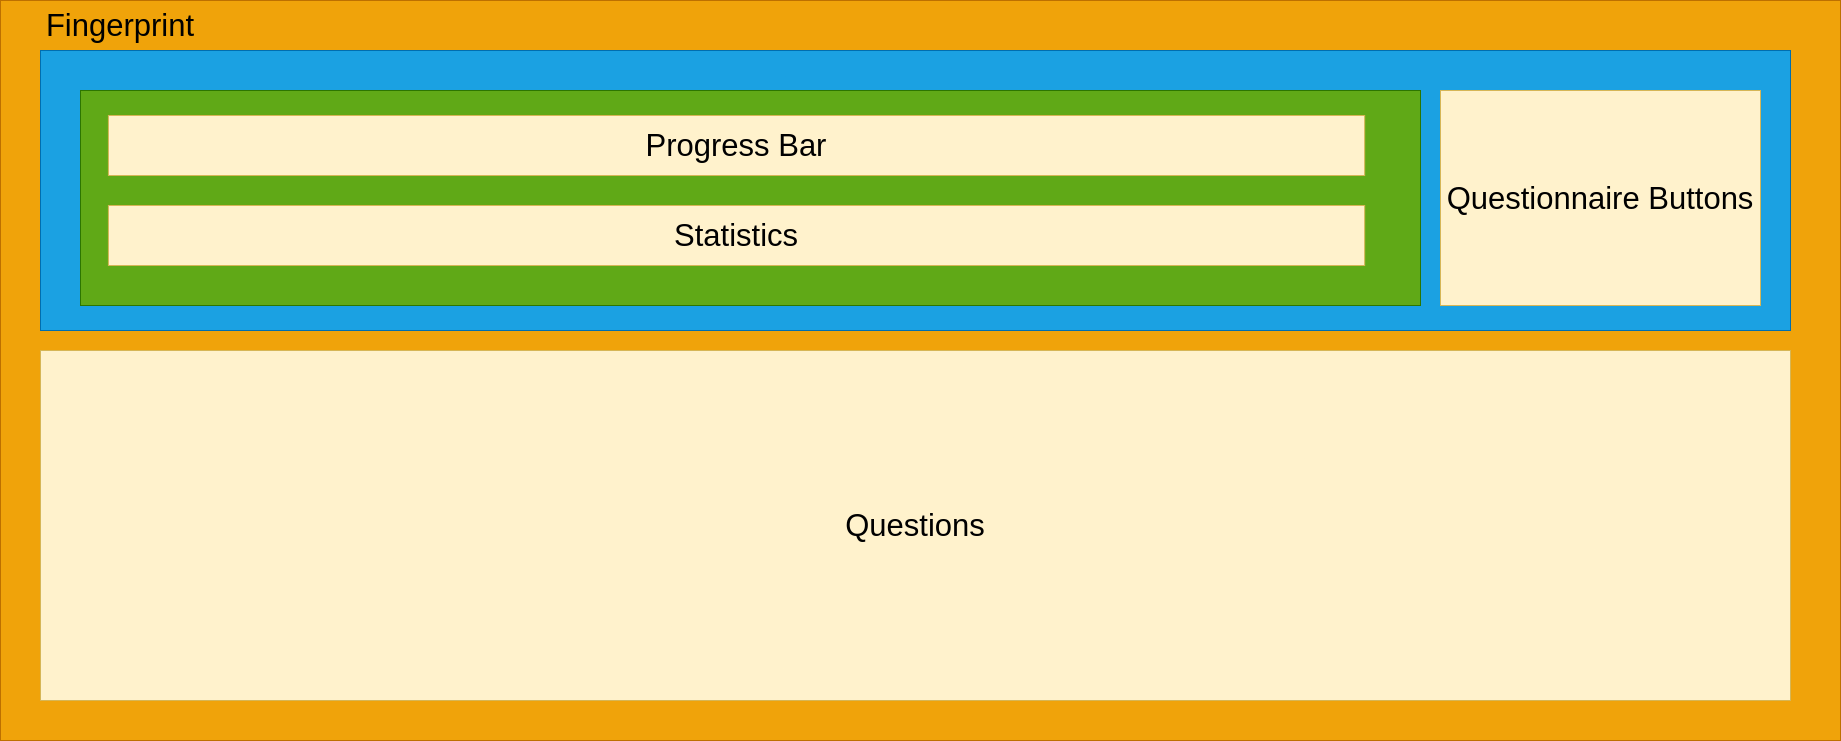
\includegraphics[width=\textwidth]{fingerprint-show-summary-after-diagram}
    \caption{New fingerprint template layout for the summary show fingerprint view variation.}
    \label{fig:fingerprint-show-summary-after-diagram}
\end{figure}

It is important to note again that the overall aesthetics and workflow of the page were not changed.
The only major change was to divide the fingerprint view into several, reusable components.

When we went over how question sets were rendered, we saw that each question set had its container and they are only rendered when is accessed for the first time.
When it needs to be rendered, \gls{api} endpoints are used to fetch the \gls{html} of a specific question set.
On this \gls{html} returned, each question had attached their client-side validation code.
The goal is to remove all existing code of client-side validation, making use of only simple built-in \gls{html} validations on the client-side and use Django's forms framework to have all remaining validations on the server-side.

Before going into more details let's go over Django's built-in form system and some of its components.
A form in \gls{html} is represented through the form tag and fields are represented through input tags.
Each input tag has a type attribute that defines how the data will be inserted by the users, for example, to insert a date the user will be presented with a calendar where it can click on the desired date.
These different ways to insert data are called widgets.
To work with forms, Django only makes use of two \gls{http} request methods: GET and POST.
GET is used by browsers to fetch the page/\gls{html} of an URL and it can also be used to fetch information.
POST on the other side is used to send information to a server.
On the backend side, Django has three main classes that handle the data around forms.
The main one is the \textit{Form} class that defines how it works and how it will be presented to the user.
Then there is the \textit{Field} class that describes a field of a form, which is in charge of performing field-specific validations.
Django already has some implementations of this class for the most common field types such as number, text, choice, \dots
Finally, the \textit{Widget} class is in charge of processing and transforming the raw data received and also preparing and restructure data to be presented to the user, and again Django already has some implementations of this class.
Each \textit{Field} class has a widget class associated.
The common development flow is to create a child class of Django's \textit{Form} class and then define its fields with \textit{Field} classes.

However, in the case of MONTRA, the number and type of the fields are dynamic, since both can be customizable by a community manager when he is building a questionnaire.
A Submission form was created, child of Django's \textit{Form} class, where its constructor was overridden so the fields of the requested Question Set of a Questionnaire are defined in the form class.
Additionally, several question types lead to the need of having to create and associate new \textit{Field} and \textit{Widget} child classes since they were too complex to be represented or validated with the ones that Django already has implemented.
To build the widgets of such question types, existing implementations were ported to an associated Django template to then be used in its new widget class.

By removing all validations from the front end, client-side code is now only used to make \gls{api} calls to the backend, to validate the data inserted by the user, and to add functionality to the page itself, such as hide and/or show elements on the page after a button is clicked.
All client-side code related to the fingerprint was either migrated or newly implemented using, as much as possible, plain javascript, avoiding any external library.
It avoids adding yet another dependency to the project, and if in the future, upgrades are done to libraries such as JQuery\footnote{https://jquery.com/}, the code implemented here is not affected and does not require any refactoring.

\subsection{Programming interface}
% UI changes
% consequencia da alteração do front end devido à alateração do backend
% passar toda a verificação para o backend, passando a usar a validação built in do Django
% tentar reutilizar os modulos existentes

As all the validations were moved to the backend, it was necessary to create several \gls{api} endpoints that perform them.
Such validations take advantage of Django's form system, so in the implementation of each endpoint, it is only necessary to build a SubmissionForm then add the data provided by the user and then call its validation method, which will validate all the fields that were defined in the form.

Besides the user input validation, there need to be new endpoints that render the \gls{html} of a question set of a questionnaire using the new questions models and Django's forms system.
As different fingerprint view variations might present the questions and answers differently, there are different endpoints for each fingerprint variant:

\begin{lstlisting}[basicstyle=\tiny]
GET  [base url]/questions/[questionnaire id]/[section index]/preview/

GET  [base url]/questions/[community slug]/[questionnaire id]/[section index]/search/

GET  [base url]/questions/[community slug]/[questionnaire id]/[section index]/create/
GET  [base url]/questions/[questionnaire id]/[section index]/create/

GET  [base url]/questions/[fingerprint hash]/[section index]edit/

GET  [base url]/questions/[fingerprint hash]/[section index]/show/
\end{lstlisting}

There are two different endpoints for the create variant, because certain installations are a single community, for that, the community is implicit, but for multi-community installations, the community slug is required, since the same questionnaire can be used on different communities.

For the edit and create variants, there need to be additional endpoints that are in charge of performing all the validations associated with each field and saving the progress when the user changes from one question set to another if no error is found.
Bellow are such:

\begin{lstlisting}[basicstyle=\scriptsize]
Submissions Management:
POST [base url]/api/submission/save/[community slug]/[questionnaire id]/[section index]/
POST [base url]/api/submission/save/[questionnaire id]/[section index]/
PUT [base url]/api/submission/save/[fingerprint hash]/[section index]/

Questionnaire Information:
GET  [base url]/api/questionnaire/info/[community slug]/[questionnaire id]/[section index]/
GET  [base url]/api/questionnaire/info/[questionnaire id]/[section index]/
\end{lstlisting}

Related to the Submissions Management endpoints, which are used to save answers data, the first two endpoints follow the same idea as the ones presented before, which on single community installations there is no need to provide the community slug.
However, there is a third alternative.
The first two should be used when there is not yet a fingerprint created, and which will return both the fingerprint hash of the created fingerprint and the current submission token.
The fingerprint hash is the identifier of a fingerprint, the submission token is used to identify if different calls to the save endpoints are related to the same changes.
With that, several changes can be grouped in the same Submission, instead of the previous implementation that would create a FingerprintHead record for each save of a question set.

This also enforces that if the user performs several changes to the same question set with the same submission token, only the last changes will be kept, replacing (figure \ref{fig:submissions-new-answer2}), or even deleting (figure \ref{fig:submissions-remove-answer}), old answer values sent in the same submission.

\begin{figure}[H]
    \center
    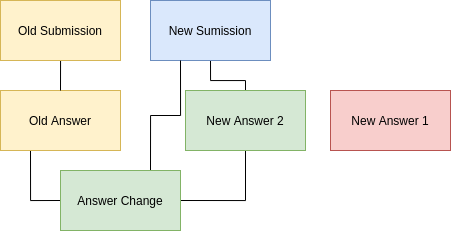
\includegraphics[width=.5\textwidth]{submissions-new-answer2}
    \caption{When an answer change is submitted and there were already changes made to that question, then the previous one is deleted (New Answer 1) and a new one (New Answer 2) is associated with both the current Submission and the related Answer Change.}
    \label{fig:submissions-new-answer2}
\end{figure}

\begin{figure}[H]
    \center
    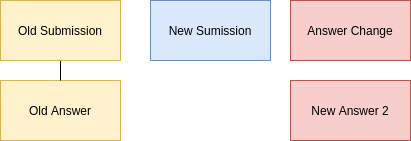
\includegraphics[width=.45\textwidth]{submissions-remove-answer}
    \caption{If the user either provides an empty value or no value to an answer that previously had a value on the current submission, associated Answer and Answer Change records are deleted.}
    \label{fig:submissions-remove-answer}
\end{figure}

If no submission token or one that does not match the current one is provided, then it is assumed that the changes submitted are related to a new submission, thus the most recent submission is closed and the new provided answers are added to a new submission.

\begin{figure}[H]
    \center
    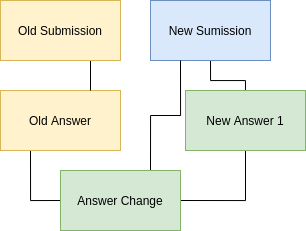
\includegraphics[width=.3\textwidth]{submissions-new-answer}
    \caption{Whenever new changes to the answer of a question in a specific submission are submitted, a new Answer model is created, and also an Answer Change record is created connecting with the previous answer.
In the case the provided submission token does not match the current one stored in the fingerprint model, then a Submission record will also be created, and changes will be associated with this new Submission.}
    \label{fig:submissions-new-answer}
\end{figure}

Previously it was possible to update an answer of a single question through endpoint \textit{/api/fingerprints/[fingerprint hash]/answers/[question slug]/}, mentioned in the \gls{api} portion of section \ref{sec:fingerprints}, which was a more user-oriented alternative to the ones that were used on the old fingerprints views.
On the new endpoints to validate and save the answers of a question set, if a single answer is sent, Django's form system will consider the rest of the answers to the other questions of the question set as empty.
With this, the user is forced to always send the previous answers to all other questions plus the updated answer of the specific question.
To avoid this, the \textit{/api/fingerprints/[fingerprint hash]/answers/[question slug]/} endpoints were kept, refactoring them to use the new models and Django's form system, but in these, the form used to perform the validation only contains one question instead of all questions of a question set.

With all this changes to the endpoints, choice-based answers are stored as a foreign key to the choice(s) selected.
This implies that the answer's data sent on the Submissions Management endpoints for such question types must be these foreign keys, avoiding misspellings and non-existing choices.
However, one does not know the keys for each choice and also the available choice if the web view is not used.
For that, the Questionnaire Information endpoints are used to get information of choice-based questions, so that the correct data is sent along with the Submissions Management endpoints.

\subsection*{Draft Status API}

There were also some modifications to the endpoints to change the publish status of a fingerprint.
Instead of having two different endpoints for different community settings (to auto-accept or not fingerprint publish requests), but for the same purpose, now only one exists.

\begin{verbatim}
POST [base url]/api/draft/[fingerprint hash]
\end{verbatim}

This endpoint expects the same data in the same format, though takes different actions according to the community of the fingerprint at issue.
Also, on the previous versions of publishing endpoints, there was a possibility to publish fingerprints that were not complete, not having answers to required answers.
Now, a validation is implemented when the user wants to publish its fingerprint, not completing the change on the publish status if the fingerprint is not complete.
This avoids notifications being sent to the community manager telling that a user wants to publish a fingerprint, although such fingerprints might be incomplete.

\subsection{Excel}
% mais concreto, e tem mais em conta o contexto em volta das questoes
% entanto é mais estenso
% tipos de perguntas novos e deprecated

The previously presented version of the spreadsheet used to define a questionnaire, had some problems in terms of clutter due to the overuse of the ``Value list'' column to define the extra configuration of specific questions types.
The column was used to define all choices and their extra information of choice-based questions, to define columns and their settings of open multiple question and columns, rows, and type of choice tabular questions.

To fix those clutter problems, improvements were done to the spreadsheet by deleting some useless columns that were related to deprecated features and adding new types of rows that define the extra configurations for those questions types that require.

Starting by the columns of the actual spreadsheet now are the following:

\begin{itemize}
    \item Type;
    \item Text/Question;
    \item Data Type;
    \item Help Text/Description;
    \item Slug;
    \item Dependencies;
    \item Constraints;
    \item Tooltip;
    \item Include in Advanced Search.
\end{itemize}

Most of the columns are already known from the previous version, ``Constraints'' being the only one that was added to this new version.
The columns that were removed are Stats, Comments Stats, Disposition (all associated with deprecated features), Level/Number (the number is now automatically retrieved according to the order of how the rows are defined), and Value List (brought the clutter problem to the table).

\subsection*{Type}

On this column, the only possible values available were QuestionSet, Question, and Category.
The new version has now eleven possible types of rows for the spreadsheet:

\begin{table}[H]
\centering
    \begin{tabular}{| p{.2\linewidth} | p{.8\linewidth} |}
\hline
\textbf{Type}                 & \textbf{Description}                                                                       \\ \hline
\multirow{2}{*}{IntroSection} &
  \multirow{7}{=}{These represent the same concept as QuestionSet. \\ In the previous version, it was possible to add hidden question sets to both the beginning of the end of the questionnaire. This was achieved by setting the Level/Number column to either 0 or 99 respectively. Since the Number portion of that column was removed, such Question Sets must be represented with the IntroSection and CloseSection rows.} \\
                              &                                                                                            \\ \cline{1-1}
\multirow{3}{*}{Section}      &                                                                                            \\
                              &                                                                                            \\
                              &                                                                                            \\ \cline{1-1}
\multirow{2}{*}{CloseSection} &                                                                                            \\
                              &                                                                                            \\ \hline
Group                         & This is a replacement to the category row type plus the comment question type.             \\ \hline
Question                      & The old and unchanged Question row type                                                    \\ \hline
Choice                        & This row indicates a choice of the previously defined Question                             \\ \hline
ChoiceInfo &
  Allows adding an extra question that can be answered if a specific choice is selected. Such a question will be rendered right below the choice.

        Note that this is different from the dependencies column. \\ \hline
TabularChoice                 & \multirow{2}{*}{Row types to define the configuration of choice tabular question types}    \\ \cline{1-1}
TabularRow                    &                                                                                            \\ \hline
Column                        & \multirow{2}{*}{Row types to define the configuration of the open multiple question types} \\ \cline{1-1}
ColumnChoice                  &                                                                                            \\ \hline
\end{tabular}
\caption{Available values to use on the ``Type'' Column of the new version of the spreadsheet to define a questionnaire.}
\label{tab:excel-row-types}
\end{table}

Using the new row types described in table \ref{tab:excel-row-types}, the spreadsheet itself will be longer, however, it will be easier to read.
In figures \ref{fig:choice-tabular-neu}, \ref{fig:open-multiple-neu} and \ref{fig:choice-neu}, it is presented three before and after of how questions that require extra configuration were and are now defined with the new spreadsheet version.

\begin{figure}[H]
    \center
    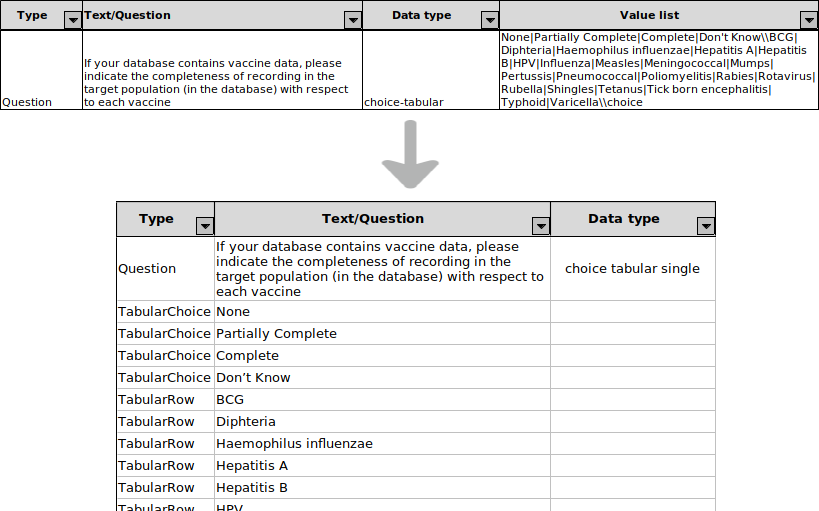
\includegraphics[width=.75\textwidth]{choice-tabular-neu}
    \caption{Differences between how a choice tabular question was versus how is now defined on the questionnaire spreadsheet.}
    \label{fig:choice-tabular-neu}
\end{figure}

\begin{figure}[H]
    \center
    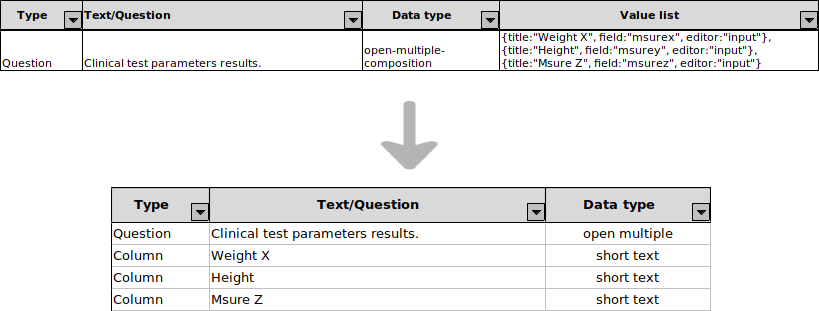
\includegraphics[width=.75\textwidth]{open-multiple-neu}
    \caption{Differences between how a open multiple question was versus how is now defined on the questionnaire spreadsheet.}
    \label{fig:open-multiple-neu}
\end{figure}

\begin{figure}[H]
    \center
    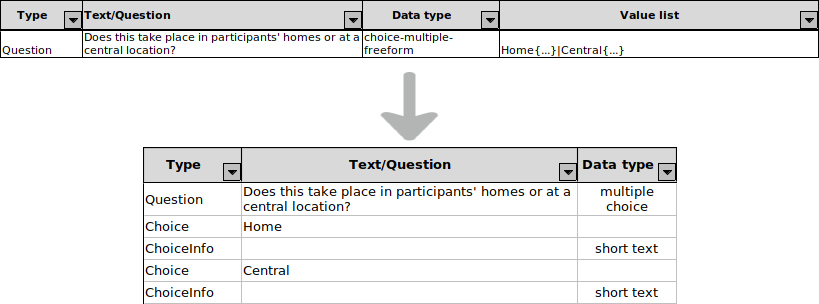
\includegraphics[width=.75\textwidth]{choice-neu}
    \caption{Differences between how a open multiple question was versus how is now defined on the questionnaire spreadsheet.
    Note that now it is possible to specify the data type of the extra information that is attached to the extra information of a choice.}
    \label{fig:choice-neu}
\end{figure}

It was considered to also remove the Level part of the Level/Number column, adding an EndGroup row type.
Then whenever the user wanted to create a subgroup of questions after a question would create a Group with empty text and the framework would move the question of that group to a deeper level with no group label.
This however would make the spreadsheet even longer for certain questionnaires that make use of categories to group questions that have some dependency on another question.
Figure \ref{fig:excel-end-group} shows how the change would affect the spreadsheet.

\begin{figure}[h]
    \center
    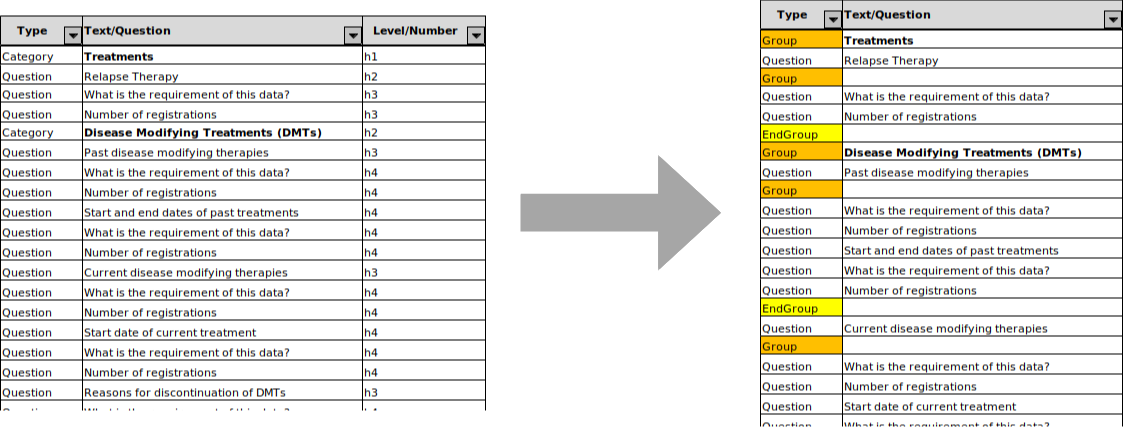
\includegraphics[width=\textwidth]{excel-end-group}
    \caption{A possible solution to avoid relying on the Level column to create subgroups of questions. On the new solution proposed it is much difficult to know at which level the specific question is located, without looking at the rows above.}
    \label{fig:excel-end-group}
\end{figure}

Even with colors, the user editing has to look several rows above to know at each level it is so he can match the ``EndGroud'' rows with the respective ``Group'' rows.
This is the same problem as matching if open and closing brackets on C-like programming languages.
Such a problem is alleviated since indentation is allowed, which can not be achieved on a spreadsheet.
For those reasons, the Level column was kept, however, when a questionnaire is imported, whenever there are nested levels the framework will create groups with empty text.

\subsection*{Data Type}

As it was possible to see in figures \ref{fig:choice-tabular-neu}, \ref{fig:open-multiple-neu} and \ref{fig:choice-neu}, the Data Type column is used to detail the type of data that will be stored and how it will be requested to the user in terms of HTML widgets.

Table \ref{tab:original-question-types} contains all the previously allowed question types, a total of twenty-five different types.
On the new version, this list was reduced, where some questions can now be achieved using simple question types in conjunction with the new row types that extend their base functionality.

Next is the list of question types available after the refactoring:

\begin{itemize}
    \item short text: Old open. It replaces the open-validated field by making use of the new Constraints column;
    \item long text: Old open-textfield;
    \item single choice: Used to achieved any old single-choice question type. The extra information input can now be achieved with the ChoiceInfo row type;
    \item multiple choice: Used to achieved any old multiple-choice question type. The extra information input can now be achieved with the ChoiceInfo row type;
    \item integer: Old integer;
    \item date: Old datepicker;
    \item email: Old email;
    \item url: Old url;
    \item numeric: Old numeric;
    \item publication: Old publication;
    \item image: Old open-upload-image;
    \item choice tabular: Old choice-tabular;
    \item open multiple: Can achieve both the old open-multiple and open-multiple composition.
\end{itemize}

Open-location and timeperiod were removed since they were not being used on any of the active installations of the MONTRA framework.
The same happened with sameas and custom as additionally, they were shortcut type questions.

\subsection*{Slug and Dependencies}

Previously the dependencies between questions were detailed by providing the id of the target question and the order of the choice that was needed to be selected, but since now the choices are described by row, the user can also detail an id for them, which such id can then be used on the Dependencies column of the questions that depend on such choice.

\subsection*{Constraints}

The old Question model allowed to add custom checks, however, this feature was not possible to make use of through the spreadsheet, it was only possible to define them after the questionnaire was imported.
This ``Constraints'' column intends to enable configuring such additional checks.
Checks were previously stored in a custom format, where each check was separated by a space, defined as $name="value"$.
To avoid having to parse a string every time we want to load the constraints, they are now stored in a \gls{json} field.
Regarding the spreadsheet, the format chosen was a modified version of the original checks, supporting several types instead of interpreting every value as a string, allowing flexibility on the whitespace between each and within a check.
Next is presented some examples:

\begin{verbatim}
name: "value"  -> string
name: true     -> boolean
name: 1        -> integer
name: 1.5      -> numeric
name: value2   -> also a string
\end{verbatim}

\gls{json} was also considered, however it was too much verbose to put on a spreadsheet cell, emerging the clutter problem.

Currently, the supported constraints are the following:

\begin{table}[H]
\centering
\begin{tabular}{|l|l|}
\hline
\textbf{Question Type(s)}                                                       & \textbf{Constraint} \\ \hline
any                   & required    \\ \hline
\multirow{3}{*}{\begin{tabular}[c]{@{}l@{}}short text\\ long text\end{tabular}} & min\_length         \\ \cline{2-2}
                      & max\_length \\ \cline{2-2}
                      & regex       \\ \hline
\multirow{2}{*}{\begin{tabular}[c]{@{}l@{}}integer\\ numeric\end{tabular}}      & min\_value          \\ \cline{2-2}
                      & max\_value  \\ \hline
\multirow{3}{*}{date} & min\_date   \\ \cline{2-2}
                      & max\_date   \\ \cline{2-2}
                      & format      \\ \hline
\end{tabular}
\caption{Newly available constraints to apply to a question.}
\end{table}


\section{Summary}
In this chapter, a metadata storing and visualization tool, the MONTRA framework, was detailed and analyzed, highlighting some of its poor design choices, which impact its usability and maintainability.
A refactoring process was performed to fix such problems, preventing and giving feedback on user error when submitting data and improving the overall maintainability of components related to the metadata displaying.

The next chapter will go over the remaining part of the process regarding metadata.
Extracting it from a database and then send it to update tools that store and display it, such as an installation of the MONTRA framework.

\chapter{Automatic Metadata Extraction and Update}
\label{chapter:extraction-update}
\graphicspath{{figs/04-extraction-update/}}

As we have an application ready to receive and display metadata, it is now crucial to turn the attention to extracting metadata from \gls{cdm} databases, which contain the actual data, allowing, then, to update the data stored on applications such as the MONTRA framework.

Figure \ref{fig:overall-arch-v1} presents a high-level architecture of the desired system that extracts data from databases and sends it to the applications that need their local data updated.
Agents are software that runs on the data owner's deployment, in charge of extracting metadata from the database and sending this metadata to the applications.

\begin{figure}[H]
    \center
    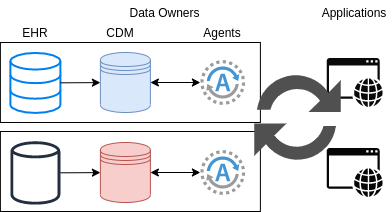
\includegraphics[width=.6\textwidth]{overall-arch-v1}
    \caption{High-level architecture of the extraction and update process.}
    \label{fig:overall-arch-v1}
\end{figure}

\section{Requirement Analysis}

When we enter the realm of accessing an institution's sensitive data, some problems start to arise.
Not all data owners are willing to, or legally can't, provide direct access to their data.
When building this part of the system, we have to consider this and have several options available that use different levels of access and according to the demands of each specific data owner, use the most appropriate one.
In one end, a single solution could have full access to the data, extracting the metadata directly from the original data.
At the other end of the scale, the burden of extracting data is removed from us and the system is dependent on the data owner providing the metadata and only then the system processes the metadata.
Having several options for different access levels is more flexible, however, it requires maintaining several tools which are not reliable.
A more appropriate alternative is to have a single option, that is designed considering the most strict access to the data, however, we still need to provide a tool to extract the metadata.
The only difference is that we are not the ones executing it.

As the extracting tool has direct access to the data, using an existing and widely known tool is a must, so data owners are inclined to use it.
Additionally, making fewer to no changes is preferable to ensure that data owners don't discard the tool because they don't trust the changes.

\begin{figure}[H]
    \center
    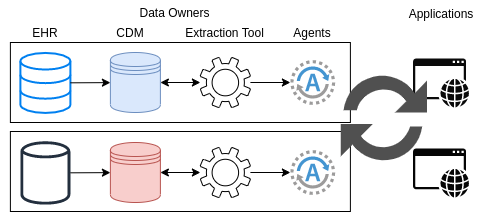
\includegraphics[width=.6\textwidth]{overall-arch-v2}
    \caption{High-level architecture of the extraction and update process}
    \label{fig:overall-arch-v2}
\end{figure}

In figure \ref{fig:overall-arch-v2} is presented the overall architecture of the system, where the agent is the tool in charge of parsing the metadata provided by the data owner, which is then sent to the applications.
Regarding this last point, there needs to be a way for the data to go from the agents to the applications.
One ambitious solution is to create a decentralized peer-to-peer network of agents, avoiding developing a central component.
In such solution, the agents are in charge of managing and sending the data to the applications.
However, data owners might not want to spend their hardware resources to maintain a network.
Since the agents are executed on the data owner's system, they should do only the required and minimal functionality, spending the few resources as possible.

A more executable solution is to have an intermediate component that receives the metadata from the agents and then distributes that data across the applications, following a centralized network architecture as it is presented in figure \ref{fig:overall-arch-v2}.

\begin{figure}[H]
    \center
    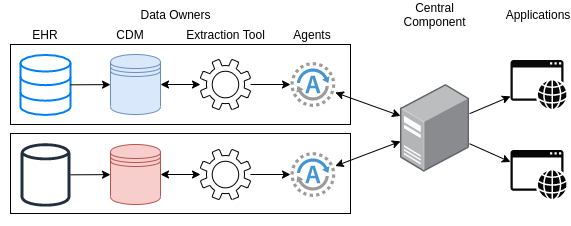
\includegraphics[width=.6\textwidth]{overall-arch-v3}
    \caption{High-level architecture of the extraction and update process, with a centralized network approach.}
    \label{fig:overall-arch-v3}
\end{figure}

This central component will be used to manage the data and the applications to where such has to be sent.
However, it is also crucial that feedback is provided on the system's state, such as how the data is flowing, which applications received which data, and which databases sent data into the system.

% aqui digo que percisamos de um componente intermedio. mais á frente vou dizer que percisamos um componente intermedio entre o kafka e as aplicações. coisas diferentes

On the applications side, there are other important factors to consider before going forward on implementing the intermediary component mentioned before.
First, then we talk of application we are considering only web application that expect to receive metadata through a \gls{rest} \gls{api}.
Second, the \gls{api}s of different applications expect the metadata in distinct arrangements.
A way out of this would be to specify a set of endpoints that each application had to implement, yet that would lead the applications to have two sets of endpoints that do the same thing.
On the other side, making a flexible option, where the requests where the data is sent are customizable, would be more appealing for the target applications, which would not have to make any changes.
Third, not all applications require all metadata data that is extracted from a database.
Some use all the data, others only need a value of such data.

\subsection{Functional Requirements}

\begin{enumerate}
    \item Databases must be registered on the central component
        \begin{list}{}{}
        \item By having a record of the databases that are attached to the network, the system can avoid accepting data from databases that were not registered in the system.
        \end{list}

    \item It must be possible to check what agents are active at a certain point
        \begin{list}{}{}
            \item This allows giving feedback on the state of the network to the admin.
        \end{list}

    \item The system should allow managing the destination applications
        \begin{list}{}{}
            \item The applications to where the data of the databases are sent, should not be hard-coded, for that, the network admin should be able to perform \gls{crud} operations on such.
                The term application should be interpreted as web applications that have \gls{rest} \gls{api} endpoints available to receive data.
        \end{list}

    \item The system should provide statistics on the data that has circulated
        \begin{list}{}{}
            \item This is yet another feature to give feedback to the network admin about, now allowing to both check the amount of data that each database sent, and the amount of data that each application received.
        \end{list}

    \item The format of the request sent with the metadata to each application must be customizable
        \begin{list}{}{}
            \item This is important since different applications expect to receive metadata in distinct formats since each application has a different \gls{api}.
        \end{list}

    % eu não falo aqui das pipelines, que permitem filtrar os dados, pk isso foi algo que adicionei como consequencia consequencia em termos usado kafka

    \item The system should allow to group Databases
        \begin{list}{}{}
            \item In a scenario where both all the destination applications and all databases belong to the same project, the metadata of the databases makes sense in all applications.
            \item Now consider a scenario where half of the databases are associated with one project and the rest with another.
          Each project has a destination application that receives the data.
          Considering that there is no concept of project or groups, both applications will receive data of both projects.
          To solve this, it required to have two installations of this system, one for each project.
          By grouping databases, data of a database can be guided to applications that are also attached to the same group.
        \end{list}

\end{enumerate}

\subsection{Non-Functional Requirements}

\begin{enumerate}
    \item The data owner can stop the agent at any time
        \begin{list}{}{}
            \item This was also applied in \cite{gaain}.
                It gives yet another layer of control to the data owners over their data.
          If at any time, they don't want to share their data, they can stop the agent.
          This also poses a constraint in the system that it should not be designed assuming that the agents, once deployed, will always stay active.
        \end{list}

    \item The extraction tool should be based as much as possible on an already existing solution
        \begin{list}{}{}
            \item Using a working solution avoids having to build a new tool from scratch.
              But apart from that, using a known solution as a base helps to gain the confidence of the data owners so that they use the resulting solution in their databases.
        \end{list}

    \item The agents must not have direct access to the data
        \begin{list}{}{}
            \item This option assumes the least amount of access to the user's data so data owners are receptive to allow agents to be run on their local deployments.
              This will require that an agent has access to at least a shared storage where agents check for new data and data owners post their extracted metadata.
        \end{list}

    \item The agent should easily deployable
        \begin{list}{}{}
            \item As the installation of the agent will be done by a person not familiar with the project, this process should be as smooth as possible and well documented.
        \end{list}

    \item Agents should spend few resources
        \begin{list}{}{}
            \item Considering agents run on data owners' deployment environment, it should have a low resource footprint so it does not impose any disruption.
              For that, they must be designed to perform only the required task.
        \end{list}

    \item The system should not require any open ports on the data owners' deployment environment
        \begin{list}{}{}
            \item As there might be communication between the central component and the agents, requesting an open port on the data owners' deployment environment might not be possible since it could require them to change firewall settings as was mentioned in \cite{popmednet}.
        \end{list}

    \item Scalable
        \begin{list}{}{}
            \item As more databases are connected to the network, the system should allow increasing resources so that it handles processes faster.
        \end{list}

    \item Microservice architecture
        \begin{list}{}{}
            \item The system should be composed of simple and replaceable components that deal with well-defined tasks.
        \end{list}
\end{enumerate}

\subsection{Use Cases}

From the previous requirements defined, there can be outlined two actors that will interact with the system:

\begin{itemize}
    \item Data owners, which maintain the agent on their local deployment;
    \item System admin, that interacts with the central component to manage the whole system.
\end{itemize}

In figure \ref{fig:use-cases} is presented the use-case diagram, which shows the actions that each actor performs on the system.
Such actions were divided into three groups: Agents, Metadata Extraction, actions on the central component related to receiving data from the agents, and Metadata Update, actions on the central component related to sending data to the applications.

\begin{figure}[H]
    \center
    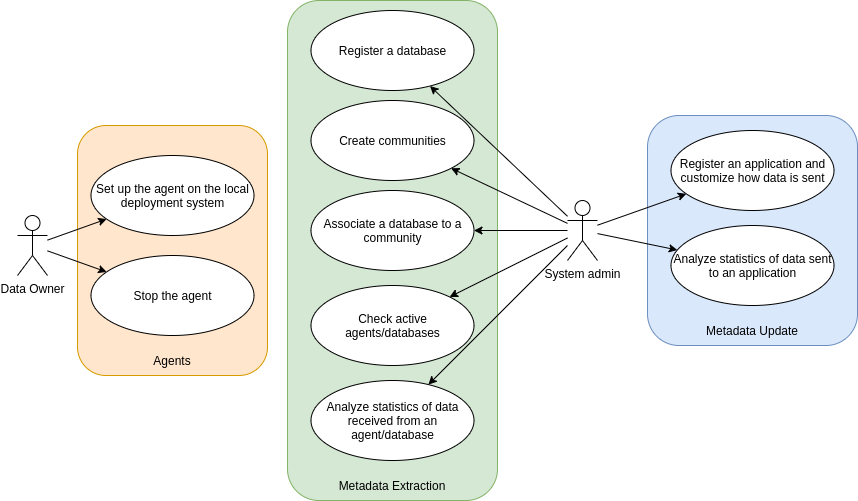
\includegraphics[width=\textwidth]{use-cases}
    \caption{Use case diagram of the metadata extraction and update system}
    \label{fig:use-cases}
\end{figure}

\begin{enumerate}
    \item Set up the agent on the local deployment system
        \begin{list}{}{}
            \item Since it's not expected that data owners provide access to their deployment environment, the responsibility to set up the agent is imposed on them.
        \end{list}

    \item Stop the agent
        \begin{list}{}{}
            \item As Data owners control their data and the access to it at all times, them stopping the agent should be an action expected by the system.
        \end{list}

    \item Register a database
        \begin{list}{}{}
            \item As new databases enter the network and agents are deployed to gather their metadata, the system admin needs to register new databases on the central unit, so the data received is accepted into the system.
        \end{list}

    \item Create communities
        \begin{list}{}{}
            \item In a scenario where there are several databases from distinct projects, there is the need to group databases to treat their data separately.
        \end{list}

    \item Associate a database to a community
        \begin{list}{}{}
            \item Once there are databases and communities registered in the system, the system admin can do many-to-many associations between them.
        \end{list}

    \item Check active agents/databases
        \begin{list}{}{}
            \item At any time, the system admin can check the state of the network and verify which databases have an agent active.
        \end{list}

    \item Analyze statistics of data received from an agent/database
        \begin{list}{}{}
            \item As agents send data to the central component of the network, statistics can allow the system admin to see what databases contribute more data to the network and its frequency.
        \end{list}

    \item Register an application and customize how data is sent
        \begin{list}{}{}
            \item The system admin will also define the destination applications for the data received from the agents, setting also the format of the request that sends the data to such applications.
        \end{list}

    \item Analyze statistics of data sent to an application
        \begin{list}{}{}
            \item As metadata enters the system, having statistics of data sent to the application helps check if the system is working properly and if the applications are receiving the expected data.
        \end{list}

\end{enumerate}

\section{Metadata Extraction}

With the requirements analysis done, let's first go over the portion of the system which executes in data owners' space.

\subsection{ACHILLES}
% percisade de um vocab files
% escolhemos principalmente por estar direcionada para bases de dados cdm
% organização interna
% implementado em R
% diferentes maneiras de exportação (json, csv ou diramente para db)
% a query for each analaysis
% Catalogue Export

Regarding the extracting tool, from the ones presented in chapter \ref{chapter:background}, the most indicated for our use case is \gls{achilles}, developed by \gls{ohdsi}, or a variation of such.
This choice was mainly because of its database, instead of the dataset, focused design, and because it was built to extract metadata from databases that follow the \gls{omop} \gls{cdm}.

The most adequate option is Catalogue Export~\cite{peters-tool} which was built using \gls{achilles} as the base, the main difference being that it only exports the required data to the \gls{ehden} project.

These tools are distributed as an R\footnote{https://www.r-project.org/} package, which uses a set of third-party packages that allow the extraction of metadata from different \gls{rdbms}s.
Metadata is separated into analyses, where each one captures a specific metadata metric of the database.
Each analysis is captured through a different \gls{sql} query, allowing to extract all analyses through a multithreading approach.
To make use of the package, the user must provide the information to connect to the database, such as user and password, an output directory to export the results, and the name of three schemas, which are, in most \gls{rdbms}s, a way to group tables within a database within the \gls{rdbms}.
The schemas to provide are:

\begin{itemize}
    \item \gls{cdm} Data: where the original \gls{cdm} data is stored;
    \item Results: that contains the tables that store the results obtained from the execution of analyses queries;
    \item Vocabularies: as each clinical database certainly will contain their distinct internal representation of clinical concepts, such as a database might encode sex with just a character (f, m, o), others might encode with the whole word (female, male, other), the \gls{omop} \gls{cdm} makes use of standardized vocabularies that allow creating a homogeneous representation for different databases.
        Such vocabularies can be acquired on the \gls{ohdsi}'s ATHENA website\footnote{\url{https://athena.ohdsi.org/}}.
\end{itemize}

As this R package should only perform reads on the original data, the package should use a custom user that only has read permission on the \gls{cdm} data schema.
This can also be applied to the vocabularies schemas, as the package will use it only to perform joins with the \gls{cdm} data.
Regarding the results schema, read and write permissions are required to insert the results data of the analyses queries.

The package also allows exporting the results data to a \gls{csv} file, which, on the \gls{ehden} project, is then uploaded into a plugin of \gls{ehden} Portal~\cite{ehden-portal}, which was built using the MONTRA framework, the main topic of the previous chapter, called Network Dashboards~\cite{dashboards}.
This plugin makes use of the metadata from the uploaded file to build several dashboards (figure \ref{fig:dashboards}), which allow researchers to better analyze and compare the data of clinical databases.

\begin{figure}
    \center
    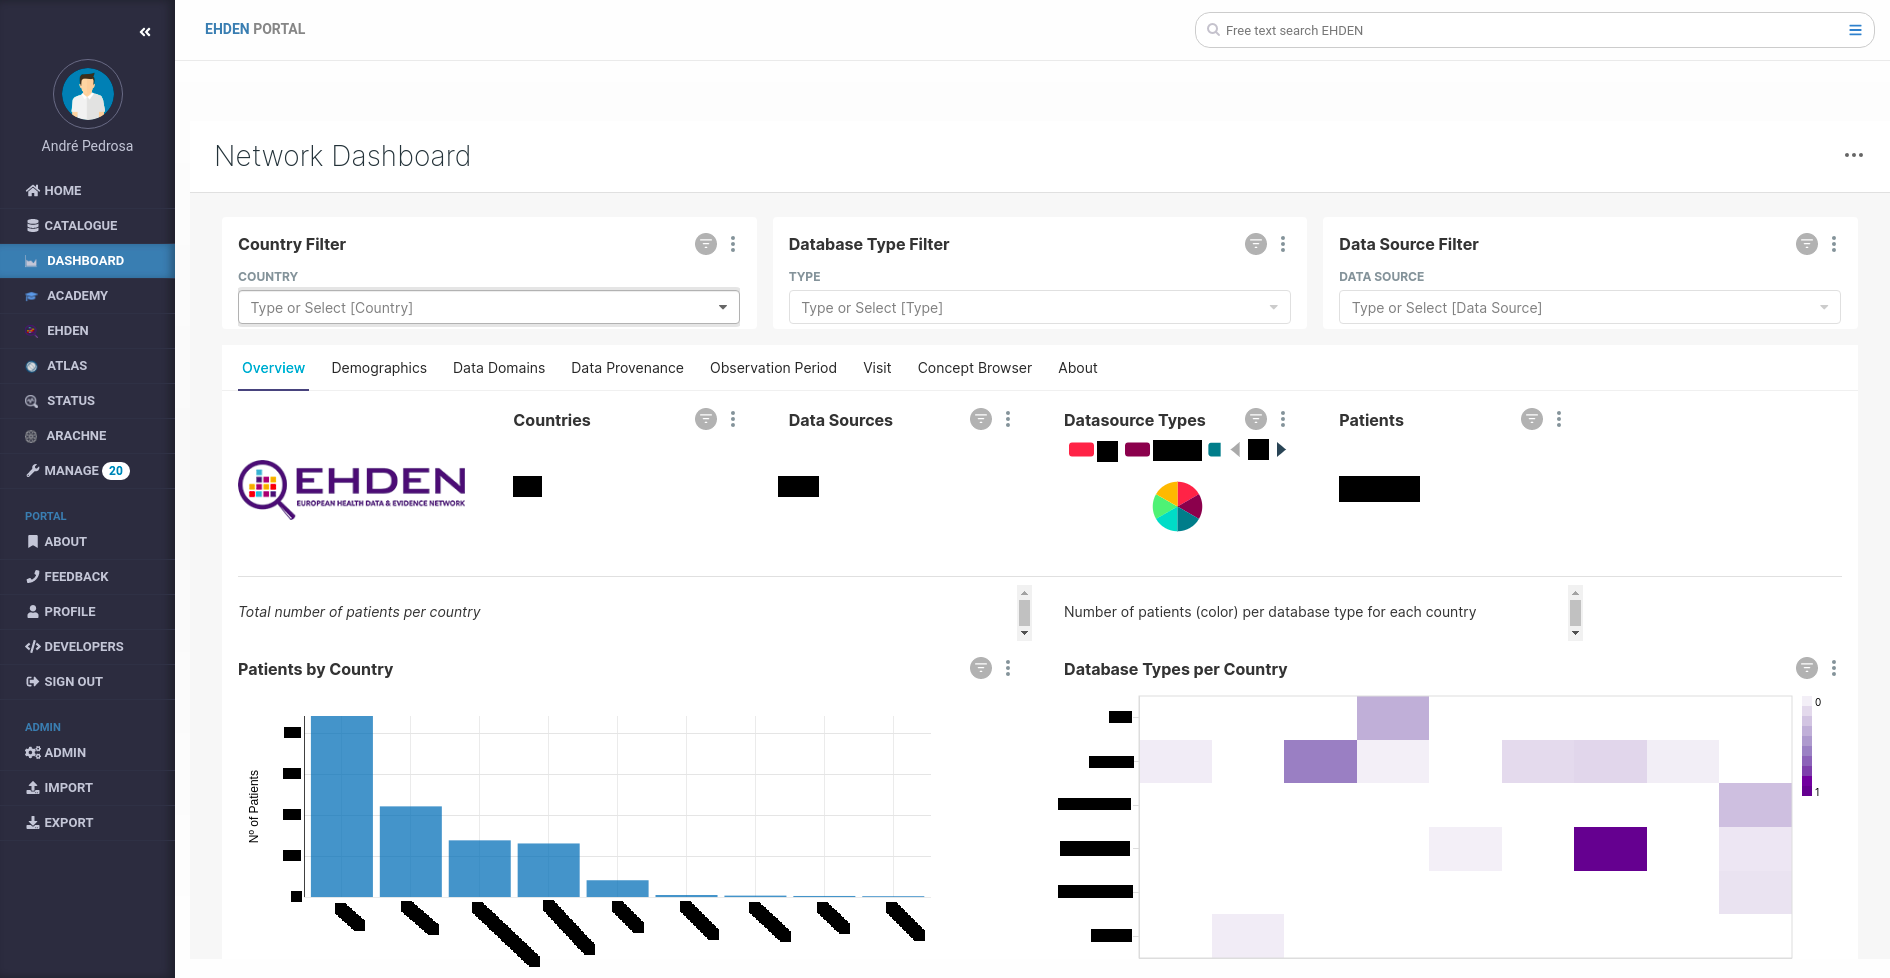
\includegraphics[width=\textwidth]{dashboards}
    \caption{Network Dashboards tool used as a plugin on the \gls{ehden} Portal}
    \label{fig:dashboards}
\end{figure}

\subsection{Publish-subscribe Systems}

During the requirement analysis, one of the non-functional requirements was that ``The system should not require any open ports on the data owners’ deployment environment''.
This implies that the request of communication must be from the agents to the central component, as the contrary can only be achieved if the agent is listening on an open port.
However, data still has to flow from the central component to the agents, such as if the central component wants to know if an agent is active.
One solution would be to have a persistent connection between both ends, however, this could overload the central component if a high number of databases enter the network and it would be continuously taking resources from the data owner's system.

An alternative is to follow a pull philosophy.
The central component can put requests on a message queue, the agent checks periodically this queue and if it finds any request, responds to it.
This can be interpreted as following the publish-subscriber pattern.
This solution also aids achieve the ``Microservice architecture'' non-function requirement as it helps decouple services since they do not require to be aware of each other.
Additionally, the publisher service will not necessarily block waiting for the subscriber service to receive the message, also known as an asynchronous message system.

There are two well know and widely used implementations of such systems: RabbitMQ and Kafka\cite{kafka-vs-rabbitmq}.

\subsubsection{RabbitMQ}

It is recognized implementation of the \gls{amqp} protocol, which this last appears appeared from the need to have interoperability between distinct asynchronous messaging systems.
Before the specification of the \gls{amqp} protocol, there were already several standards for synchronous messaging, however, the asynchronous world did not have such standards.
There was the open \gls{jms}, however, it was limited to java and was simply an interface standard, not specifying a standard protocol.
\gls{amqp} defines a binary protocol implementation, ensuring interoperability between tools implementing the protocol individually.

igure \ref{fig:rabbitmq} presents the architecture of RabbitMQ/\gls{amqp}.
The message brokering responsibility is divided into exchanges and message queues:

\begin{itemize}
    \item Exchange: Accepts messages from the publishers and, based on a set of rules routes, messages to the indicated queues;
    \item Message Queue: Holds messages and sends them to the consumers
\end{itemize}

\begin{figure}[H]
    \center
    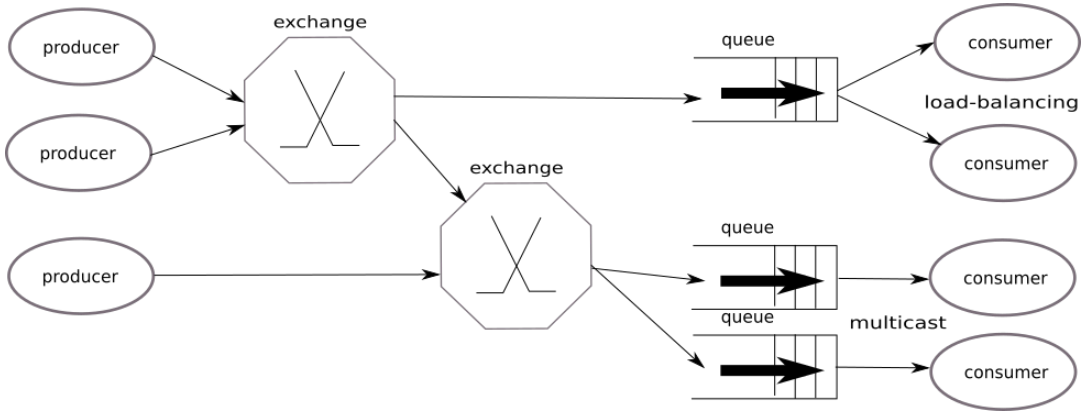
\includegraphics[width=.9\textwidth]{rabbitmq}
    \caption{RabbitMQ(AMQP) Architecture. Retrieved from \cite{kafka-vs-rabbitmq}}
    \label{fig:rabbitmq}
\end{figure}

\subsubsection{Kafka}

Kafka was built at LinkedIn, as its central event pipelining platform.
Before developing it, the team tested alternatives, such as ActiveMQ, a popular messaging system based on \gls{jms}.
However, two problems arose during production tests:
\begin{enumerate}
    \item If the queue started filling up to the point of not being able to store all the messages in memory, performance would sharply drop due to I/O;
    \item To be able to send the same data to a different consumer implies duplicating that data in another queue.
\end{enumerate}

They concluded that the explored messaging systems were designed to target low-latency use cases instead of high-volume scale-out deployment that was needed at LinkedIn.
The team decided to build their custom infrastructure that produces efficient persistence, supports several consumers with a low-performance penalty, and mainly supports distributed consumers while maintaining a real-time messaging abstraction usually obtained from messaging systems.

As a result, the produced system is a scalable publish-subscribe messaging system designed around a distributed commit log.
With this, high throughput is achieved due to data being written to log files with no immediate flush to disk, which allows to build the system with efficient I/O patterns.

The high-level architecture of Kafka is presented in figure \ref{fig:kafka}.
Producers send messages to a Kafka topic.
Each topic is distributed over a cluster of Kafka brokers, with each broker holding zero or more partitions of a topic.
A partition is an ordered append-only log of messages that are persisted in disk.
All topics are accessible for reading by any number of consumers, and new consumers have no performance penalty.
Due to its simple storage layout, every time a producer publishes a message to a topic, the broker simply appends the message to the file corresponding to the associated partition.

\begin{figure}[H]
    \center
    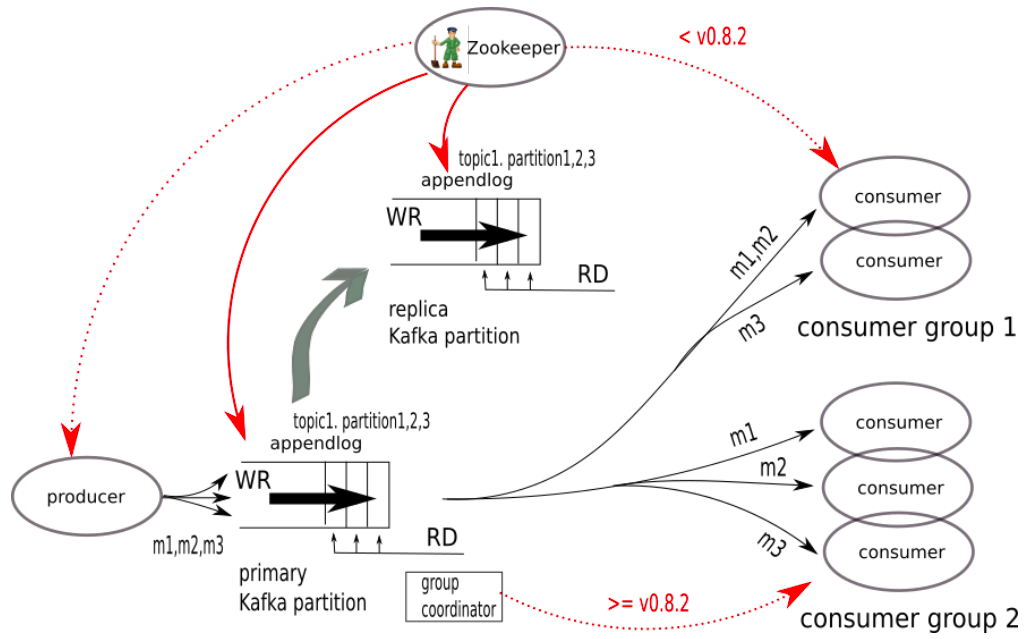
\includegraphics[width=.8\textwidth]{kafka}
    \caption{Kafka Architecture. Retrieved from \cite{kafka-vs-rabbitmq}}
    \label{fig:kafka}
\end{figure}

In contrary to the regular publish-subscriber system, the concept of a consumer in Kafka is generalized to be a group of co-operating processes running as a cluster.
Because of that, a message in a partition of a topic is delivered to only one consumer of a group.
Then, partitions allow to control the level of parallelism of consumers, as different partitions of a topic are assigned to different consumers of a consumer group.

In the end, to achieve the high-throughput requirements, Kafka went on a different road compared to the classic principles of messaging systems in several ways.

\begin{itemize}
    \item It partitions up data so that the production, brokering, and consumption of such can be handled by a cluster of entities that can be scaled as load increases;
    \item Messages are not removed from the log, instead, they can be replayed by consumers;
    \item Reader progress is maintained only by the consumers, so message deletion can only be managed based on a retention policy setting, based either on message count or age;
\end{itemize}

\par\noindent\hfil\rule{.6\textwidth}{0.4pt}\hfil

Originally, the intent was to use a publish-subscriber system just for the communication between the agents and the central component.
However, Kafka has some functionalities that appeal to use also to manage metadata, working as a central component.
Having long-term message storage allows to easily build a fault-tolerant system since consumers can easily replay the message received on a topic.
Furthermore, due to the popularity of Kafka, several libraries and frameworks were developed to extend their usage.
One of them is Kafka Connect, a framework that allows to reliably and easily stream data between Kafka and external systems.
There is also a Kafka Streams\footnote{\url{https://kafka.apache.org/documentation/streams/}} library to perform processing on streams of data on top of Kafka.
As stated before, a different application might not be expecting the entire data from the databases, for that, stream processing features could be useful to filter the data before reaching the target applications.
Finally, with its easily scalable modular architecture, Kafka is well suited to our use case.

\subsection{Kafka Source Connectors}
% kafka tem algumas appllicação ja devenvolvida que tiram dados de uma source e metem mensagem no kafka
% fetch from files or from tables
% falar nas varias opcoes consideradas. as the tables não davam tudo duma vez, e as alternativas de ficheiros não davam feedback de quando tudo ja tinah sido uploaded
% o que eu escolhi da feedback de quando todos os records estão kafka e quantos records foram escritos
% a tabela implica ter esses dados guardados sempre. em differentes runs de achilles (em que os dados têm de ser apagados) eventos falsos de deleção seriam enviados

At this point, we need to find a way to move the data extracted from the database into Kafka.
As mentioned previously, the Kafka Connect framework allows to easily import and export data between Kafka and third-party systems.
Such framework provides plugins called connectors that can be of two types: source, which brings data into Kafka, and sink, which transports data from Kafka into another system.
At this stage the source connectors are more important, however, the sink connectors will still come into use further in the system.

Since the extraction of metadata through the Catalogue Export R package is a bulk process, in other words, a set of metadata metrics are extracted from the database at once, the source connector should handle the data in the same matter.
As there is no way to know, on the central component side, when all the data is in Kafka, the connector should deal with metadata as a bounded source of data, providing some kind of feedback that all data was uploaded to Kafka.

Confluent\footnote{\url{https://www.confluent.io/}}, a streaming platform based on Kafka that aims to aid in optimizing and managing Kafka clusters, has available a search engine, Confluent Hub\footnote{\url{https://www.confluent.io/hub/}}, that allows searching for Kafka connectors and more.
The different connectors available range from known database systems (MongoDB, InfluxDB, ...) to internet protocols (\gls{http}, \gls{ftp}, ...)
In our case, considering that no other application will be running along with the agents, the only storage options available are either a single table on the data owner's relational database or a directory on the disk where metadata is placed in files.

After researching on the Confluent Hub, three connectors were found to suit the possible storage options:

\begin{itemize}
    \item \gls{jdbc} Source connector\footnote{\url{https://www.confluent.io/hub/confluentinc/kafka-connect-jdbc}}

        \begin{list}{}{}
            \item It has four different modes of capturing data from tables.
                Three of them provide incremental information, sending a message to Kafka after a row of a table or a custom query is created or updated.
                The difference between these three modes is from what columns the connector tries to infer that a row has changed.
                These are not suitable for our use case, since it treats a table as an unbounded source of data.

            \item The other mode available is bulk, which sends all the rows of a table in one go.
                However, this process isn't performed based on updates on data, instead, it is executed periodically on a configured interval.
                Furthermore, no feedback is provided after all the data is present in Kafka.
        \end{list}

    \item FileSytem Source connector\footnote{\url{https://github.com/mmolimar/kafka-connect-fs}}

        \begin{list}{}{}
            \item On the contrary to the first connector, this one uses file systems as the source to insert data into Kafka.
                Not only supports fetching files from a local file system, but also widely used cloud storage solutions such as \gls{hdfs}, Google Cloud Storage, and others.
                In our case, we would be using the local file system approach, whereby the data owner places the output files of the Catalogue Export R package on a specified directory.
                As both the extracting tool supports extracting the gathered metadata into a \gls{csv} file and the connector has a specialized reader to parse files in that format, that would be the agreed format to use.
                The connector also supports either moving or deleting files once they are entirely uploaded into Kafka.

            \item As a downside, this connector does not provide any feedback once it finishes uploading the file.
        \end{list}

    \item FilePulse Source connector\footnote{\url{https://github.com/streamthoughts/kafka-connect-file-pulse}}

        \begin{list}{}{}
            \item This connector, is similar to the previous one, as it allows to load data from files into Kafka, having the possibility to also load from other file system solutions.
                It supports reading \gls{csv} files, as it allows having a cleanup policy, which can move or delete files after they are uploaded.

            \item However, contrary to the previous connector, this one sends messages regarding the progress of the upload of the file to a separate topic.
                Not only sends when it ends but also sends the number of rows/messages that were sent into Kafka, which is ideal for our use case, as we can know when the whole file is processed if the rows go through a processing stream on Kafka.
        \end{list}

\end{itemize}

\subsection{Agent Final Architecture}
% docker to facilitae deploymente of agent (will require a little intro to docker)
% data owners should automatize (if they want) the process of achilles extracting data from their databases
% send data to kafka
% responde to health check messages
% automação da extração está nas mão do data owner mas existem ferramentas simples como o crontab que executam commandos a determinadas horas

At this point, we have all the building blocks to set up an agent and make it ready to deploy on the data owners' local system.
The agent will have two internal components:

\begin{itemize}
    \item One will be the FilePulse Source Kafka connector, which will parse the files provided by the data owners and insert their data into Kafka.
        It is important to note that both the metadata and the upload notifications use different topics for each database.
        This was decided because, otherwise, some processing would be required on gathering data of a specific upload from the main topic, that would contain messages from different uploads of different databases.
        The available \gls{csv} reader of this connector allows performing transformations on the data before sending it to Kafka.
        Such transformations include ignoring empty rows, converting values on a row, among others.
        One convenient transformation available transforms the string data of a row into a structure, so data sent in Kafka's messages values is a \gls{json} value instead of a string one.
        This avoids further on the system having to parse strings received from this connector to get a specific field from the data.

    \item The other component is the Health Check Handler.
        It is in charge of sending messages periodically, telling that the agent is active, so when the admin checks the status of the agents it gets a more updated Last Time Active metric.
        As this periodic send of ``I'm active'' messages will not be that regular, one to two times a month, the admin can request an agent to answer if it is active, and it will be this component in charge of sending a response.
        Regarding this last component, as it needs to be developed from scratch, it is a great opportunity to test new technologies that are not so commonly taught on a regular Informatics Engineering course.
        By technologies, we intend to refer to the programming languages used.
        The most popular and used ones are Python and Java, however, other programming languages appeared and are starting to gain terrain on the wap app development.
        Examples of such programming languages are Rust\footnote{\url{https://www.rust-lang.org/}} and Go\footnote{\url{https://golang.org/}}.
        According to the 2020 Stack Overflow Developer Servey~\cite{so-survey}, Rust is the most loved language among developers, and Go, in terms of most popular languages, just stands behind equivalent languages such as Python, Java and C Sharp.
        Besides behind the most loved language, Rust's ownership model, which increases memory safety with compile-time checks, is something that is not present in other languages, and newcomers will have a not-so-appealing learning curve.
        For that, the decided language to use was Go, which will also be considered for other components of the system that eventually require to be built from scratch.
        The popularity of Go mainly comes from its simplicity, as it has a C-like syntax, and for having concurrency mechanisms builtin in the language, not requiring an external library to implement such concepts.
\end{itemize}

Now the only missing part of the agent is how to deploy it.
As said in the requirement analysis, the deployment of the agent should be an easy process.
At its core, the FilePulse connector is a Java application.
With that, the agent requires that the data owner has both Go and Java runtime dependencies available so that the agent could be deployed in their local system.
This could cause problems for the data owners since he could already have these dependencies, but the wrong versions, and installing a new version could cause problems.
Also, different data owners could use a different operating system, which could change the way dependencies have to be installed, so it's hard to create install instruction that covers all the possible deployment environments.
With the emerge of cloud computing, virtualization solutions started to be used, allowing to use a single physical machine for several purposes, taking more advantage of the available hardware.
To achieve this, a software called Hypervisor sits on top of the host machine, which divides the hardware resources so that they can be used by separate virtual machines~\cite{virtualization}.
However, such virtualization technology emulates an entire operating system, on every virtual machine, which is a heavy option to deploy a simple agent.
A more convenient virtualization technology is containerization.
Such technology can be seen as a very lightweight virtual machine since a container is a package of software code with just the application to run and the necessary dependencies.
Containers are also more efficient in taking advantage of the hardware available, as portions of the hardware are not statically allocated to each container~\cite{containers}.
Containers run in an operating system as they were yet another process, but for the code running in a container, the appearance is that they are running in an isolated machine.

\begin{figure}[H]
    \center
    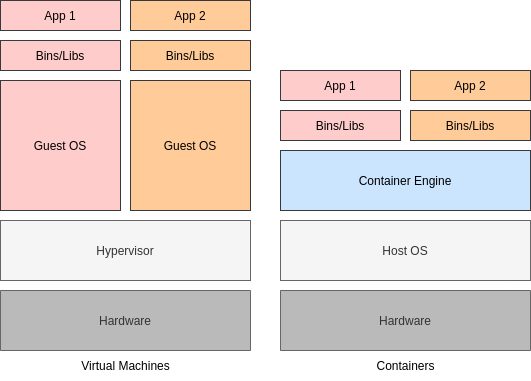
\includegraphics[width=.6\textwidth]{virtualization}
    \caption{Comparison between virtual machines and containers}
    \label{fig:virtualization}
\end{figure}

Figure \ref{fig:virtualization} presents a visual comparison between virtual machines and containers.
As can be seen, the virtual machine technology has to simulate two operating systems, in contrast to the container solution where there is only one operating system and the container engine.

With a deployment strategy in mind, figure \ref{fig:agent-architecture} shows the final architecture around the agents and pieces that connect to the data owner's system.

\begin{figure}[H]
    \center
    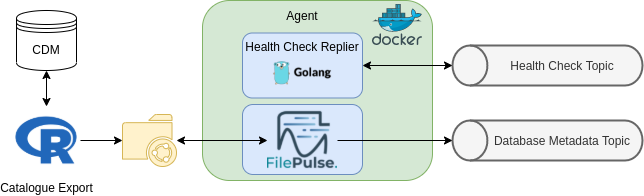
\includegraphics[width=\textwidth]{agent-architecture}
    \caption{Agent + Catalogue Extractor architecture}
    \label{fig:agent-architecture}
\end{figure}

Docker\footnote{\url{https://www.docker.com/}} is an industry standard that facilitates the process of creating, managing and sharing containers.
Developers can share their built containers, called Docker Images, in Docker Hub\footnote{\url{https://hub.docker.com/}}, which then can be used to build more specialized containers.
For example, there are official Docker images available with Python pre-installed. These images can be used by developers that want to deploy their Python apps with Docker, not having to bother installing a specific Python version.

With that, the agent will be distributed to the data owners as a Docker image.
However, data owners have to perform two tasks before starting the agent.
One is to choose which directory will be shared with the agent's container.
This can be achieved with the Docker's volume system, where a directory on the host operating system will be bound to another within the container.
The second step is to define a set of environment variables that will be unique to this agent:

\begin{itemize}
    \item AGENT\_DELETE\_CLEANUP\_POLICY: defines whether or not files must be deleted after their data is uploaded into Kafka.
        By default, the file is moved into a \textit{succed} directory, so this variable is optional.
    \item AGENT\_DATABASE\_IDENTIFIER: an identifier provided by the admin once the database is registered in the system.
\end{itemize}

After getting the Docker image of the agent, the data owners only have to execute a simple run command where defines the previous decisions:

\begin{verbatim}
docker run
  -v ./catalogue_export_files:/app/catalogue_export_files
  -e AGENT_DATABASE_IDENTIFIER=unique_db_identifier
  -d
  AGENT_IMAGE
\end{verbatim}

Next is the description of each option:
\begin{itemize}
    \item -v: binds a host directory to the one inside the container where FilePulse will read files from;
    \item -e: sets the AGENT\_DATABASE\_IDENTIFIER environment variable
    \item -d: runs the container in daemon mode
\end{itemize}

Regarding the extraction tool, we will also distribute a Docker image with the necessary dependencies preinstalled, where data owners will have to provide the necessary information for this tool to access the \gls{cdm} database and define a volume so files containing the metadata are accessible to the agent.
Concerning the automation of the extraction process, the image will contain Linux's cron command-line utility, which allows to schedule tasks.
The data owners will only have to provide the periodicity of the extraction process, using Cron's time and date syntax to define a cronjob.
\begin{verbatim}
.---------- minute
| .-------- hour
| | .------ day of month
| | | .---- month
| | | | .-- day of week
| | | | |
* * * * *
\end{verbatim}
If the extraction process were to run two times a month at three in the morning, the following configuration is used:
\begin{verbatim}
0 1 1,15 * *
\end{verbatim}
The task will execute on days 1 and 15 of every month at three in the morning.
However, if it is preferable for the data owner, he can set up his automation, or no automation, of the extraction process.

\section{Publishing}
% data is in kafka. what do we have to do to reach the applications
% idealmente usamos o kafka e afins para tudo, não tendo de desenvolver nada
% need to send custom data on a CUSTOM FORMAT to a custom REST endpoint
% Kafka Sink Connectors (The target REST API is not customizable, such as the data format ) - need for a sender application
%  https://www.confluent.io/hub/confluentinc/kafka-connect-http
%  https://docs.confluent.io/kafka-connect-http/current/overview.html
%   - envia um pedido para cada row dos dados do ficheiro
%   -  que tal dar aggregate tudo numa mensagem? resolve? não é aconselhavel ter mensagens grandes
%   - não deixa customizar body se eu quiser fazer algo {data:{patients_num:1, ...}}
% No known end on kafka topics/streams - require some management on top of kafka

At the moment, we can deploy several agents on the data owners' local systems and have a set of Kafka topics to where data is uploaded when \gls{csv} metadata files are generated.
We now need to send this data to the web application in form of \gls{http} requests.
Ideally, no other component is required, and Kafka is enough to act as a central component of our metadata publishing system.
With that, a search must be performed to find Kafka sink connectors, which should do the inverse of what the FilePulse connector does on the agent side, which is getting data from Kafka into an external system, in this case in form of \gls{http} requests.

Resorting to Confluent Hub again to search for sink connectors, only one allowed sending Kafka data in \gls{http} requests: HTTP Sink Connector\footnote{\url{https://www.confluent.io/hub/confluentinc/kafka-connect-http}}.
However, it does not meet some of the requirements.
Since different applications expect the data in distinct formats, requests need to be customizable, however, the connector does not allow to customize the request.
The data sent, will be the same as the one present on the value of the Kafka message and the connector only allows to send requests with the \gls{http}'s POST or PUT methods.

Furthermore, by default, this \gls{http} connector will send a request for each Kafka message.
The connector being used on the agent sends a message for each row of the catalogue export \gls{csv} file, which would mean that this \gls{http} connector would send several \gls{http} to an application related to the same upload.
The \gls{http} connector supports batching messages together, on the same request, however, messages are stored in memory until the batch size is not reached, which could cause memory problems if the upload contains a high number of metadata metrics and also if several databases upload at the same time.
Additionally, the number of messages sent by a database is dynamic, which the \gls{http} connector does not support, since it gathers a finite number of messages.
This problem will always exist due to the nature of Kafka, where topics can be treated as streams of data, which do not have determined start and end, and there is always data flowing.

\section{Metadata Manager}
% centralized entity working on top of kafka, dealing with the unbounded format of data in Kafka
% performs operations on top of kafka
% transforms the data to the required format
% sends to the specific application's endpoint
% 5 components

To takle the problems mentined previously, new components need to be developed.
Such group of components will be called Metadata Manager, which will perform operations on top of Kakfa.
The main issues that will be addressed are allowing to customize the requests that are sent to the applications and dealing with the unbounded factor of Kafka topics/streams.

Figure \ref{fig:metadata-manager} presents an overall architecture of how internal components of this Metadata Manager will be organized.
For the communication between components, Kafka topics are used, however their organization will be detailed when going over the several components next.

\begin{figure}[H]
    \center
    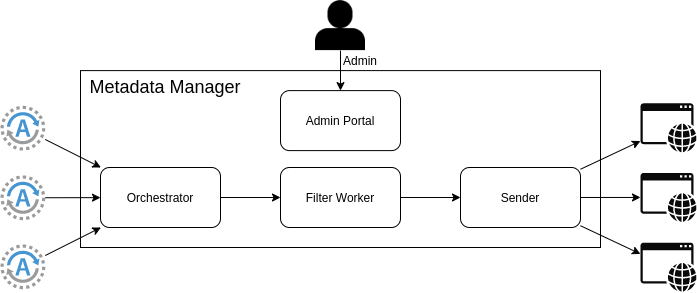
\includegraphics[width=\textwidth]{metadata-manager}
    \caption{High-level architecture of the Metadata Manager components}
    \label{fig:metadata-manager}
\end{figure}

As these components will be implemented from scratch, the programming language that will be used is Go, if applicable, for the same reason explained in the Health Check Handler component of the agent, try new emerging technologies beyond the most popular ones.

\subsection{Filter Worker}
% lets do it in go cause lets explore
% ksql introduced. easily filter data with select \_ where \_
% select and filter the data comming from the databses
% only process data of a single database at a time. handling multiple is the same is hard to handle and hard to scale
% scalable: several pipeline worker applications

Data comes from the agents in several Kafka messages, which need to be gathered together to then be used to build the custom request for each application.
As gathering all the uploaded data in memory is not a scalable option, and implementing a system with memory usage management is a complex task, the system must first filter out unnecessary data and only allow the Admin to build and send the request to the applications.
A Filter operation will remove entire rows, however, only a subset of columns might be required, for that, the system should also allow choosing which columns of the metadata are required.

That's what the Pipeline Worker component is supposed to do.
Extract only the essential data from all the data uploaded by an agent and then send it to the Sender component, who will be in charge of building and sending the request to the applications.

Since data is already in Kafka, we can take advantage of its stream processing features to filter data received from the agents.
But, once again, streams imply an unbounded size of data, so additional processing has to be built on top of such stream processing.
If a stream is created to get the data that satisfies a given condition, we need to make sure that all the uploaded data went through that given stream.
This can be achieved by creating two streams with opposite filtering conditions (figure \ref{fig:filter-workers}).
\begin{figure}[H]
    \center
    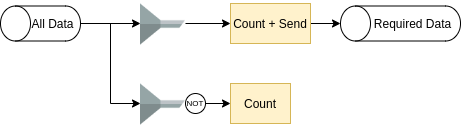
\includegraphics[width=.7\textwidth]{filter}
    \caption{How Filter Workers process unbounded data received from agents}
    \label{fig:filter}
\end{figure}
One will be used to get the actual data, the other, with the filtering condition negated, will be used just as an auxiliary.
At the end of each stream, a component will count the number of records that went through.
When both sum up to the number of messages sent by the agent, we can know for sure that all data was filtered and the Sender component can use the result data.
As the stream with the negated filtering condition will be used to just get a counter, there is no need to send the actual data on that stream, for that a single byte is sent to avoid wasting memory resources.

To develop these filtering streams, there are two options:
\begin{itemize}
    \item Kafka Streams: A Java library to process and analyze data that is already present on Kafka.
        Using it would imply implementing this Filter Worker component in Java, however, from the explanation of how a filter will be implemented, there will be several threads involved, requiring communication between them.
        Developing such an environment in Go is much easier as concurrency mechanisms are built in the language itself, and also if the number of filters gets high, threads might start to slow and use a lot of memory, as each has its own address space.
        Go, on the other hand, has goroutines, lightweight threads managed by the Go runtime, which run in the same address space.
        Using Kafka Streams would also imply that the conditions defined by the Admin, would require to be written in Java code.
    \item KsqlDB~\cite{ksql}: is a database that allows assembling stream processing applications on top of Kafka.
        It combines the power of stream processing with the known feel of a relational database through a \gls{sql}-like syntax, so stream applications can be set up with just \gls{sql} statements.
        As the data sent by the agents are messages extracted from a \gls{csv} file, the data can also be interpreted as a table, so the \gls{sql} language feats well in this case.
        It provides a \gls{rest} \gls{api} interface, so using KsqlDB does not bound the implementation to a specific language.
\end{itemize}

We opted to go with KsqlDB as it allows us to build the application in Go, taking advantage of its lightweight goroutines, allowing the system to scale better and the system to receive data from more databases.

Until now, it was assumed that each application has its filtering condition over the data.
However, two distinct applications might benefit from the same filtering condition, for that, the relationship between filters on data for an application is a one-to-many relationship, so the data resulting from one filter might be used to build and send data to several applications.

In terms of internal organization, displayed in figure \ref{fig:filter-workers}, the main goroutine is in charge of managing the several active Filters, stopping existing ones and starting new ones, according to the orders received from the Admin Portal component.
Each filter runs in a separate goroutine, which by itself launches other two goroutines.
One is in charge of counting the data that comply with the filtering condition and the other is counting the number of messages that do not fit the filter condition.
The count of messages filtered is monitored by the main goroutine of each filter.
When it reaches the number of messages that the agent sent, it tells the other child goroutines that they can stop reading from the streams, and sends a notification to the Sender component telling that data is ready to be sent.

\begin{figure}[H]
    \center
    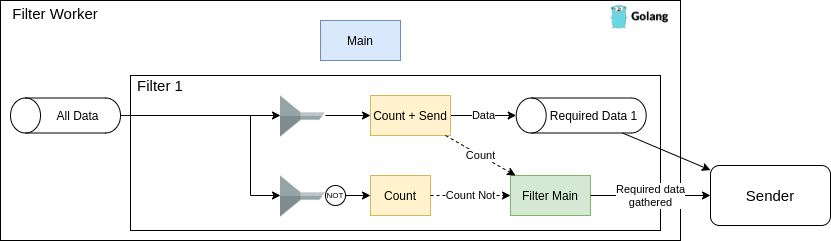
\includegraphics[width=\textwidth]{filter-workers}
    \caption{The internal organization of a Filter Worker}
    \label{fig:filter-workers}
\end{figure}

Note that the ``All Data'' topic is unique to the Filter Worker application, this means that on a Filter Worker application there can be several Filters running at the same time.
Also, this means that a Filter Worker application will obtain the data to all the filter conditions that were defined, at the same time, for one single database.
The system then allows scaling, by running several Filter Worker applications at the same time, with that, several Filters can be run for different databases at the same time.

\subsection{Orchestrator}
% why do we need this. why do not the workers read directly from the database.
%  Cause wokers use ksql, and it does not allow to create a stream and start reading at a giving time. either start or end.
% To ensure multiple records of multiple databases are not processes at the same time, this component redirects the data from databases to the pipelines workers preventing the previous problem
% why not use ksql? cant set offset to read from. either always read from start or always read from end
% why java? (only it contains a kstream api) and we use it to redirect messages from one topic to another
% 2 threads: one reads uploads and creates streams of data, another closes streams once all data was transfered

As multiple Filter Worker components might be running at the same time, there needs to be a way to redistribute the load among the running instances.
Since agents publish a topic when the upload process is done, a goroutine on each Filter Worker could dynamically create the required processing streams on the data topics of the databases that performed the upload.
However, as all data on the data topic of a database might not be related to the same upload, due to the retention policy chosen, we require to start the transmission of messages at a given offset of the data topic.
Such a thing is now achievable with KsqlDB since it only allows to read either from the latest or earliest record.
As an alternative, Kafka Streams allows achieving this.
This will require that this redistribution of work has to be written in Java, but as an advantage removes, this responsibility of reading data from databases' topics from the Filter Workers components, allowing for more concrete and small components.

Previously, it was mentioned that the concept of a consumer in Kafka is a group of co-operating processes running as a cluster, so messages of a topic are distributed in a balancing manner, sending a message to only one process of a given group.
For that, there is no need to implement a balancing algorithm to balance the data uploaded from the agents, as Kafka can achieve that already.

\begin{figure}[H]
    \center
    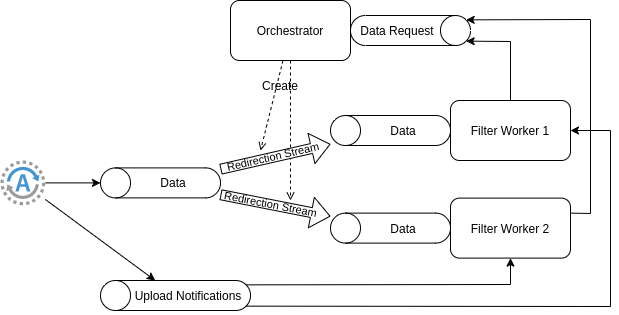
\includegraphics[width=\textwidth]{orchestrator-role}
    \caption{The workflow of how data uploaded from the agents is balanced across Filter Workers instances}
    \label{fig:orchestrator-role}
\end{figure}

As shown in figure \ref{fig:orchestrator-role}, every Filter Worker will have a consumer for the Upload Notifications topic, which all will belong to the same group.
This ensures that only one Filter Worker instance will receive a given message, thus implementing a balancing policy with Kafka.
On the Filter Worker component, another goroutine will have to be created, which will consume from the Upload Notifications topic and then broadcast this notification to the active Filters (Figure \ref{fig:filter-worker-uploads}).
\begin{figure}[H]
    \center
    \includegraphics[width=.6\textwidth]{filter-worker-uploads}
    \caption{New ententies achitecture on a Filter Worker component}
    \label{fig:filter-worker-uploads}
\end{figure}
This new entity, Upload Watcher, will broadcast the notification using Go's channels, a built-in language feature that allows having pipes of communication between goroutines.
Additionally, this entity will also send a message to the Data Request topic, telling the Orchestrator that his Filter Worker instance is in charge of parsing the data associated with a specific upload of an agent.
The Orchestrator will then create the necessary redirection stream between the database's data topic and the specific Filter Worker instance's data topic.

Following the same balancing concept used for the Filter Workers, the same can be applied to the case of scaling the number of Orchestrators.
Different Orchestrator instances will consume from the Data Request topic belonging to the same group, balancing the work of redirecting upload data over several Orchestrator instances.

Internally, the Orchestrator is composed of two entities:
\begin{itemize}
    \item one that consumes from the Data Request topic and creates the redirection streams from databases' data topics into the Filter Workers' data topics;
    \item for each message received by the previous entity, another entity checks when all data reached the data topic of the target Filter Worker instance and closes the stream once that happens.
\end{itemize}

\subsection{Sender}
% sends/publishes the data resulting from the pipelines, to the application's endpoints
% why python? cause jinja and pandas (people know how to use)
% since data was filtered, small data is in memory now

At this point, the system contains the data required to build the requests and then send them to the applications.
It is now required to get, from the Admin, the configuration of the \gls{http} request to send the data.
An interface to build \gls{http} requests would require several components to allow customizations of the several items of an \gls{http} request: authorization, headers, method, \ldots
To allow flexibility on the configuration of the \gls{http} request, such an interface would either be too complex or some features would not be allowed to simplify the implementation of such interface.

Many programming languages have libraries that allow performing \gls{http} requests and customization is provided by passing different parameters to functions of such libraries.
Such parameters will then go over a validation process, avoiding the use of invalid values, such as sending a request with REPLACE as the \gls{http} method for example.
With that, it would be easier to make use of such libraries, and then Admins would provide the arguments for a function that performs \gls{http} requests.
The system would provide the data that resulted from a filter to the Admin, and then he would build a structure where they specify the required and additional optional parameters of an \gls{http} requests library's function.

On top of that, the request for each database within the same application might be different, one might use the URL ``http://app.com/data/db1/'' and another use ``http://app.com/data/db2/'', for that the system must provide additional data besides the data filtered, such as the database information.

Basically what the Admin needs to provide the system is a template defining the parameters to a function of an \gls{http} request library function.
On this template, the Admin can use placeholders to define where the system should insert certain data.
Django contains a template system that allows building dynamic \gls{html} pages.
The developer can write a normal \gls{html} page and then, using a special syntax, can tell where Django should insert data to fill the page.

\begin{verbatim}
<html>
  <head>
    <title>{{ app_name }}</title>
  </head>
  <body>
    <h1></h1>
  </body>
</html>
\end{verbatim}
In the example above, \{\{ \textit{app\_name} \}\} will be replaced by the value of the variable app\_name.

However, the entire Django framework is not required to build the Sender component, as the component does not require to either render pages or manage database models.
Only the templating system is required.
Fortunately, there's a Python package called Jinja\footnote{\url{https://palletsprojects.com/p/jinja/}}, which was built based on Django's template system.
It has a similar syntax to the Django Template System providing some additional features and being more pythonic.

For now, let us assume that the template will be an argument defined in each line, it would look something like this:
\begin{verbatim}
method: POST
url: http://www.app.com/data/{{ database_identifier }}/
data: {"patients_number": {{ filtered_data.get("patients_number") }}}
\end{verbatim}
On Jinja, placeholders are defined within \{\{\ldots\}\} tags, so it would look for the database\_identifier variable and execute the get method of the filtered\_data variable.

While building its template, the Admin must have access to the filtered data, which, on the example above, was exposed through a filtered\_data variable.
As data is in a Kafka topic, the system must provide an abstraction to easily access such data.
Once again, since data is extracted into a \gls{csv}, it can be interpreted as a tabular type data.
Two programming languages suited to read and manipulate data in this format are Python and R, which are widely used on data analysis applications.
R is a more specialized language than Python since is suited for statistical analysis~\cite{r-lang}, however, Python is more popular, as there are many data analysis and machine learning packages written in it.
As the Admin will mainly just want to access the data, the chosen approach was to expose the data using the Pandas Python package\footnote{\url{https://pandas.pydata.org/}}.
It contains a DataFrame data structure, which is widely used in data manipulation and analysis applications written in Python.

With Jinja and Pandas, the Admin can customize the request that sends the data to the applications, however, there is a use case that there is no possibility to achieve with this implementation.
It was mentioned previously that the \gls{ehden} project uses a separate tool as a plugin of the \gls{ehden} Portal to build visualizations allowing for better comparison between databases, which is named Network Dashboards.
Data is inserted into the tool by uploading a file into a form, which is not possible to reproduce with the current implementation.
In Python, the most popular library to perform \gls{http} requests is called requests\footnote{\url{https://docs.python-requests.org/en/latest/}}.
It contains several specific functions that allow performing any type of request.
Files can be sent with this library by passing a file pointer as one of the arguments.
In Python, a file pointer can be acquired by opening a file on disk.
With this, the system has to provide a way to allow the Admin to insert this file pointer in its template of the \gls{http} request.

To avoid having to create a parser to read a custom structure of key-value pairs where Admins define the parameters of the request, it would be ideal that the template could be generated directly into a Python data structure.
This can be achieved by running code dynamically.
When the template provided is rendered, replacing the placeholders by their values, a string value is generated.
We can then treat that string as Python code and execute it.
The system will require that this code returns Python's key-value data structure called dictionary, which can then be used to pass arguments to the requests function that performs the \gls{http} request since Python allows to provide arguments to a function with a dictionary.

Let's sum up the process of building and sending the requests to the applications (Figure \ref{fig:sender-request}):
\begin{enumerate}
    \item The Admin defines a template with placeholders;
    \item Once data is received by the Sender component, the template is rendered and a string will be generated;
    \item The generated string will be executed as a Python code returning a Python's dictionary;
    \item The dictionary is used to provide the parameters to the request function to perform the \gls{http} request.
\end{enumerate}

\begin{figure}[H]
    \center
    \includegraphics[width=\textwidth]{sender-request}
    \caption{Process of generating the parameters of the \gls{http} request to send to an application}
    \label{fig:sender-request}
\end{figure}

Note that, in figure \ref{fig:sender-request}, the value of the files dictionary is a variable name, which will be a local Python variable containing the file pointer to a temporary file containing the records received from the Filter Worker component.

\begin{figure}[H]
    \center
    \includegraphics[width=.5\textwidth]{sender-interaction}
    \caption{Interaction between the Filter Worker and Sender components}
    \label{fig:sender-interaction}
\end{figure}

Regarding how data is transferred from the Filter Worker component to the Sender, figure \ref{fig:sender-interaction} shows a representation of the process.
Once all data was filtered, the main goroutine of each Filter will send a message to the Data Ready to Send topic with the following metadata:
\begin{itemize}
    \item Filter Worker application id: since several could be running at the same time;
    \item Filter id: through what filter did the data go;
    \item Kafka topic offset: wherein Filter's data topic does the data start.
    \item Records count: number of records that meet the filtering criteria;
    \item Database identifier: to what database does the data belong;
\end{itemize}

The internal structure of the Sender component is similar to the Orchestrator components, having the main thread consuming from the Data Ready to Send topic, and then other threads will deal with the work of building and sending the request to the applications.

Scalability is also allowed on this component as multiple Sender components can be running at the same time.
For that, consumers used by their main thread all must belong to the same group to ensure that a message is sent to only one Sender application.

\subsection{Admin Portal}
% search for tecnologies (first: golang pls . https://github.com/qor/admin)
% react or angualr allow more customizability. dont want from scratch. react-admin library
% 2 components: api backend (django) + react frontend
% manage the whole thing. talks to the other components using kafka management topics
% models and their relasionships
% Allows to perform all the use cases

Moving to the component where the Admin will use to manage the whole metadata manager.
It will allow performing the several use cases defined on the requirement analysis stage: managing communities, databases, filters and target applications, and checking statistics of the system.

As this component is mainly just a web interface, a search was performed for Go packages that allowed to create some kind of admin dashboard.
Some solutions were found such as Qor Admin\footnote{\url{https://github.com/qor/admin}} and GoAdminGroup/go-admin\footnote{\url{https://www.go-admin.com/}}.
The first solution had good documentation and features.
It creates management pages for each data model defined, allowing a user to perform the regular \gls{crud} operations on such data models.
However, there was small flexibility on what to display on a display page of a data model.
For example, if a model had an id and a name, only those fields would appear on the display page of such a model.
The second solution had better flexibility compared to the first one, however, page customization was done through a series of function calls which lead to big chunks of code to define a page, consequently, contributing to the maintainability of this component to be hard.

With this, we decided to separate this component into two parts, a web interface app and a backend app exposing an \gls{api} for the web interface app to use.
This allows using technologies that are better suited for such types of applications.
Regarding the web interface, there are several popular web frameworks/libraries such as React\footnote{\url{https://reactjs.org/}}, Angular\footnote{\url{https://angular.io/}} and Vue\footnote{\url{https://vuejs.org/}} that intend to facilitate the process of creating web applications.
However, we didn't want to build something from scratch, for that, we performed a new search for framework/libraries that used those web technologies, but were specialized to build an admin interface.
The solution found was React-Admin\footnote{\url{https://marmelab.com/react-admin/}}, a frontend framework to build data-driven applications.
React~\cite{react} is a library that allows dividing a page into components that can be reused across the web application.
Each component them as an internal state, and React will automatically update and render the associated components as the data changes.
With React-admin, customizations are easily implemented by just creating new components and then adding them to their appropriate place.
Also, such new components are implemented in a combination of \gls{html}, \gls{css} and Javascript, languages that are mainly used to build web interfaces.

Regarding the backend, the React-admin framework already takes care of the communication between the frontend app and the backend app, however, only a set of technologies are supported to use in the backend.
One of the available technologies to use is Django, which must be used alongside the framework called Django REST framework\footnote{\url{https://www.django-rest-framework.org/}}, which allows exposing Django's models through an interface.
Django was chosen over other technologies such as Springboot\footnote{\url{https://spring.io/projects/spring-boot}} or GraphQL\footnote{\url{https://graphql.org/}} due to it managing the models by itself, creating migration files every time data models definition are changed on the Django app, allowing to keep both the business logic and the stored data models in a relational database in sync automatically.
The database used here in conjuntion with Django will be PostgreSQL\footnote{\url{https://www.postgresql.org/}} since it is one of the most popular open-source and free \gls{rdbms}.

With this integration between the frontend app and the backend app set up by React-admin, when defining a page on the front end app, it is only necessary to define to which model is referred to, and then enumerate the wanted fields that must be displayed on the page.
There is no need to implement calls to the \gls{api} exposed by the backend app, as the React-admin framework will take of this automatically.
Additionally, this framework supports relationships, which allows displaying extra data associated with a model, for example, if a database belongs to a community we can also display the Community information on the database page.

\begin{figure}[H]
    \center
    \includegraphics[width=\textwidth]{data-models}
    \caption{Data models managed on the Admin Portal component}
    \label{fig:data-models}
\end{figure}

Concerning the models' organization, figure \ref{fig:data-models} shows the relationship between models of the Metadata Manager system.
Models marks with green the admin can perform all \gls{crud} operations, models in yellow are only for reading as they are created by the Statistics Recorder component, and models in blue are dependent models, which are defined when the main model is created, in this case, FilterSelection entries are created when the Admin is creating a Filter.

\subsection{Statistics Recorder}
% kafka jdbc connector?
% Listens to the kafka topics that are used along the system and transforms into persistent statistics data (sql)
% removes this responsability from the other microservices
% belongs to a separete consumer group

Finally, this last component is in charge of reading messages that are sent between the components described before and persisting some of those messages as statistics of the system, so the admin can consult them on the Admin Portal.
This could also be done on the components that send those messages, however, this way, such components are simpler and have well-defined objectives.

To avoid interfering with the data flow of other components, this Statistics Recorder component should consume messages from the necessary topics using a different consumer group, this way Kafka will send a message of a topic to both this component and the other components.

However, there is no need to develop a component from scratch to perform this.
As we intend to move messages from Kafka into a relational database, we can make use of a Kafka Sink connector.
A connector that allows achieving this is the JDBC Sink connector\footnote{\url{https://www.confluent.io/hub/confluentinc/kafka-connect-jdbc/}}.
We are only required to set up Kafka Connect and launch a task using the JDBC Sink connector for each topic where the messages have to be persisted on the database.

\section{Summary}
% referencias para um anexo onde tem um diagrama completo do sistema
% sistema capaz de automatizar o processo de atualizar metadtados nas apps

This chapter it was explained the entire development process around a system capable of automating the procedure of updating metadata stored on web applications about clinical databases.
A solution was provided to the data owners to automatize the process of extracting metadata from their databases and then the system will make sure that that data will reach the desired web applications.
A complete diagram of the system is present in Appendix \ref{appendix:a}.

%The next chapter will present the system developed in this chapter in action, using an installation of the Montra framework improved in chapter \ref{chapter:metadata-visualization} as a target web application of the metadata.

%\chapter{Evaluation}
\label{chapter:evalution}

\begin{itemize}
    \item target applications, montra + dashboards
    \item step by step
    \item idialmente screenshots
\end{itemize}

\section{Deploymente}
não há necessidade em falar no kafka regestry. no diagrama de deployment, se o fizermos, simplesmente representamos o kafka como um unico container.
eventualmente podemos dividir em kafka broker + kafka zookeper

\section{Network Data Flow}
\begin{itemize}
    \item step by step
\end{itemize}

%\chapter{Conclusion}
\label{chapter:conclusion}

future work:
\begin{itemize}
    \item criar um mecanismo de chaves por communidade. quando uma bases de dados envia dados sabemos imediatamente a que communidade pertence
    \item usar a autenticação do kafka para validar os dados recebidos das bases de dados
    \item criar um mecanismo de teste para as pipelines e subscrições
    \item por enquant a comunicaçãoo no sentido (componente central -> agent) apenas é usada para saber se o agent está ativo. no futuro pode ser usado para outro tipo de comunicacao
\end{itemize}

novas tecnologies (yey). são nices e foram faceis de usar

hopefully is used or gives ideas for future prodution systems

já existe um Pr para o repositorio do montra-pvt, estamos apenas à espera que seja revisto e merged com o principal


% End of Thesis text ---------------------------------------------------------
% Including files is advised:


%Appendix

\backmatter


%Print all used references

\begingroup
\renewcommand{\bibfont}{\footnotesize}

%Redefine References name
\defbibheading{bibliography}[References]{
	\chapter{#1}
}
\SingleSpacing
\setlength\bibitemsep{8pt}
\printbibliography[heading=bibliography]
\endgroup


%Load appendix
%\include{appendix-a}



\end{document}
